\chapter{基于双波长探测的气体浓度检测系统设计}

\section{气体浓度检测原理}

\subsection{Beer-Lambert定律}
Beer-Lambert定律是气体吸收领域最基本的定律,该定律描述的是一束单色平行光经过某种均匀混合的气体吸收后,其透射光强与入射光强之间的关系,即
\begin{equation}
\label{beer_lambert}
I_{t}(\upsilon) = I_{o}(\upsilon)exp(-\sigma_{ext}NL)
\end{equation}
其中,$I_{t}$为透射光强,$I_{o}$为入射光强,$\sigma_{ext}$为消光截面($cm^{2}$),$N$为气体浓度($molecule/cm^3$),$L$为有效光程($cm$)。需要注意的是,公式中的消光截面、入射光强和出射光强都是频率相关的。公式中的消光截面可以分为两部分,即
\begin{equation}
\label{extinction}
\sigma_{ext} = \sigma_{abs} + \sigma_{sca}
\end{equation}
其中,$\sigma_{abs}$为吸收截面,$\sigma_{sca}$为散射截面。在气体检测领域,检测的气体通常为纯气体混合物,气体中很少存在气溶胶或者颗粒物的散射干扰,因而一般忽略散射截面的影响。而当检测对象为气溶胶时,吸收截面相对于散射截面会小很多,则会忽略吸收截面。针对气体检测,我们可以得有
\begin{equation}
\label{absorption}
I_{t}(\upsilon) = I_{o}(\upsilon)exp(-\sigma_{abs}NL) = I_{o}(\upsilon)exp(-S(T)\phi(\upsilon)NL)
\end{equation}

对公式\ref{absorption}做简单变形之后我们就可以得到气体的透过率(Transmittance Function)和吸收率(Absorption Function):
\begin{equation}
\label{transmittance_fuction}
TR = I_t(\upsilon)/I_o(\upsilon)
\end{equation}
\begin{equation}
\label{absorption_fuction}
AF = 1 - TR
\end{equation}

\subsection{非色散红外吸收光谱学}
非色散红外吸收光谱学(Non-dispersion infrared absorption spectroscopy, NDIR)通常通过检测两个不同波长的激光经过气体的吸收,一个激光波长$\lambda_{on}$位于气体的吸收峰上得到$I_{on}$,另一个激光波长$\lambda_{off}$位于该吸收峰边上得到$I_{off}$,根据气体的吸收截面与有效光程,从而推算出气体的浓度信息,测试装置如图\ref{edg_gas_equipment}所示。其中的激光器使用上一章中所设计的自脉冲激光器,利用其双波长特性产生$\lambda_{on}$与$\lambda_{off}$。对于该激光器所能覆盖的波长范围,可以用来探测的气体是CO,其在1570~$nm$波长处有较强的吸收峰。光谱仪将由本章设计并制作一个基于SOI的片上光谱仪,为今后实现片上气体传感系统打下基础。

\begin{figure}[htb]
	\centering
	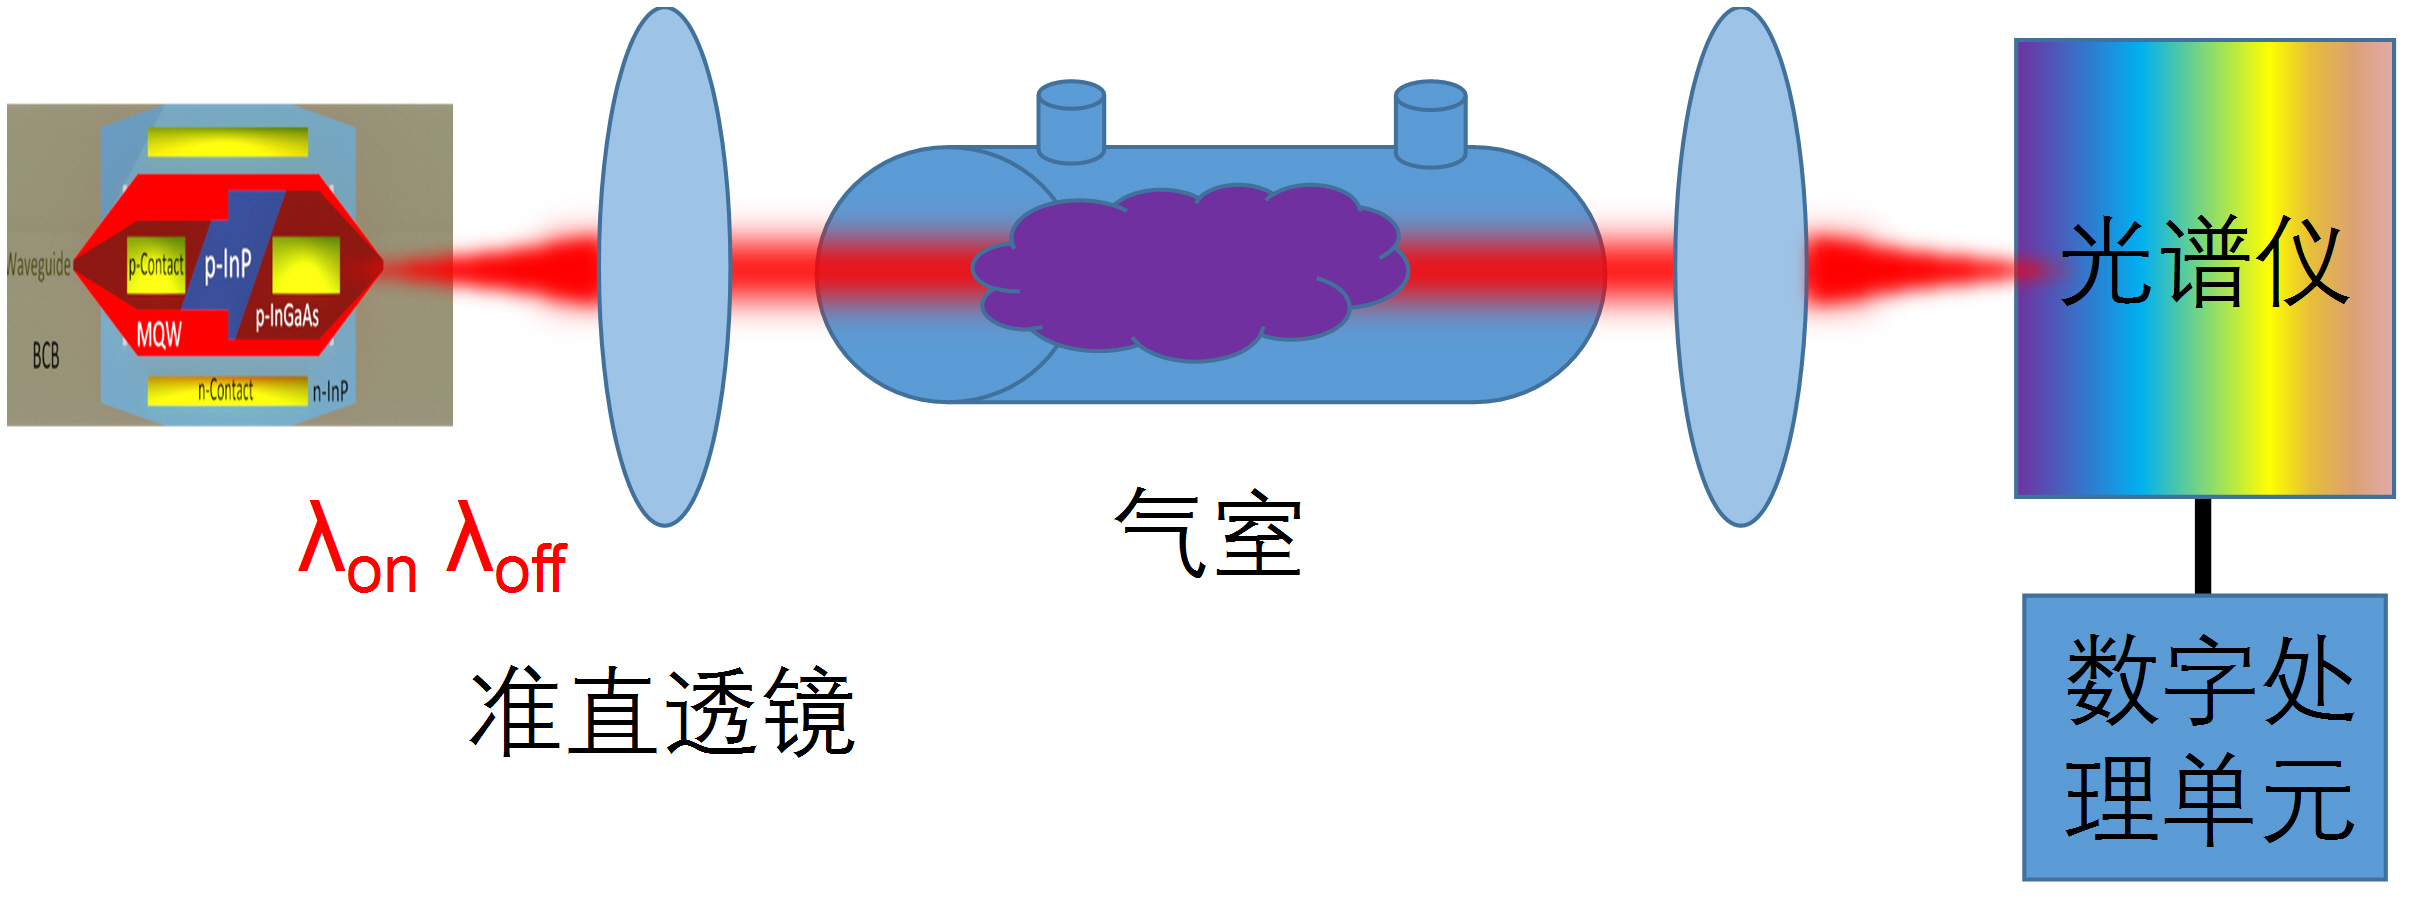
\includegraphics[width=14cm]{./Pictures/edg_gas_equipment.jpg}
	\captionsetup{justification=centering}
	\caption{非色散红外吸收光谱法检测气体浓度系统}
	\label{edg_gas_equipment}
\end{figure}

\section{片上光谱仪简介}
光谱仪在化学与生物传感,物质成分分析,光源特性标定,气体浓度测定等方面具有极其重要的作用\cite{redding2013compact}。由于传统光谱仪体积庞大,价格昂贵,无法实现便携式的测量。为此,实现片上高分辨率光谱仪对于轻便的、低价的测量具有非常重要的意义。片上光谱仪有多种实现方案:

\begin{figure}[htb]
	\centering
	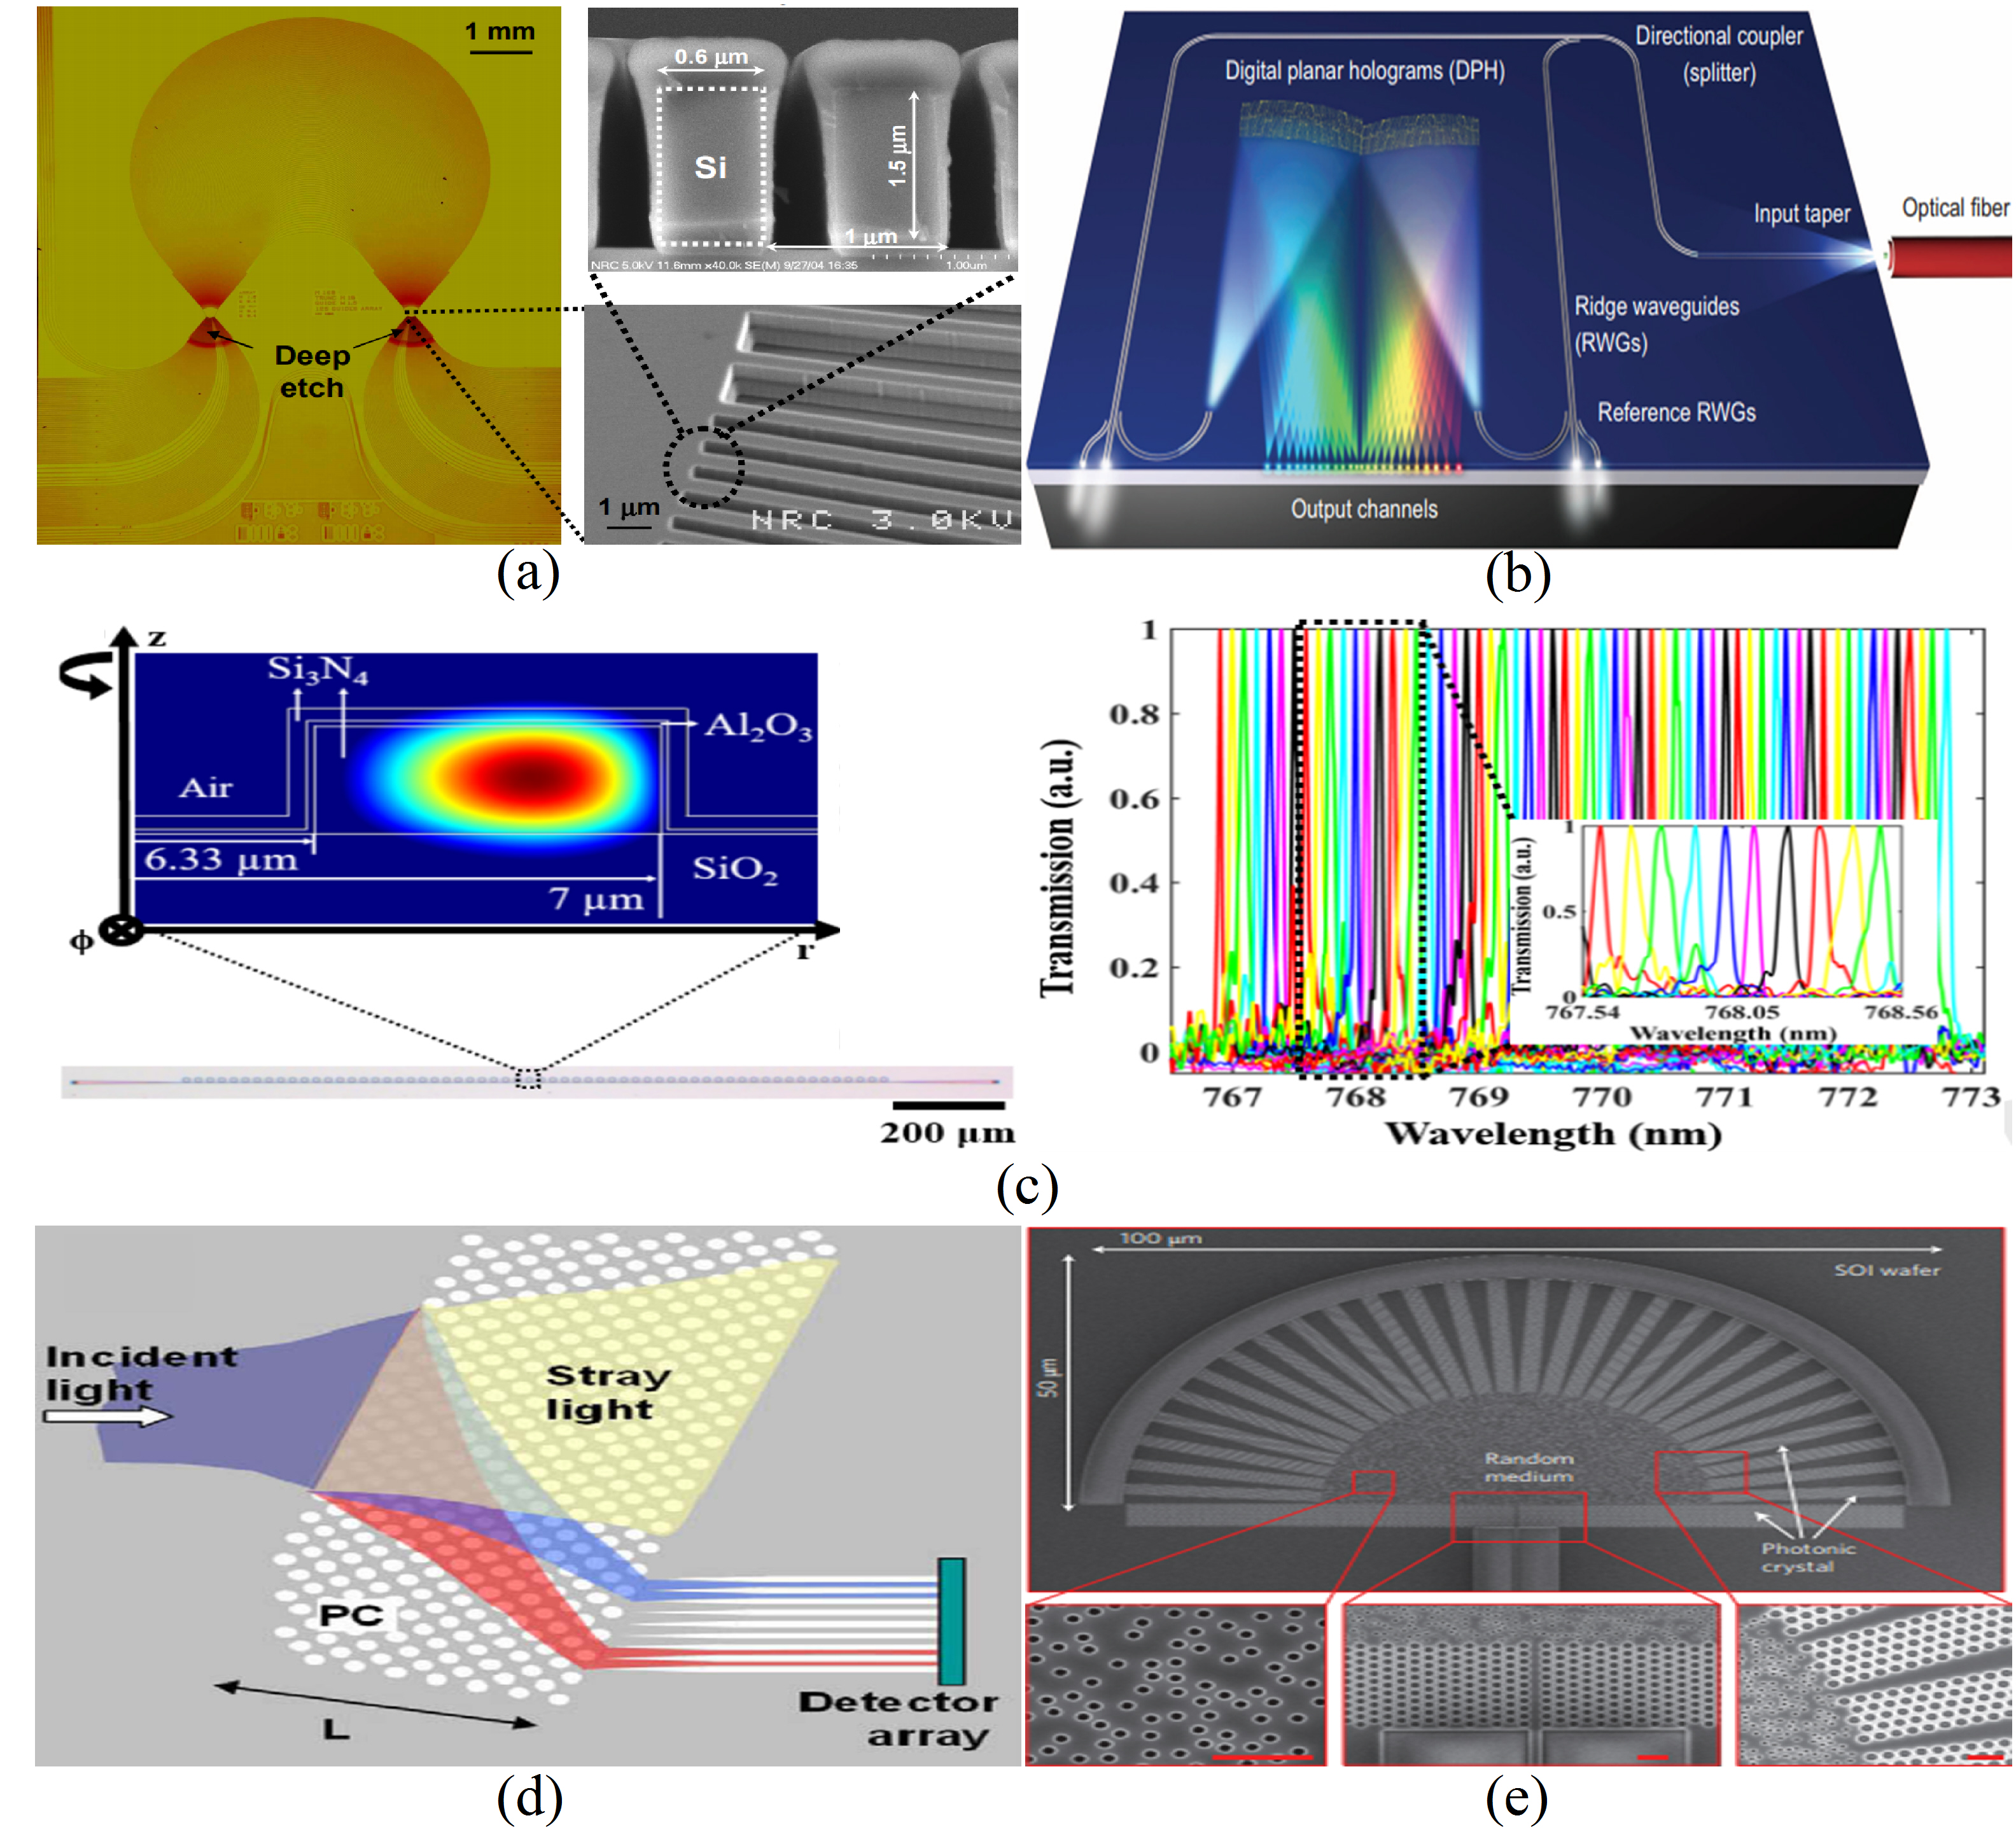
\includegraphics[width=15cm]{./Pictures/edg_background.jpg}
	\captionsetup{justification=centering}
	\caption{片上光谱仪的实现方案:(a)基于AWG的片上光谱仪\cite{cheben2007high};(b)基于数字平面全息术的片上光谱仪;(c)基于微环谐振腔的片上光谱仪\cite{fan2018highly};(d)基于光子晶体的片上光谱仪\cite{momeni2009integrated};(e)基于随机散射的片上光谱仪\cite{redding2013compact}}
	\label{edg_background}
\end{figure}

1. 基于光栅的光谱仪利用光栅对光的色散能力来实现对光谱的分离。光栅的色分辨本领正比于光栅级次m和光栅线数N,但是对于光栅来讲,光谱级次受到$d/\lambda$限制($d$为光栅周期),一般不能够很大,但光栅数可以做到很大,从而可以拥有较高的分辨率。光栅式光谱仪的光谱分辨率因此受到器件尺寸的影响,往往为了获得更高的分辨率,器件的尺寸就需要做的更大。该类片上光谱仪主要有基于阵列波导光栅(arrayed waveguide grating, AWG)和刻蚀衍射光栅(etched diffraction grating, EDG)两类。对于基于AWG与EDG的光谱仪来说,可以通过提高干涉级次或者增加阵列波导数目(AWG)、反射光栅数目(EDG)来提高光谱仪的分辨率,当光谱仪的分辨本领由于受限于输出波导之间的串扰还没有到极限的时候,还可以通过减小输出孔径的大小来提高光谱仪的分辨率。为了增加光谱仪的干涉级次,我们可以增加器件的尺寸或者选取有较高群折射率的波导\cite{matos2006arrayed}。但是增加干涉级次也会导致AWG的FSR变小,使得光谱仪的工作波长范围受到限制。所以,为了提高基于AWG与EDG的光谱仪的分辨率,减小输出孔径的尺寸会显得尤其重要。图\ref{edg_background}(a)展示了一个基于AWG的光谱仪,器件尺寸为8~$mm$~$\times$~8~$mm$,分辨率0.2~$nm$,通道数为50\cite{cheben2007high},该AWG连接自由传输区(free propagation region, FPR)的输出波导尺寸为1.5~$\mu m~\times$~0.6~$\mu m$,实现了亚波长的波导间距,但由于该波导结构的硅层厚度达到1.5~$\mu m$,与常用的SOI芯片并不匹配。

2. 利用数字平面全息术(digital planar holography, DPH)可以用来制作光谱仪\cite{peroz2012multiband}。平面全息术利用特殊设计的几百万条线型结构来实现对特定波长的分离,这些位结构通过构成布拉格反射镜,聚焦椭圆反射镜,并且该结构可以利用全息术的影像叠加效应,周期结构的禁带效应来实现对光传播的控制。可以这样理解,数字平面全息术可以将任意光学传递函数编码到一个平面器件当中,从而在频域和空域上将不同波长的光波进行分离。该类型光谱仪可以实现与传统光谱仪相比拟的性能,根据所需工作波长,选择不同的材料平台来实现,在可见光波段可以使用SiO\SB{2}Ge\SB{x},HfO\SB{2}或者Si\SB{3}N\SB{4},近红外可以使用Si或者Si\SB{3}N\SB{4}。图\ref{edg_background}(b)展示了Calafiore等人利用该原理实现了近红外分辨率0.15~$nm$的分辨率且带宽范围为148~$nm$,器件的尺寸小于2~$cm$\SP{2}\cite{calafiore2014holographic}。该方案的缺点是需要专门开发的算法来优化制作的全息光栅,否则会导致模式泄漏到包层模,光栅的二阶反射,输出通道的互相干扰等问题。而且还有个问题就是该类型的光谱仪由于损耗较大,故灵敏度会比较低。

3. 谐振腔型的光谱仪可以使得有效光程远远大于实际的器件尺寸,从而可以在较小的尺寸里实现超高的分辨率。常用的用来制作光谱仪的谐振结构有微环,光子晶体谐振腔。但是该类型光谱仪对制作误差非常敏感,通道的波长需要进行后期校准。图\ref{edg_background}(c)展示了Tianren等人在Si\SB{3}N\SB{4}平台上利用60个微环阵列实现了100~$pm$的光谱分辨率,波长范围为6~$nm$,并利用后期校准技术实现了所有通道波长漂移量标准差只有5~$pm$\cite{fan2018highly}。

4. 光子晶体具有非常强的色散效应,因此可以利用它来实现光谱的分离,它可以在很小的尺寸下获得较高的分辨率,因此非常利于集成。Babak等人利用光子晶体的负衍射效应,将信号光与杂散光分离并聚焦到对应的通道上,实现不同波长光的分离,如图\ref{edg_background}(d)所示。该结构在SOI上制作,器件尺寸为80~$\mu m~\times~220~\mu m$,利用一些校正的方法,可以在50~$nm$范围内实现10~$pm$的分辨率,但是该光谱仪的缺点是只能用来探测单一的谱线\cite{momeni2009integrated}。

5. 图\ref{edg_background}(e)展示了一种利用随机散射来实现的光谱仪,在25~$\mu m~\times~50~\mu m$的尺寸里实现了0.75~$nm$的分辨率,带宽25~$nm$\cite{redding2013compact}。该器件的原理是,不同波长的输入光经过杂乱的系统会形成不同的模斑,将这些模斑记录下来,通过校准,就可以反过来通过输入信号形成的模斑来反推出输入信号的光谱。由于光在杂乱的系统中需要经过多次反射,大大增加了光程,所以能够在较小的器件尺寸下实现较高的分辨率。该光谱仪还有一个优点是可以用同一个结构,实现不同光谱范围的探测,只需要做相应的校准即可。

表\ref{spectrometer_summary}对以上片上光谱仪方案做了总结。
\begin{table}[htb]
	\zihao{5}
	\captionsetup{justification=centering}
	\caption{不同类型光谱仪特性总结}
	\label{spectrometer_summary}
	\centering
	\begin{tabular}[t]{|ccc|}
		\hline
		\textbf{光谱仪类型} & \textbf{优点} & \textbf{缺点}  \\
		\hline
		光栅型光谱仪(AWG,EDG)&设计成熟、工艺方便&尺寸较大\\
		\hline
		数字平面全息光谱仪&分辨率较高&损耗较大,灵敏度受限\\
		\hline
		谐振腔型光谱仪&分辨率高,尺寸较小&对工艺敏感,需后期校正\\
		\hline
		光子晶体光谱仪&分辨率高,尺寸较小&只能用来探测单一的谱线\\
		\hline
		随机散射光谱仪&分辨率高,波长范围可切换&需要专门的算法优化\\
		\hline
	\end{tabular}
\end{table}

\section{基于EDG光谱仪的设计优化}
\subsection{输出波导阵列的优化}
为了提高基于EDG的光谱仪在尺寸固定下的分辨率,从上一节的背景研究了解到,我们可以利用密集波导阵列来减小输出孔径的大小。密集波导阵列首先在模式复用方面获得了应用\cite{liu2015densely,chen2015experimental},提高了模式复用器件的集成度。与此类似,我们首先提出尝试将密集波导阵列应用于EDG,分光能力的情况下,提高光谱仪的分辨率,或者在相同分辨率的情况下,我们可以利用密集阵列波导作为输出波导实现更小的器件尺寸。

最简单的密集波导阵列由两根波导组成,两根波导之间的耦合可以用公式\ref{coupling_two_waveguides}来表示\cite{saleh1991fundamentals}:
\begin{equation}
\label{coupling_two_waveguides}
\dfrac{P_{1\rightarrow2}}{P_{1}}=\frac{1}{(\Delta\beta /2\kappa)^2+1}sin^2\sqrt{(\Delta \beta/2)^2 +\kappa^2}L
\end{equation}
其中$\Delta \beta$代表两根波导的传播常数之差,$\kappa$是两根波导之间的耦合系数,$L$是耦合长度。从中我们可以看到,最大的耦合强度$max[P_{1\rightarrow2}/P_{1}]$为$1/[(\Delta\beta/2\kappa)^2 +1]$,所以为了减小两根波导之间的串扰,我们只需要让两根波导相位失配足够严重,即$\Delta\beta>>\kappa$,就能让两根波导的串扰足够小。但是,如果由两根波导组成波导阵列,阵列波导的密度也不能太高,因为靠的较近的两根相同宽度的波导在距离不够大的时候比较容易发生耦合从而导致较高的串扰\cite{song2015high}。所以,为了实现密集波导阵列,光研究两根波导之间的耦合是远远不够的。

密集波导阵列的设计思路如下,首先我们需要设计一个最小基本单元,使得在该单元内不同波导之间的串扰足够小。然后将这个最小单元扩展,形成阵列,使得低串扰依然能够保持。为了实设计最小的基本单元,通过类比的方法,我们可以将该基本单元看成一个“分子”,我们需要找出组成这个“分子”的“原子”,对于波导来说,实现不同的“原子”最简单的方法就是用不同的宽度的波导,因为这在集成平面光波导加工工艺中最容易实现,如果要用不同厚度的波导,会给工艺增加不必要的难度。在常用的220~$nm$~SOI平台上,波导宽度的选取受到两点限制:1,波导宽度不能太大,否则会产生高阶模式,增加波导阵列之间的耦合。2,波导宽度不能太小,因为当波导宽度减小到一定程度,模式的宽度反而会变大,导致波导之间的耦合增强,而且波导宽度越小,模式受到波导侧壁的影响就会越大,波导的侧壁往往因为刻蚀而比较粗糙,故损耗也会增加。这两个方面限制了我们选取波导宽度的范围。

\begin{figure}[htb]
	\centering
	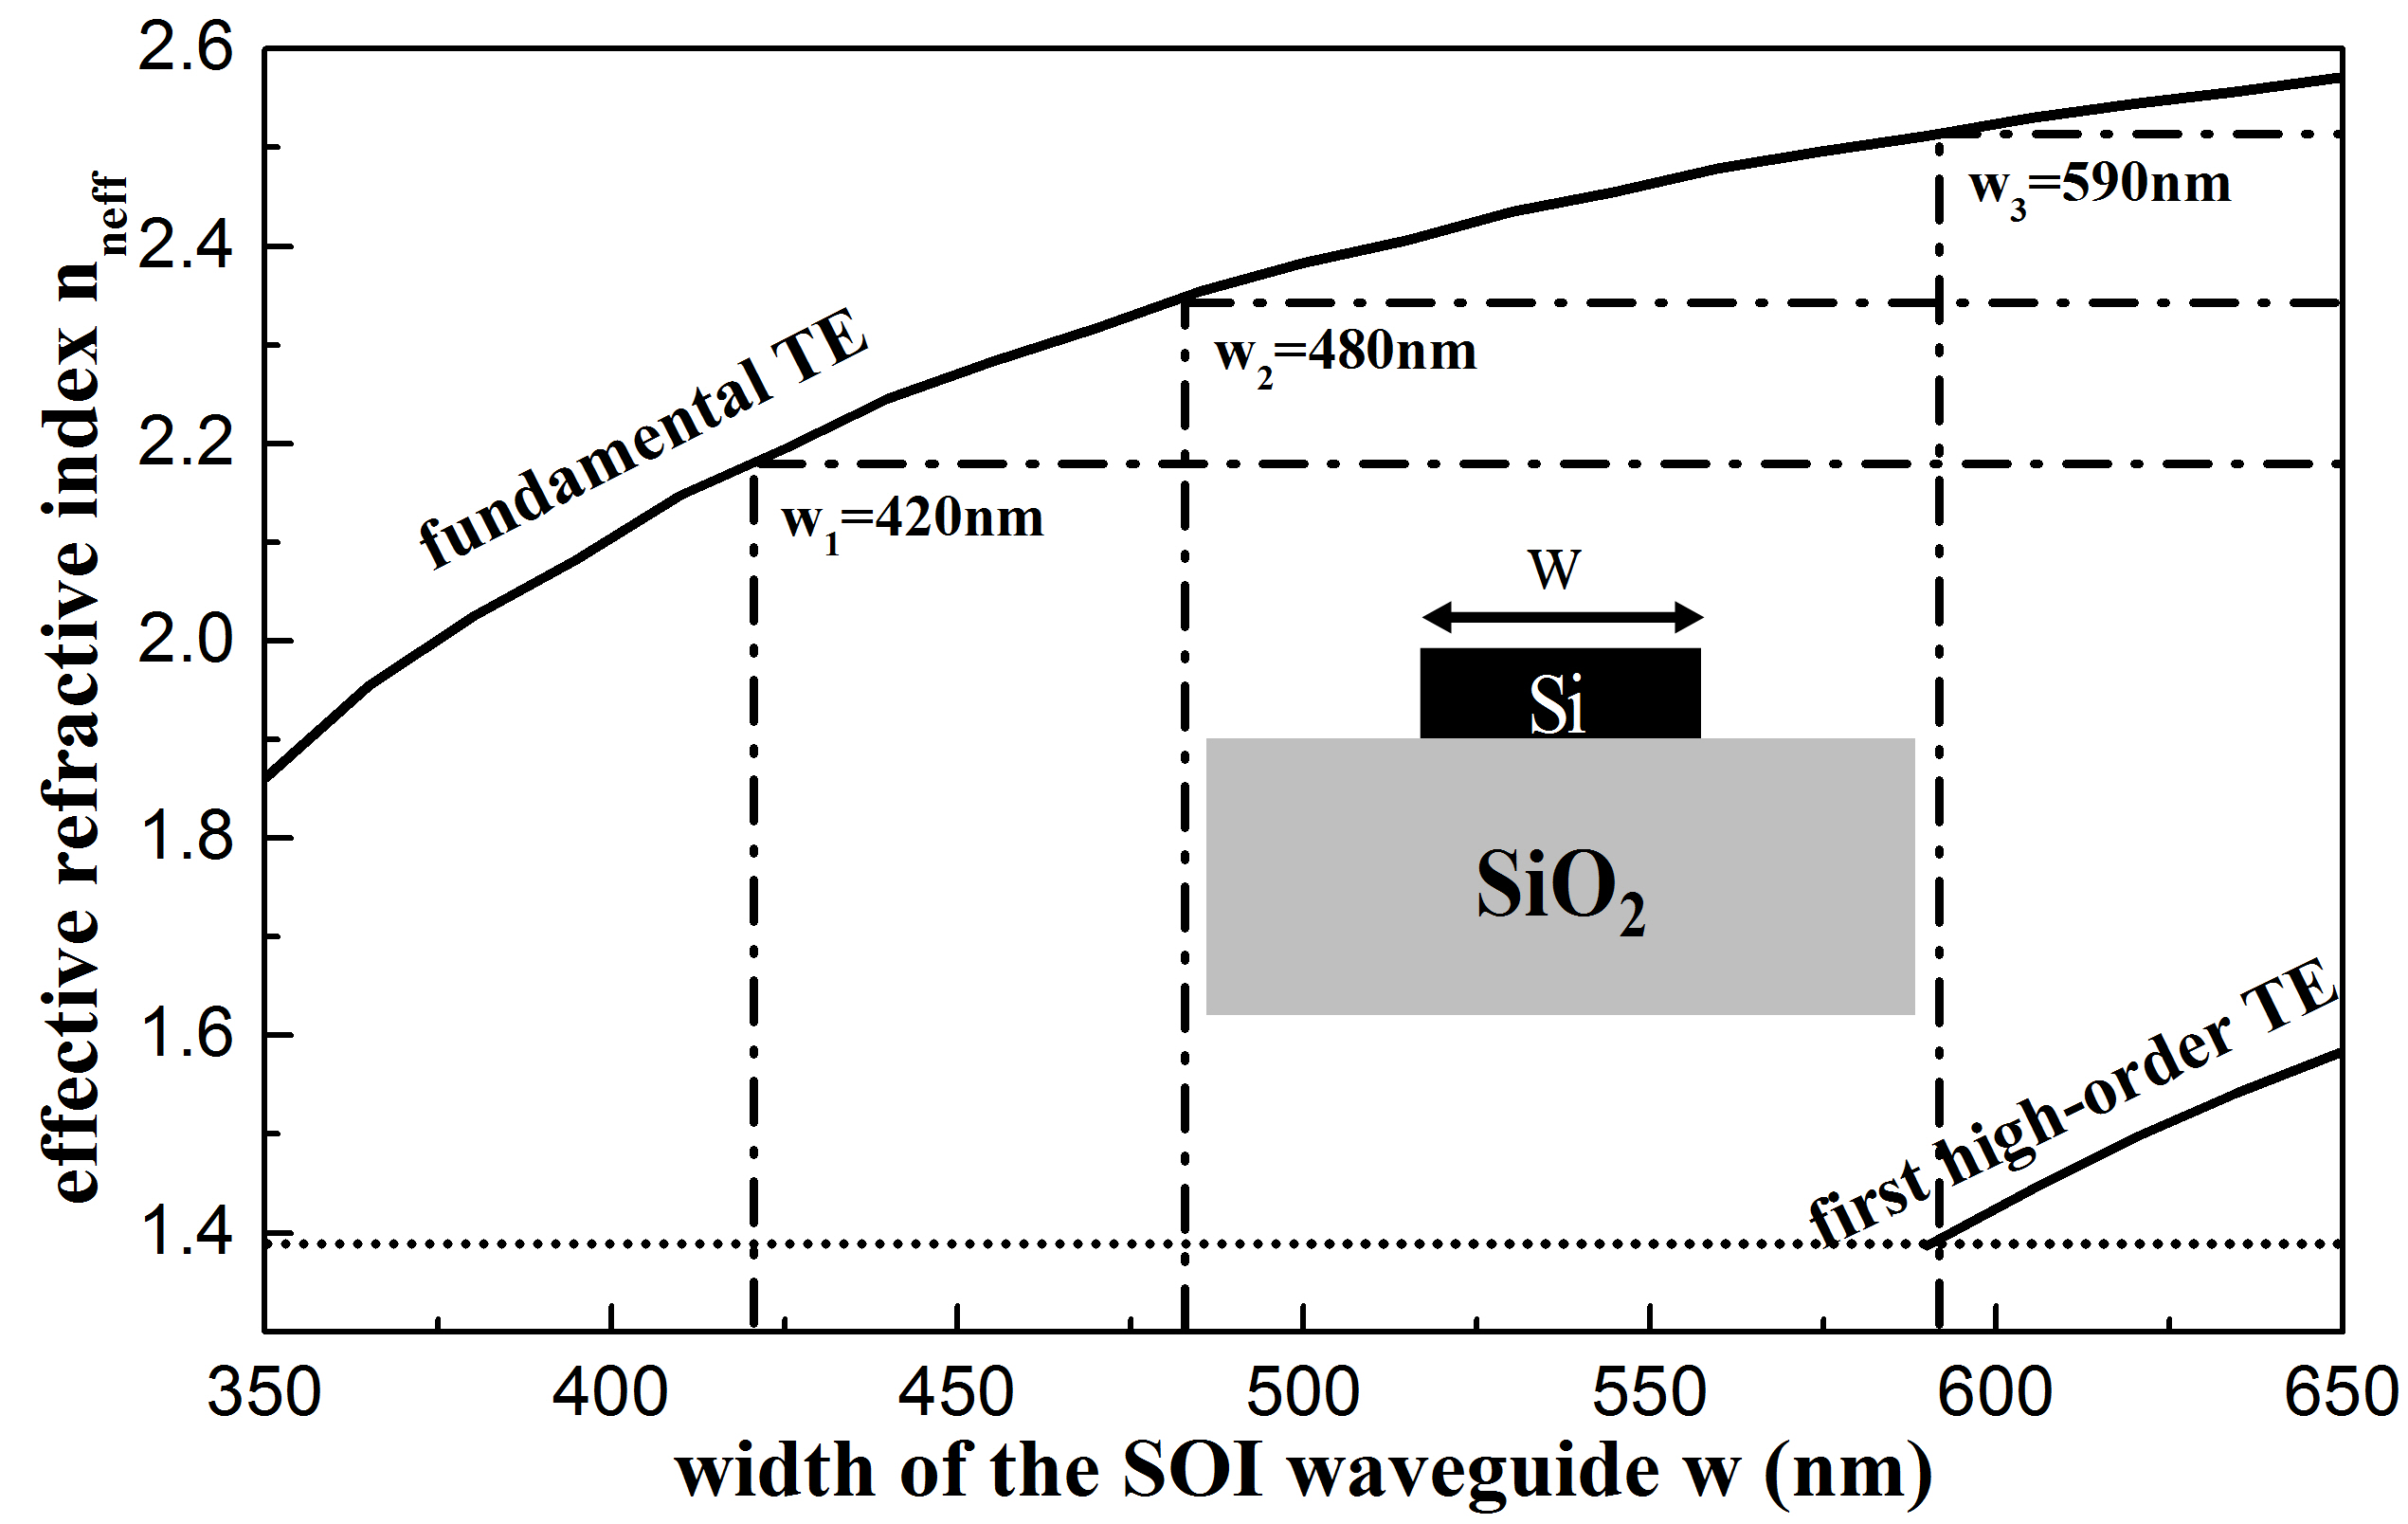
\includegraphics[width=14cm]{./Pictures/edg_refractive_index.jpg}
	\captionsetup{justification=centering}
	\caption{不同宽度波导的模式等效折射率$n_{eff}$,波导的高度为220~$nm$,工作波长为1550~$nm$}
	\label{edg_refractive_index}
\end{figure}

我们用Lumerical~MODE~Solutions\cite{modesolution}仿真计算了220~$nm$~SOI平台的波导等效折射率与波导宽度之间的关系,如图\ref{edg_refractive_index}所示。当波导宽度大于590~$nm$时,会出现TE高阶模,故我们选取的波导最大宽度为590~$nm$。根据我们实验室的工艺经验,波导宽度小于400~$nm$时,波导损耗会快速增加,故我们选择波导最小宽度为420~$nm$,留出一些余量。选定了波导宽度范围之后,我们先选取组成“分子”的“原子”数目为3,这也是为了尽量减小系统的复杂度,3个“原子”的宽度分别为w\SB{1}~=~420~$nm$,w\SB{2}~=~480~$nm$,w\SB{3}~=~590~$nm$,这样取是为了让不同“原子”间的等效折射率差达到最大,从而它们之间的相位失配达到最大,串扰就能达到最小。如果“原子”数目增多,势必会减小不同“原子”之间的相位失配度,使得串扰会有所增大。

\begin{figure}[htb]
	\centering
	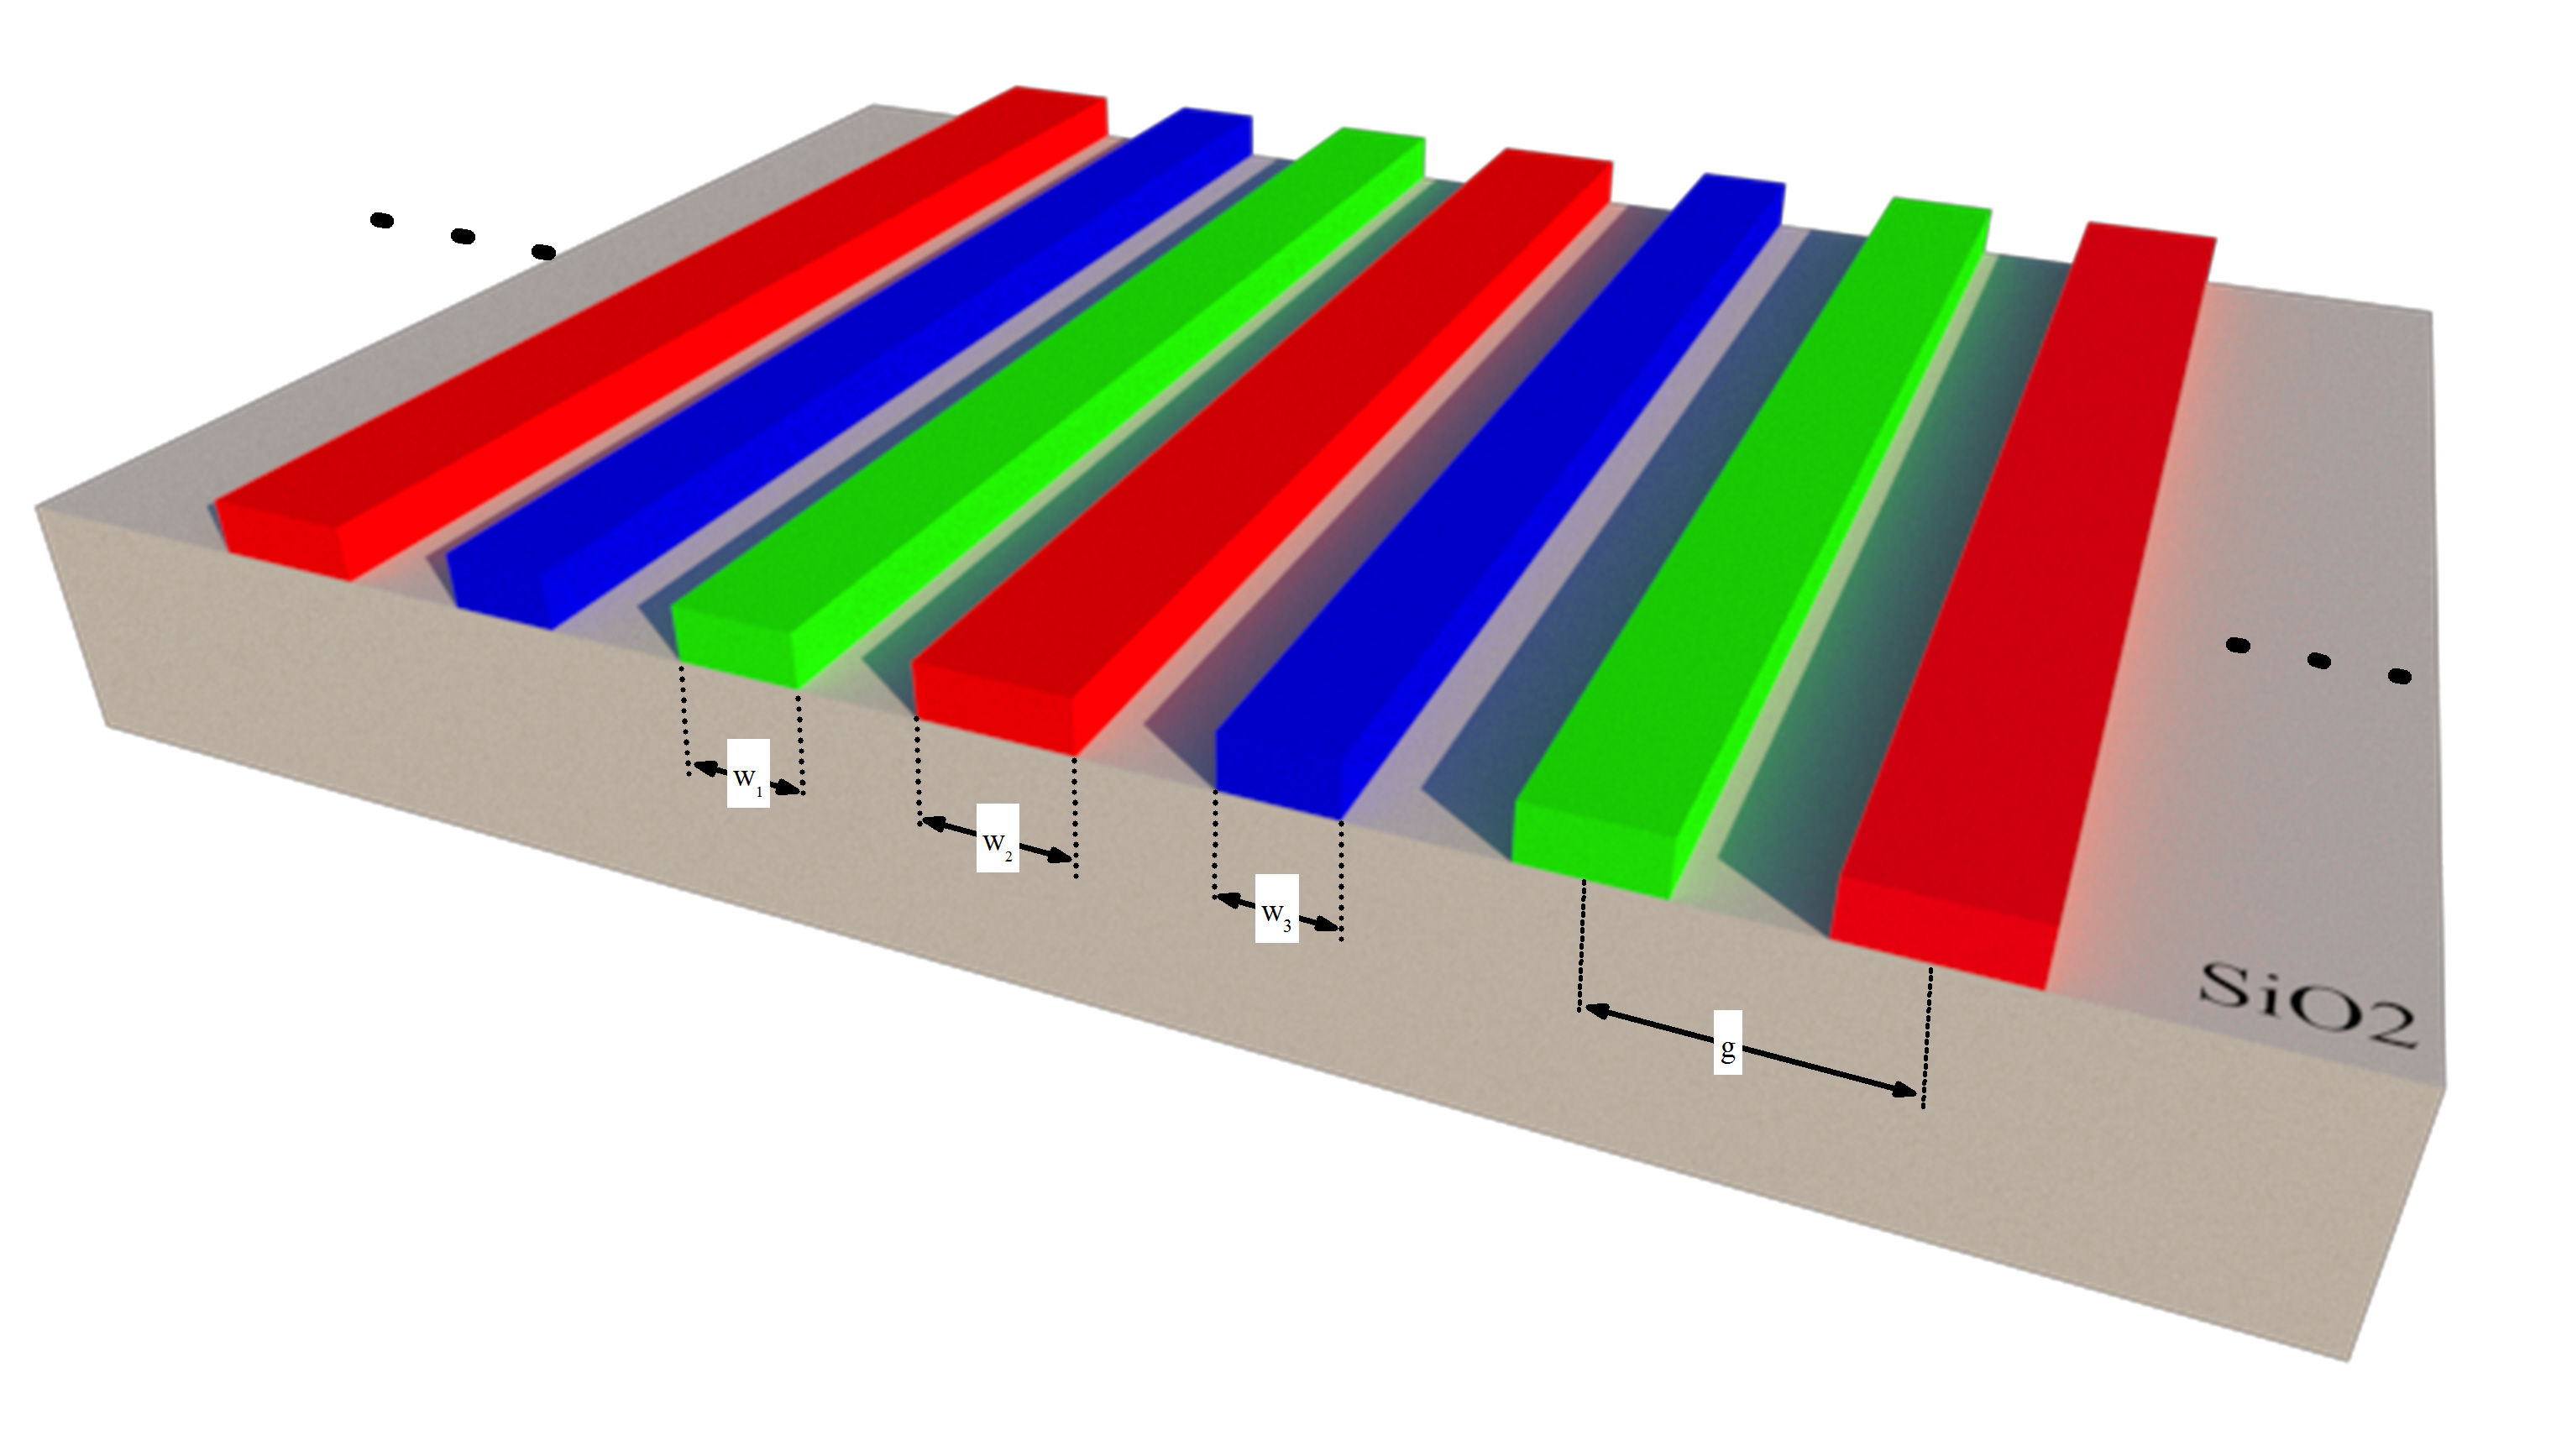
\includegraphics[width=14cm]{./Pictures/edg_dpwg.jpg}
	\captionsetup{justification=centering}
	\caption{波导阵列3D示意图,w\SB{1}~=~420~$nm$,w\SB{2}~=~480~$nm$,w\SB{3}~=~590~$nm$,g~=1~$\mu m$}
	\label{edg_dpwg}
\end{figure}

我们设计的波导阵列示意图如图\ref{edg_dpwg}所示,图中只画出了波导阵列的一部分,不同颜色的波导宽度不同,其中w\SB{1}~=~420~$nm$,w\SB{2}~=~480~$nm$,w\SB{3}~=~590~$nm$,波导间距g~=1~$\mu m$。从中我们可以看到,3种不同宽度的波导作为基本单元,然后有这些基本单元组成类似超晶格的结构。考虑串扰时,我们将其分为两个层次,首先考虑基本单元内部的串扰,之后再考虑不同单元间的串扰。

我们用Lumerical~FDTD~Solutions\cite{fdtdsolution}仿真了两根相同宽度的波导之间的串扰如图\ref{edg_xtalk_no_taper}(a)所示,波导宽度为500~$nm$,间距为1~$\mu m$,当传输距离为50~$\mu m$时,串扰约为-17~dB。与之相对,当采用上述设计的密集波导阵列时,结果如图\ref{edg_xtalk_no_taper}(b)所示,在波导阵列中传输的模式串扰在100~$nm$带宽范围内均小于-50~dB,传输长度也为50~$\mu m$,能够实现很好的独立传输性能。此处仿真只考虑了模式在传输过程中的串扰,忽略了模式的激发问题。

\begin{figure}[htb]
	\centering
	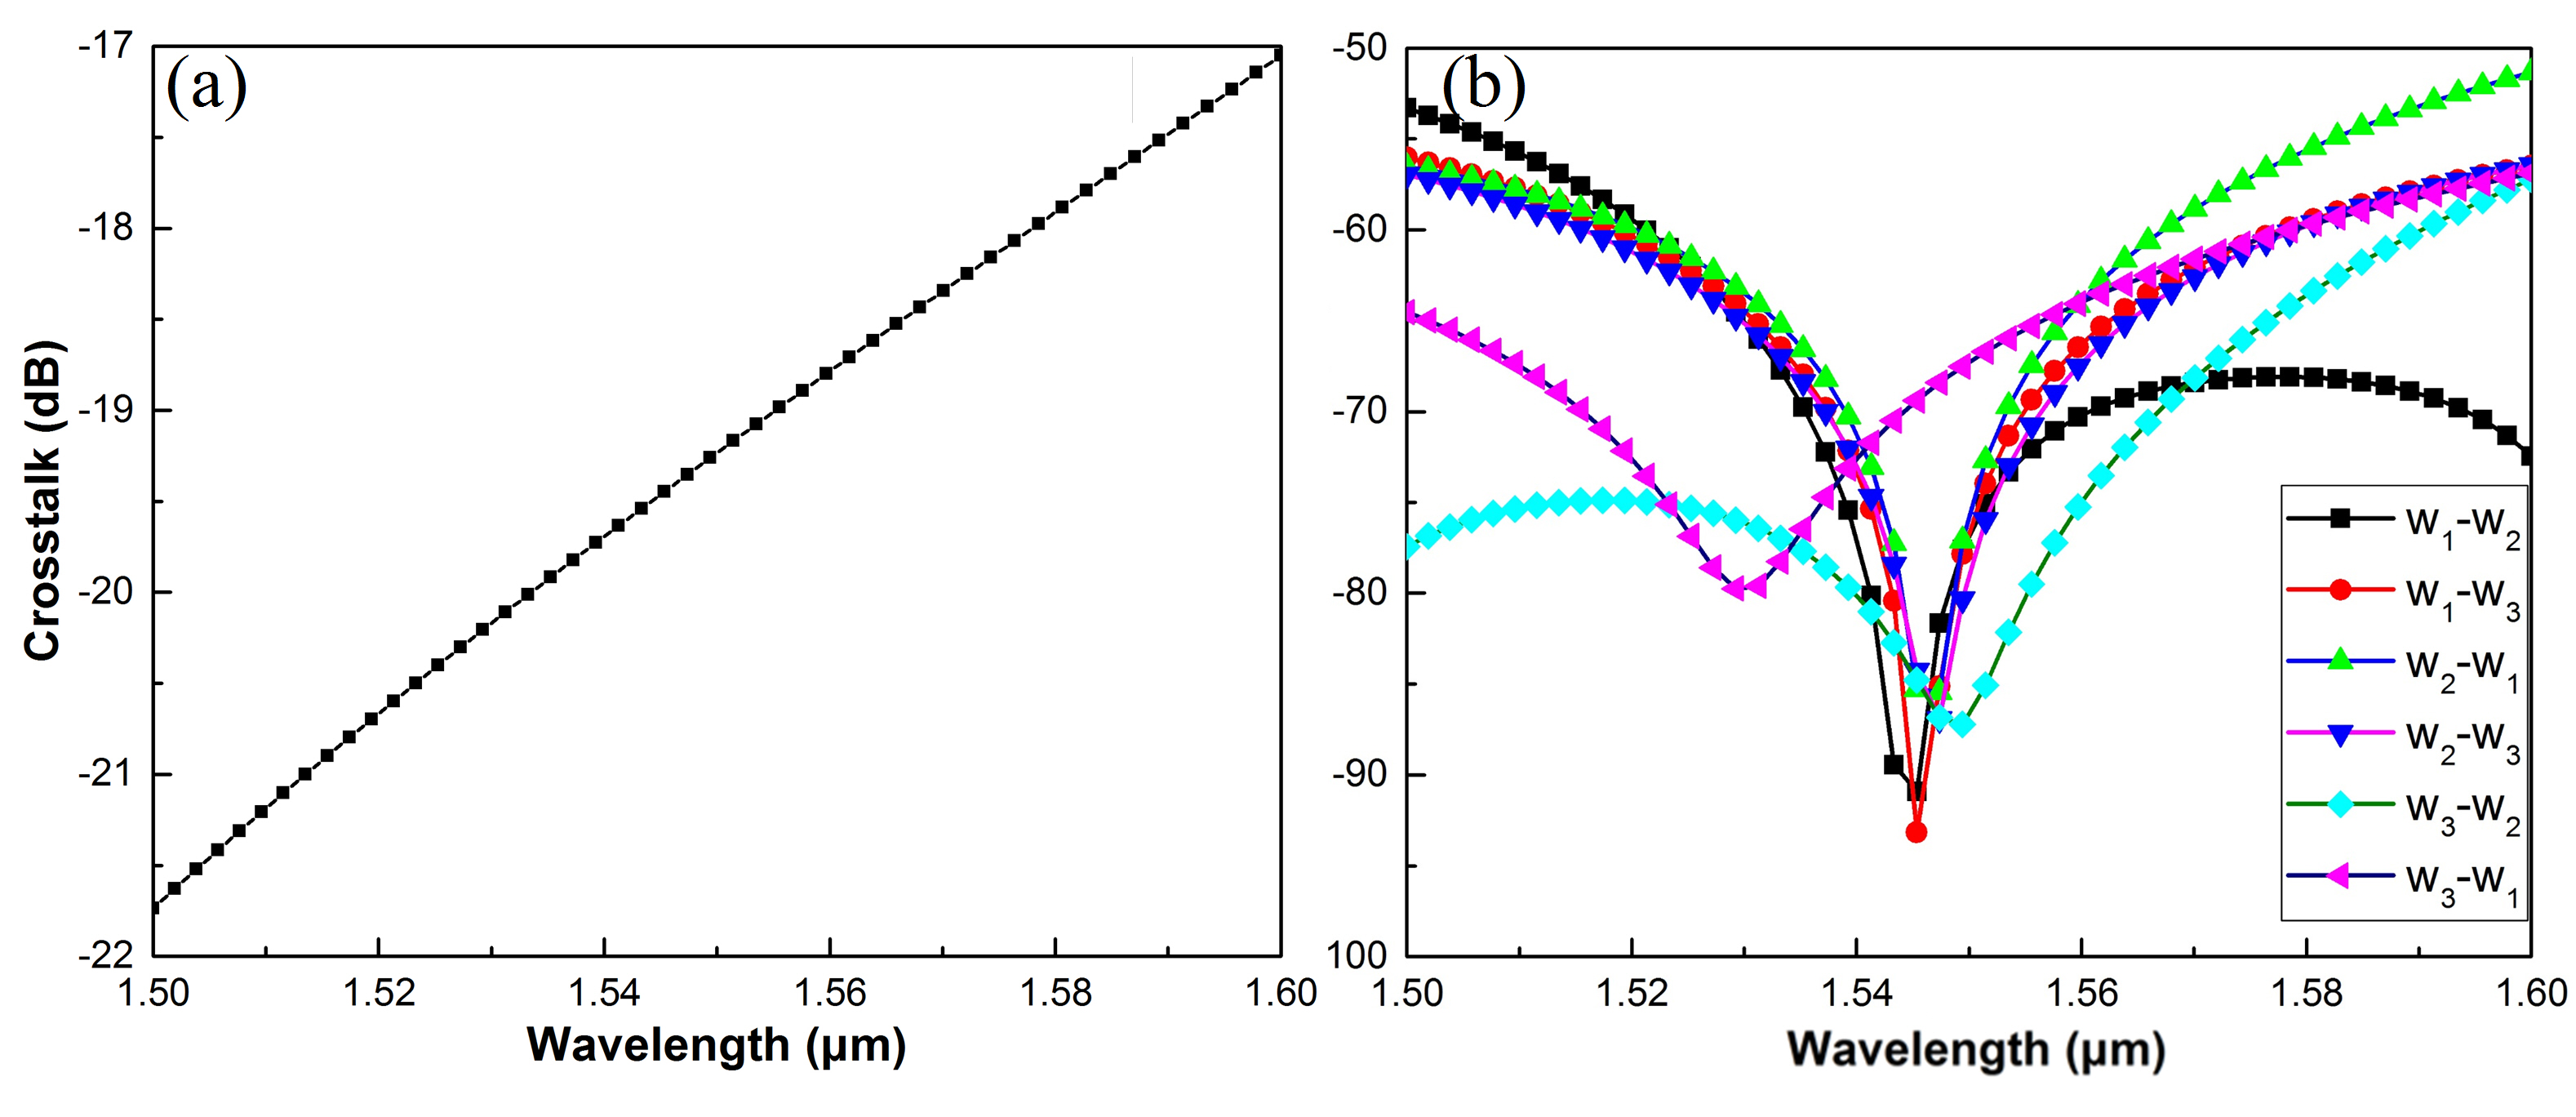
\includegraphics[width=16cm]{./Pictures/edg_xtalk_no_taper.jpg}
	\captionsetup{justification=centering}
	\caption{(a)两根宽度为500~$nm$的波导在传输50~$\mu m$之后的串扰;(b)密集波导阵列中相邻波导之间的串扰,w\SB{1}-w\SB{2}表示宽度为w\SB{1}的波导中的模式耦合到宽度为w\SB{2}的波导中的串扰,w\SB{1}~=~420~$nm$,w\SB{2}~=~480~$nm$,w\SB{3}~=~590~$nm$}
	\label{edg_xtalk_no_taper}
\end{figure}

\begin{figure}[htb]
	\centering
	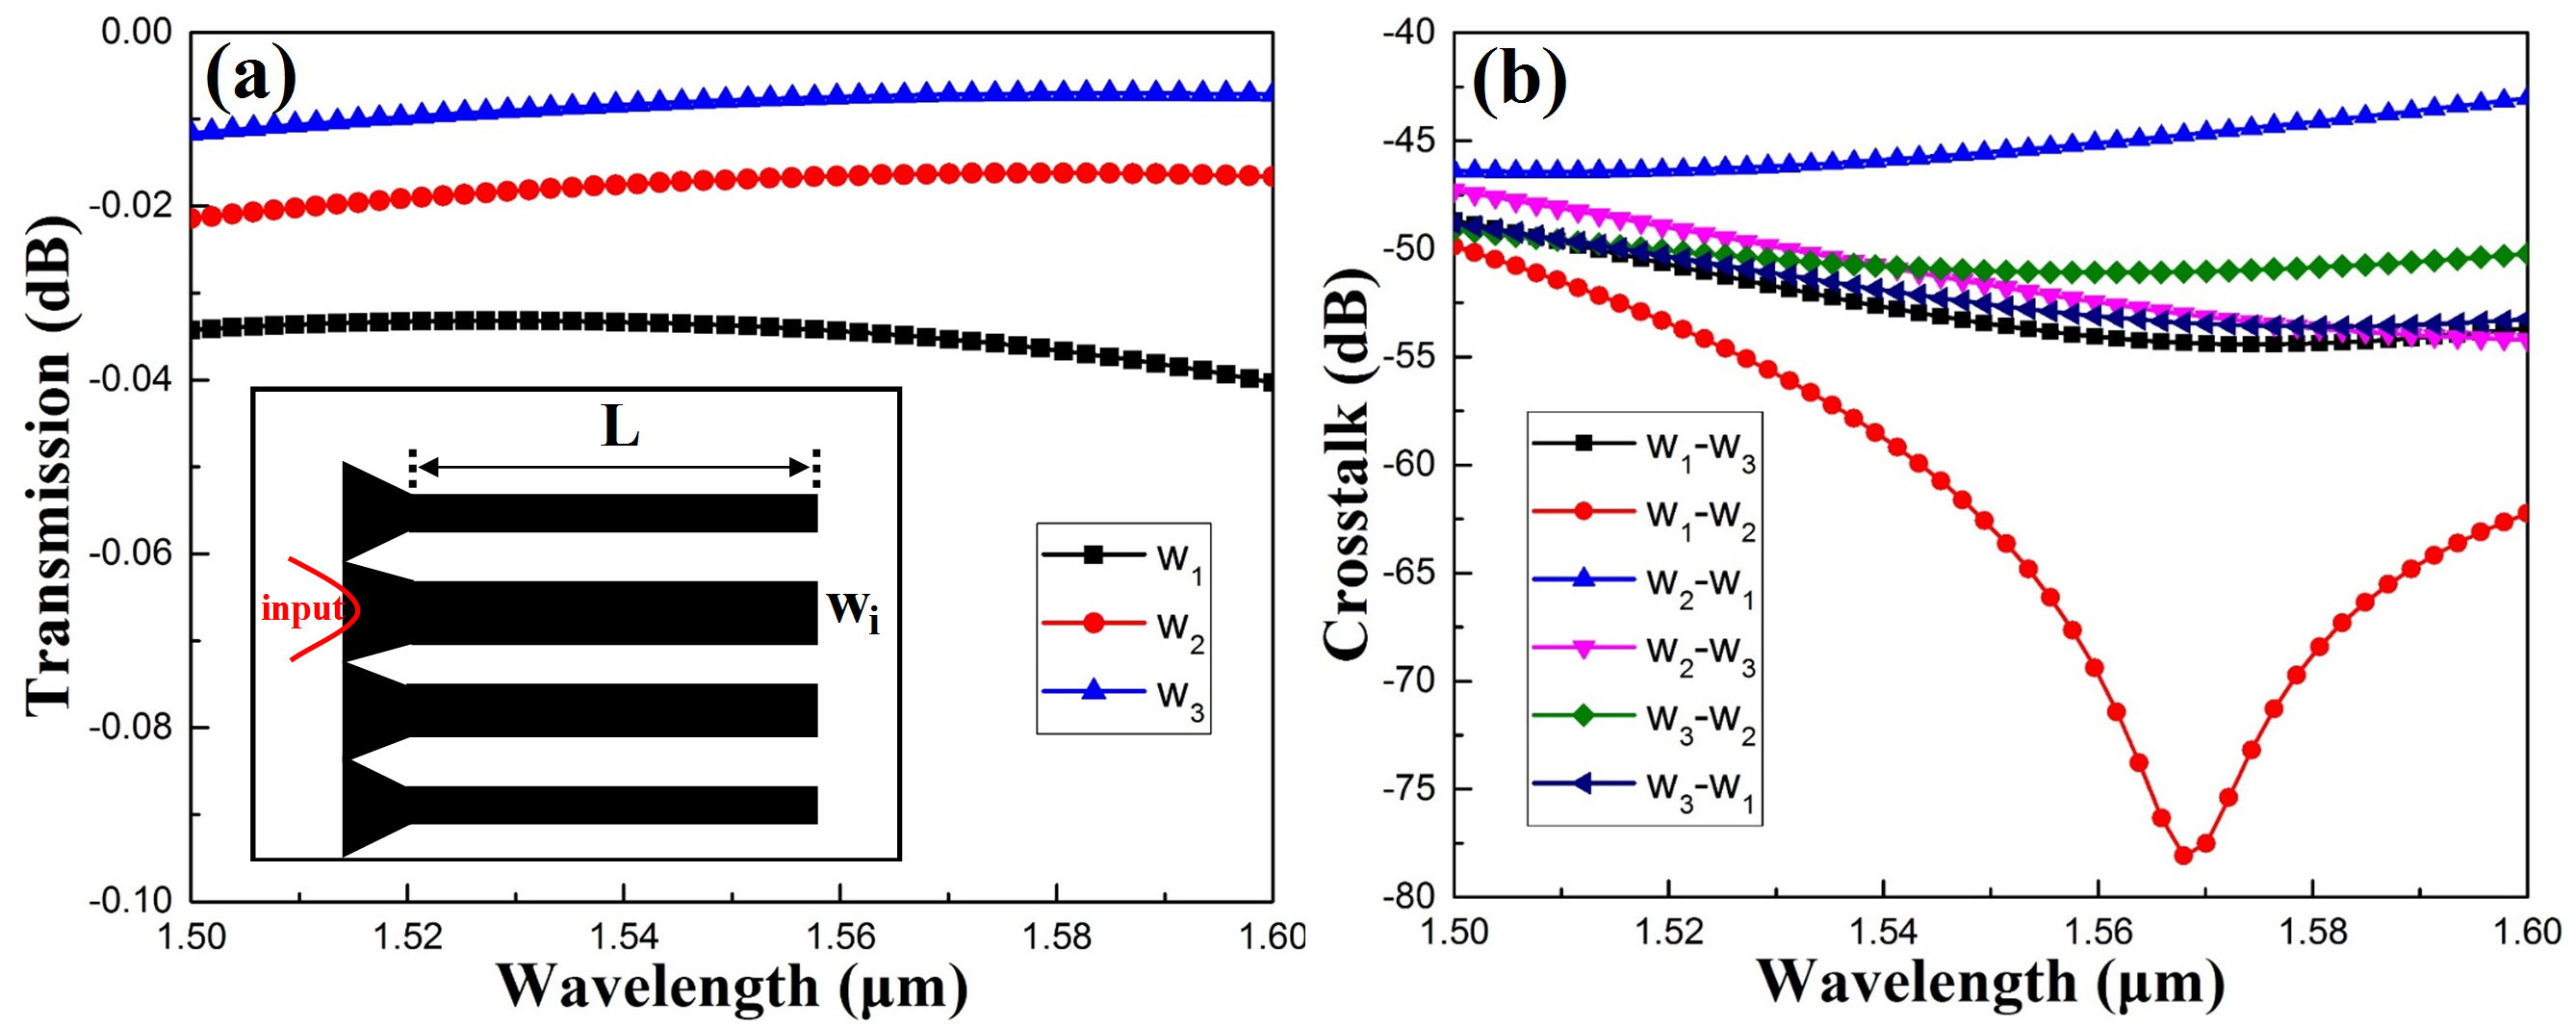
\includegraphics[width=16cm]{./Pictures/edg_taper_xtalk.jpg}
	\captionsetup{justification=centering}
	\caption{(a)~800~$nm$波导渐变到不同宽度波导的插损,插图为所使用的仿真模型,L~=~50~$\mu m$;(b)包含锥形波导结构之后相邻波导之间的串扰,$w_{1}$~=~420~$nm$,$w_{2}$~=~480~$nm$,$w_{3}$~=~520~$nm$}
	\label{edg_taper_xtalk}
\end{figure}

考虑到波导阵列的宽度不一样,如果直接将它们作为输出口,每个通道接收到的能量必然将不同,从而使得光谱仪的通道均匀性受到影响。故我们在输出波导入口处增加一个锥形波导结构,将3种不同宽度的波导渐变到同一个较宽的宽度,同时也可以减小光谱仪的插入损耗。我们将锥形波导入口处的宽度设为800~$nm$,由于锥形波导的长度过长会影响输出波导之间的串扰性能,故我们将其长度设为1~$\mu m$。于此同时,为了输入端口与输出端口的模式匹配,并且假设我们的光栅反射镜成像具有一比一的性质,我们将输入波导的宽度也设为800~$nm$。之后我们仿真验证了输出端口处加入该锥形波导之后基模透过率的性能,我们采用图\ref{edg_taper_xtalk}(a)中插图所示的仿真模型来计算加入锥形波导之后引入的插损与串扰特性,插损结果如图\ref{edg_taper_xtalk}(a)所示,从中可以看到,加入锥形波导引起的损耗在100~$nm$带宽范围内均小于0.05~dB。为了验证所加入的锥形波导是否会引起额外的串扰,我们仿真了有锥形波导存在的情况下不同宽度波导之间的串扰,此时光场以一根宽度为800~$nm$的波导的基模输入,经过锥形波导耦合到密集波导阵列中,通过分析相邻波导中的能量获得串扰信息,结果如图\ref{edg_taper_xtalk}(b)所示。可以看到,此时的串扰比没有锥形波导存在情况下时增加了10~dB,但总体还是在-40~dB以下,故该波导阵列可用于作为EDG的输出波导阵列。在SOI平台上,Song等人\cite{song2012chip}在220~$nm$~SOI平台上制作的EDG光谱仪输出波导间距为5~$\mu m$,Pommarede等人\cite{pommarede201716}在300~$nm$~SOI平台上制作的EDG波导间距为2.5~$\mu m$,都远远大于我们设计的波导阵列的波导间距1~$\mu m$。故在相同的分辨率要求下,我们设计的EDG可以做到更紧凑,且能够集成更多的输出通道。

\subsection{反射光栅的优化}
EDG的反射镜我们采用了分布式布拉格反射镜(distributed brag reflector, DBR),该反射镜具有反射率高,在组成折射率材料差较大的情况下,可以提供较大的带宽等优点\cite{lycett2013perfect},但是要求入射角比较小。相比较于金属反射面,可以减少工艺步骤。我们选取反射镜的周期为480~$nm$,占空比为0.5,刻蚀深度220~$nm$。周期数我们选为3,这牺牲了一定的反射率,主要是为了减少EBL的曝光时间。我们用Lumerical~FDTD~Solutions\cite{fdtdsolution}仿真得到的反射谱如图\ref{edg_dbr_loss}所示,从图中可以看到反射镜的损耗在100~nm带宽范围内均小于1.6~dB,不均匀性约为0.5~dB。

\begin{figure}[htb]
	\centering
	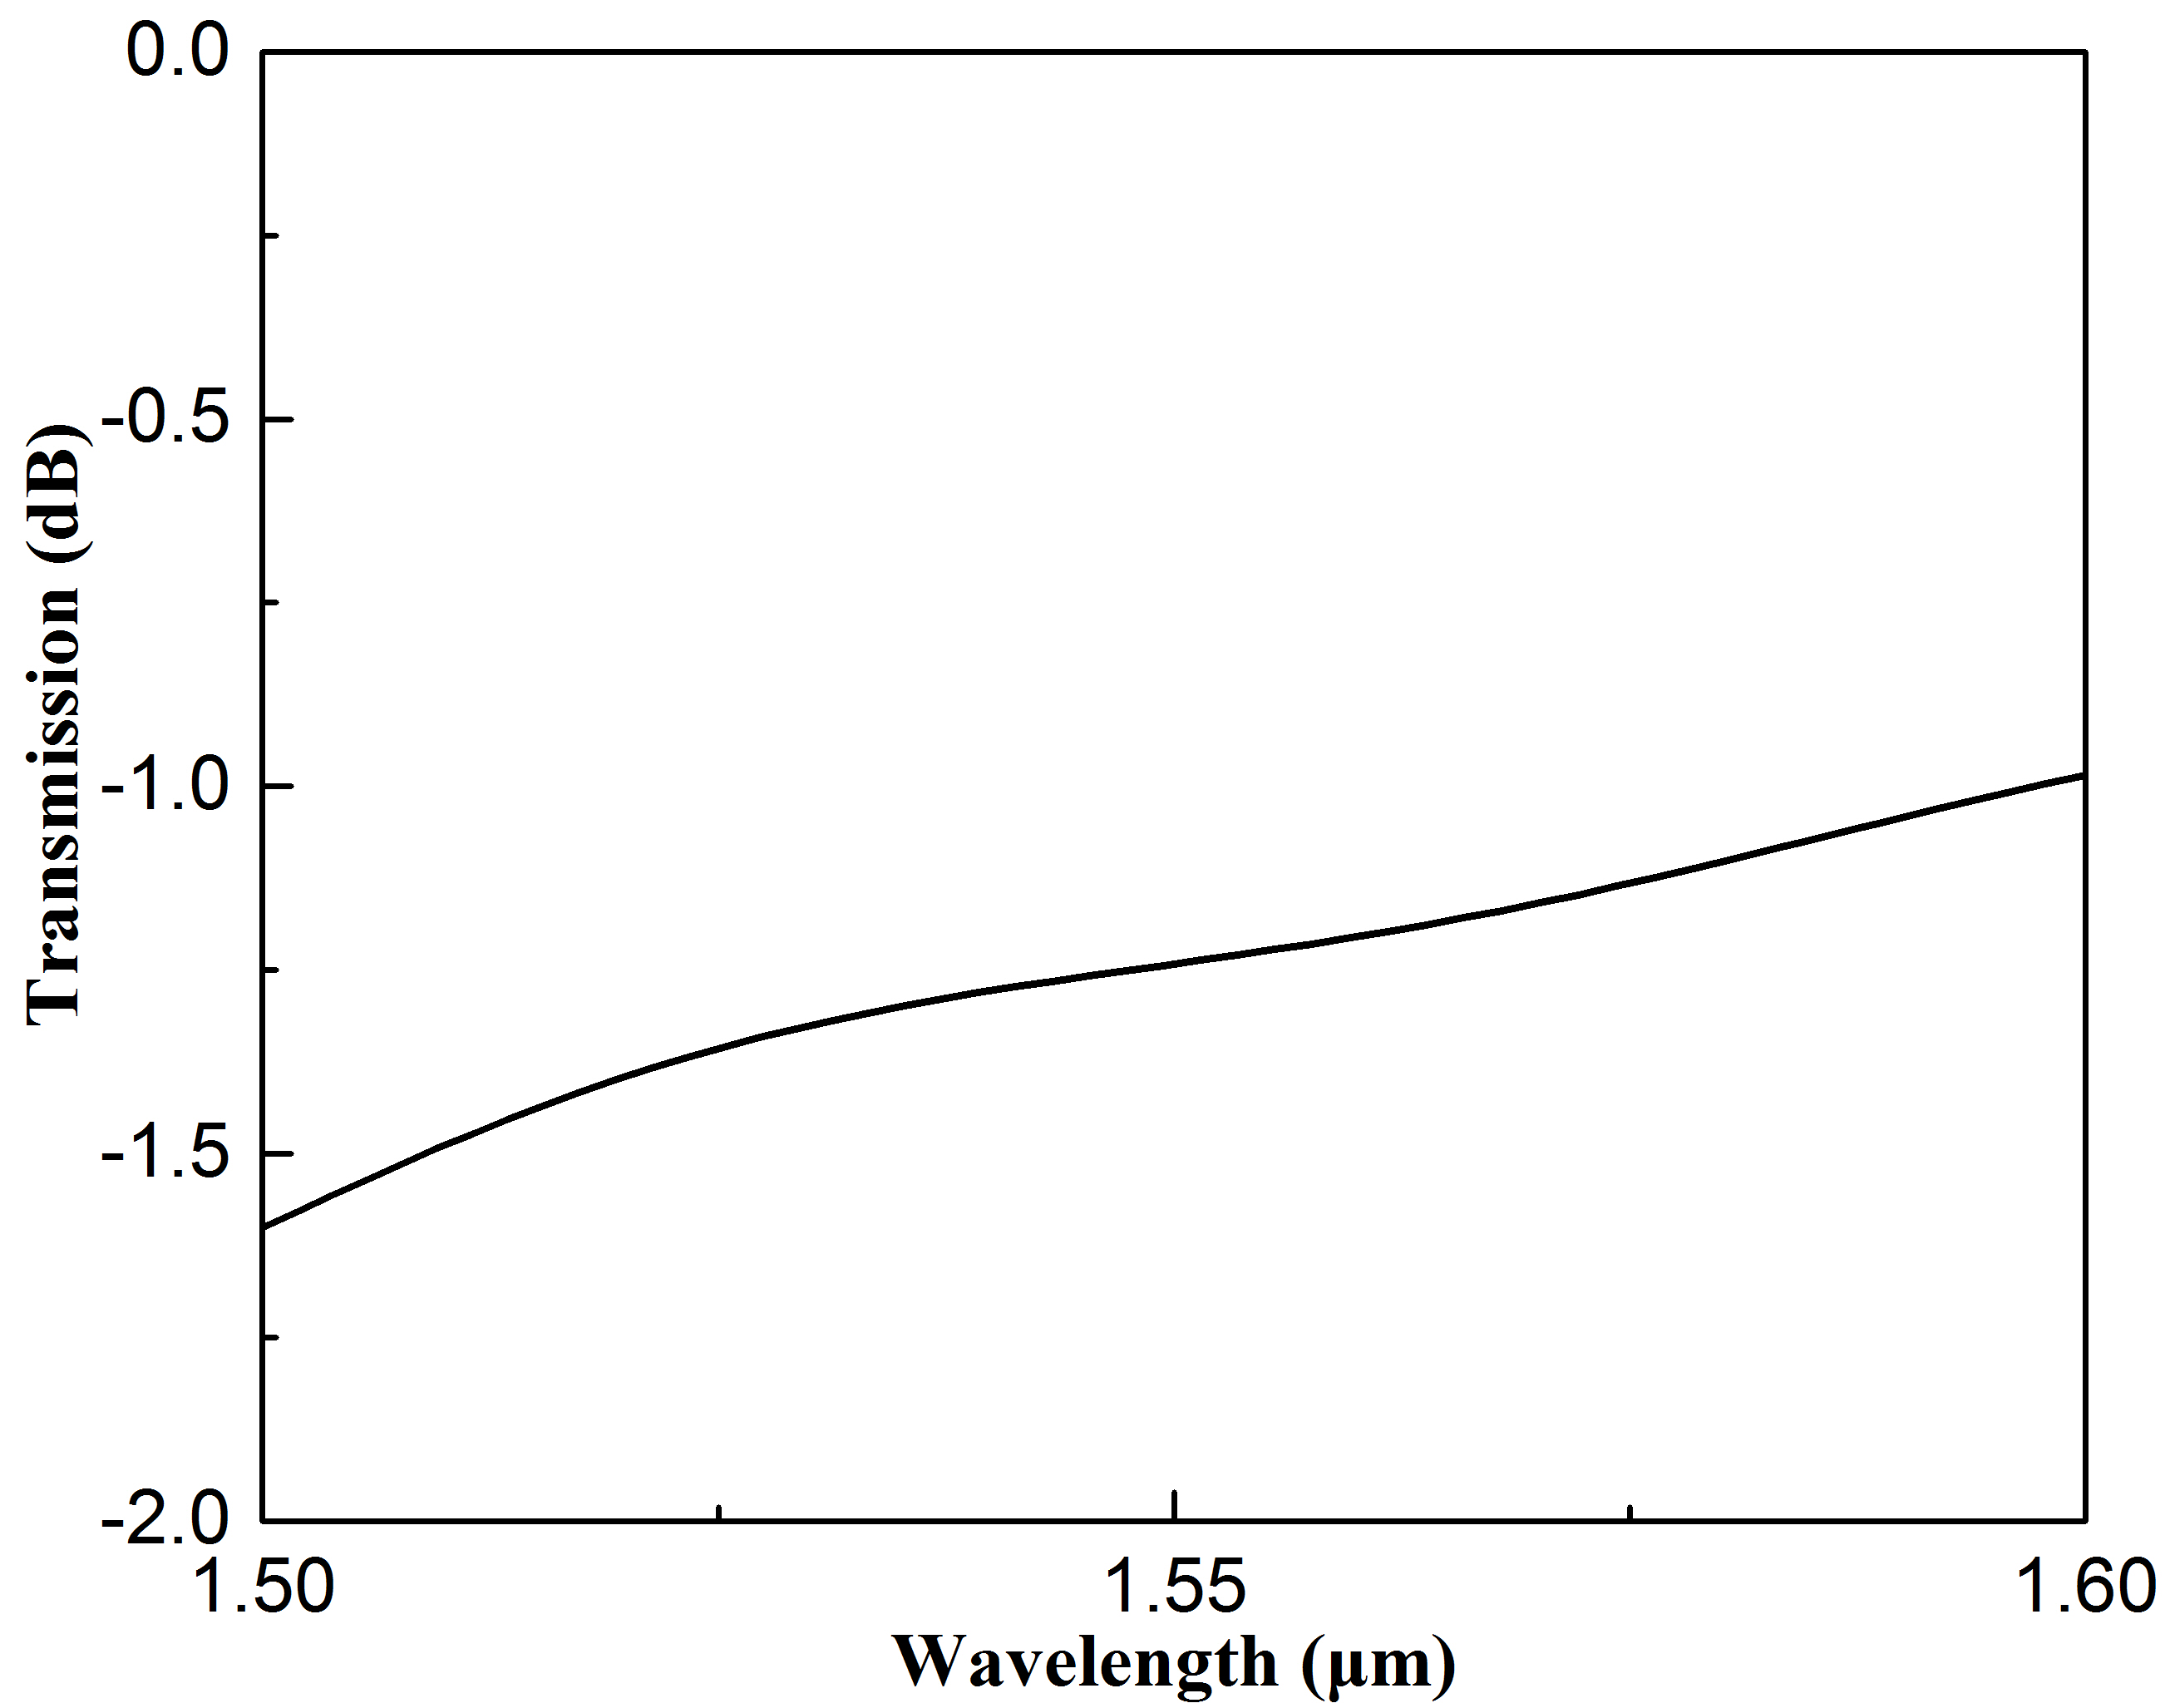
\includegraphics[width=12cm]{./Pictures/edg_dbr_loss.jpg}
	\captionsetup{justification=centering}
	\caption{DBR反射镜反射谱}
	\label{edg_dbr_loss}
\end{figure}

\begin{figure}[htb]
	\centering
	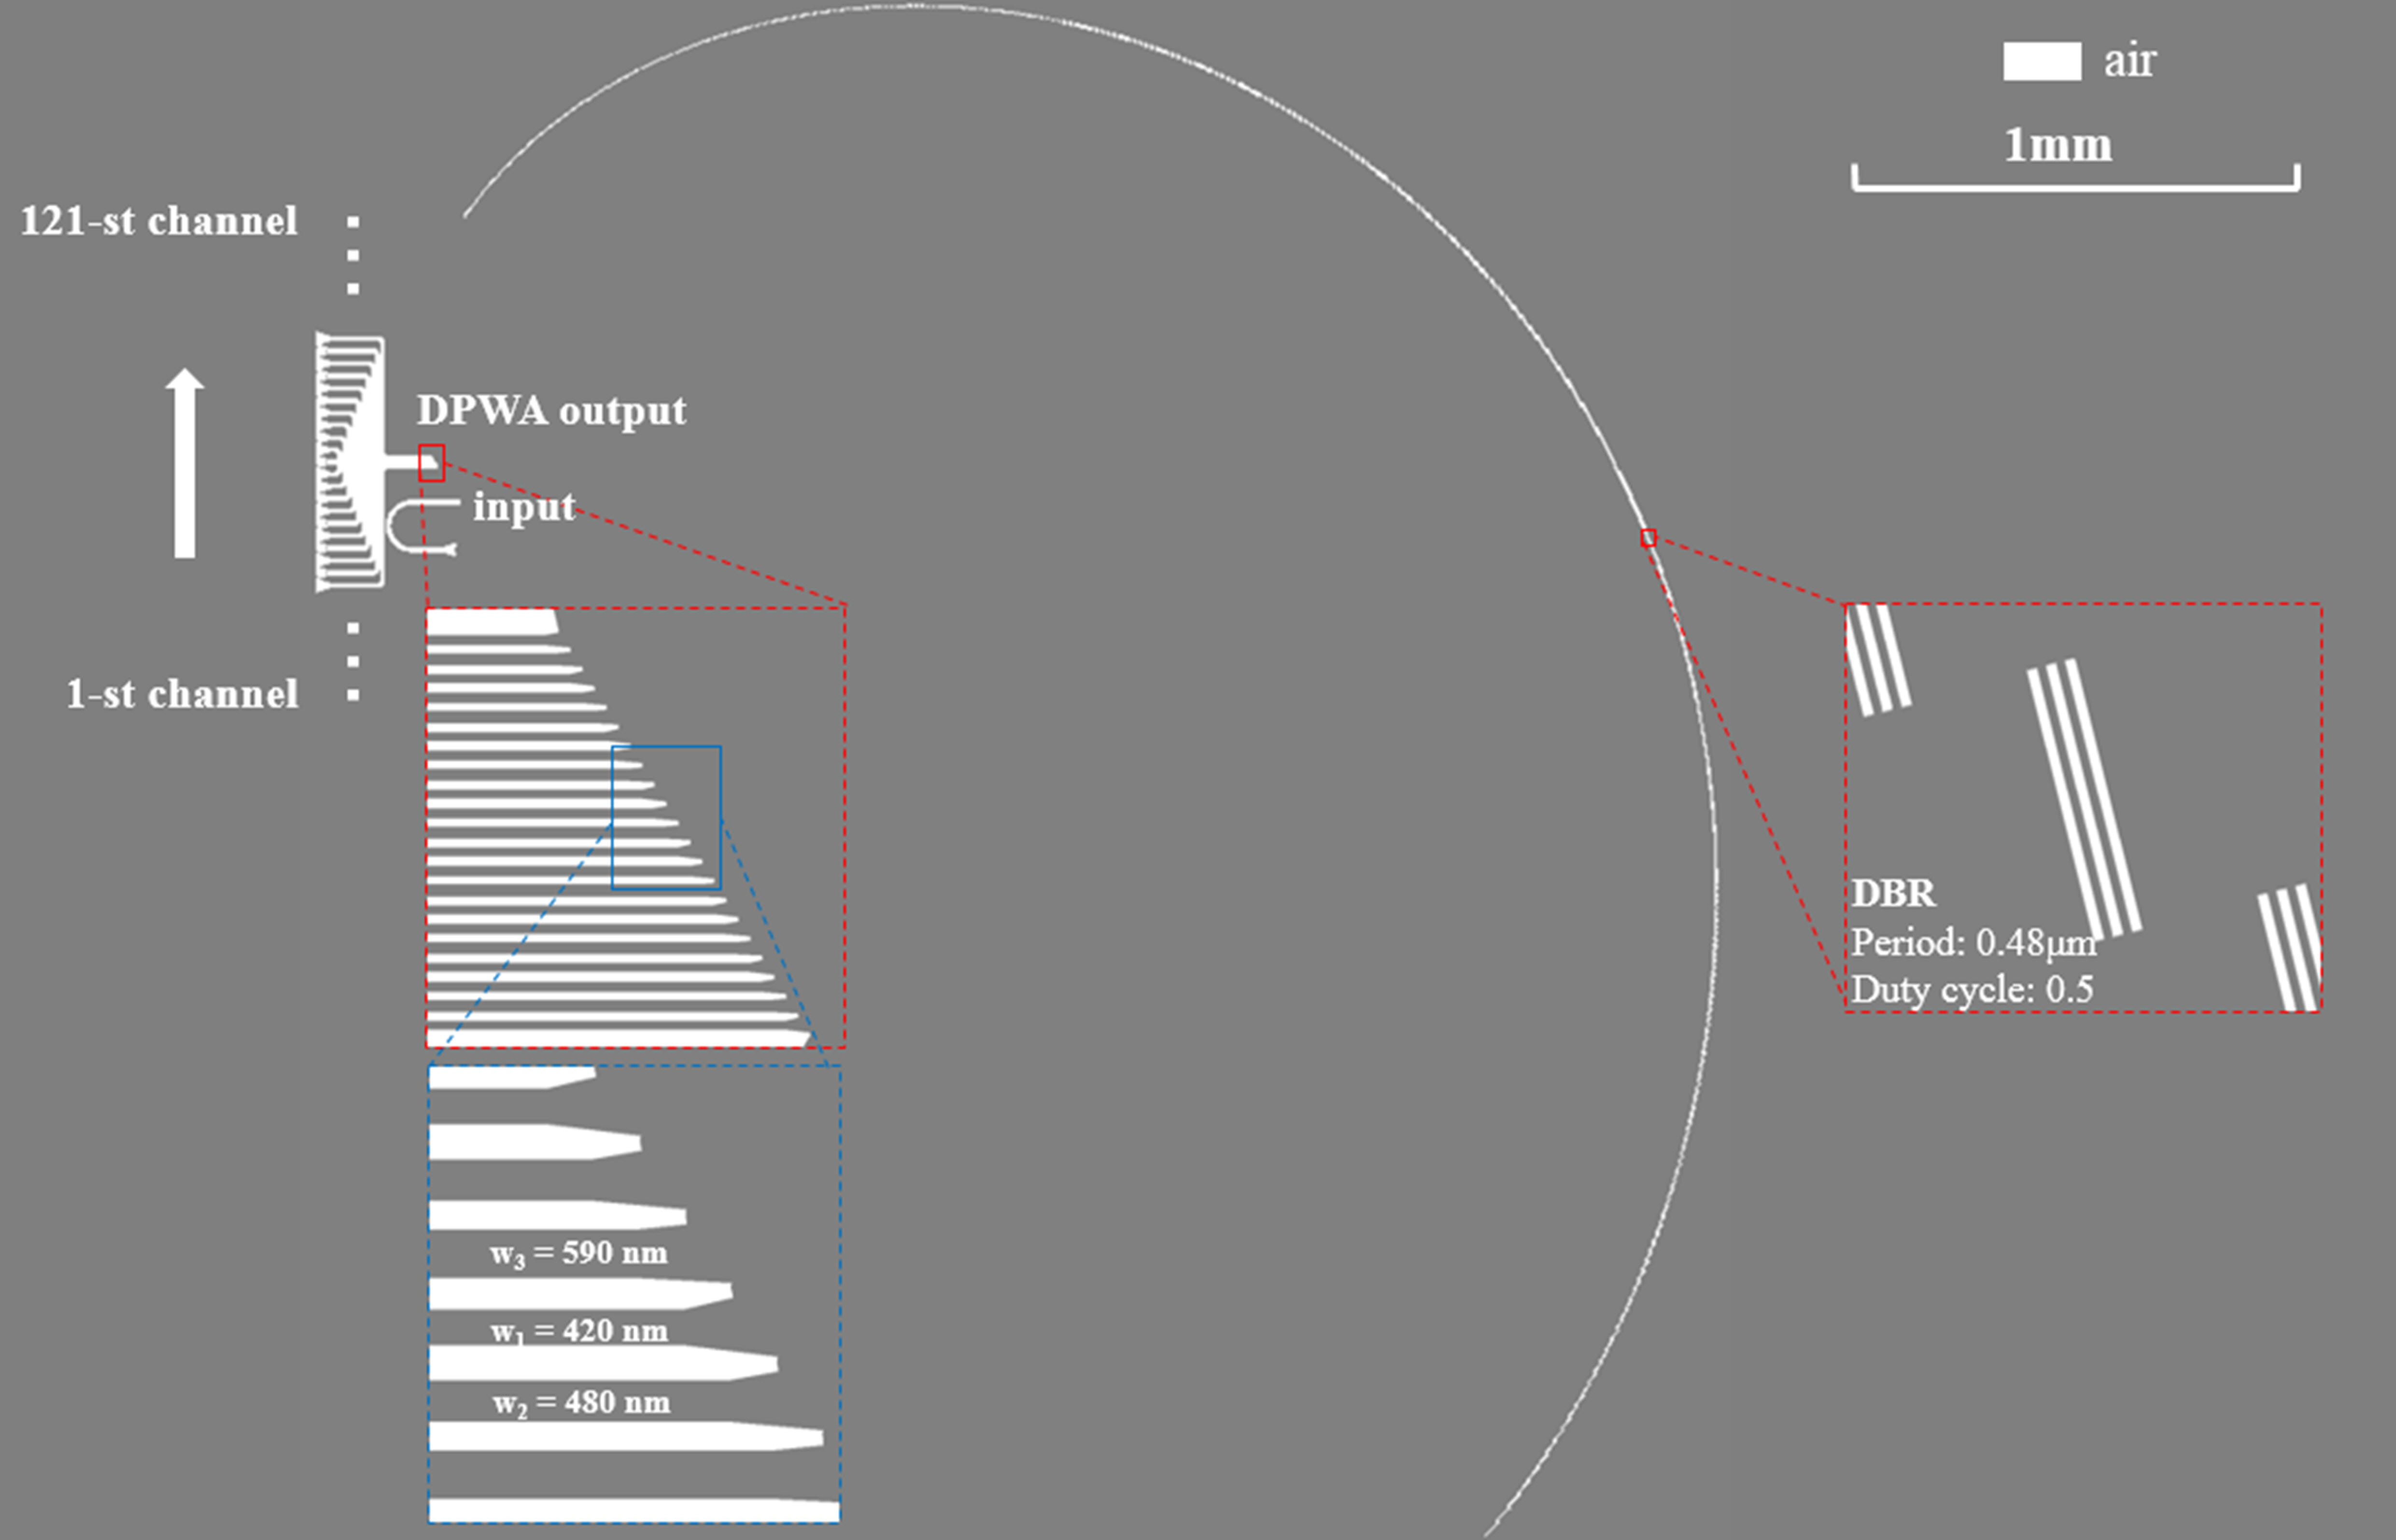
\includegraphics[width=16cm]{./Pictures/edg_layout.jpg}
	\captionsetup{justification=centering}
	\caption{EDG光谱仪的结构示意图}
	\label{edg_layout}
\end{figure}

我们将EDG光谱仪的参数选取如下:通道数设为121,通道间隔为0.5~$nm$,干涉级次为15,工作模式为TE模式,此时的自由光谱范围(free spectrum range, FSR)约为80~$nm$。由于通道数较多,我们使用了具有两个完美成像点的设计方法\cite{horst2009silicon,horst2008echelle},该方法可以减小串扰和通道的不均匀性。我们将两个完美成像点设置在第30和第90个通道(中间为第61通道),那么所有反射镜的坐标位置就可以由两组椭圆的交点来确定。第一组椭圆的两个焦点分别位于输入端口和第30个输出通道端口,第二组椭圆的两个焦点分别位于输入端口和第90个输出通道端口。输入波导与输出波导跟一般EDG放置在罗兰圆上不同,而是放置在一条直线上,输入波导与中心输出波导间距100~$\mu m$,输出波导采用上节设计的密集阵列波导。由于干涉级次选定之后,输入波导和输出波导到相邻两个反射镜的光程差即被确定,通过不断改变两个椭圆的长轴长度,长度差即为干涉级次所确定的光程差,就可以得到一些列的交点,这些交点就是反射镜的中心点位置,反射光栅的角度由闪耀条件所确定。由于干涉级次决定的是光程差,但此时输入波导经第一个反射镜到输出波导的光程绝对值并不确定,我们可以扫描绝对光程,使得边缘通道的相差达到最小,尽量提升边缘通道的性能。最终,该EDG光谱仪的结构如图\ref{edg_layout}所示,反射镜一共有620个。光从输入波导进入自由传输区(FPR),经DBR反射镜反射并重新聚焦到输出波导,由于不同波长的光所经历的光程不一样,所以他们的干涉增强点位置不同,从而实现不同波长的光的分离。该器件的总尺寸为3~$mm~\times$~3~$mm$。图中的通道数只有21,而不是设计的121,是考虑到用我们实验室的电子束曝光机(Raith 150$^{TWO}$)加工的可行性,虽然EBL的加工精度相比光刻会高很多,但是曝光时间却需要很长。用EBL来制作我们设计的EDG光谱仪,曝光的时间随着通道数目的增多呈指数关系增长。因为随着通道数增多,每根波导的长度都需要增加以避免与输入波导的交叉。通过实验,我们发现加工21通道的该EDG光谱仪需要大概90分钟,41通道的需要大概250分钟,61通道的加工时间已经到了大概480分钟,长时间的曝光,EBL会产生较大的拼接错位问题,从而导致器件的性能受到影响。如果将该EDG光谱仪委托有能力的半导体公司进行流片,这个问题就可以得到解决,而且器件的尺寸并不会因为通道数变多增加太多,因为该EDG光谱仪的大小主要由反射面的尺寸所决定。


我们用标量衍射法\cite{pathak2014silicon}对EDG光谱仪进行了仿真,如图\ref{edg_diffraction_method}所示,在$x_{0}$轴处的光场$U(x_{0})$可以用公式\ref{diffraction_method}计算得到距离$x_{0}$轴为z的$x_{1}$轴处光场$U(x_{1})$:

\begin{figure}[htb]
	\centering
	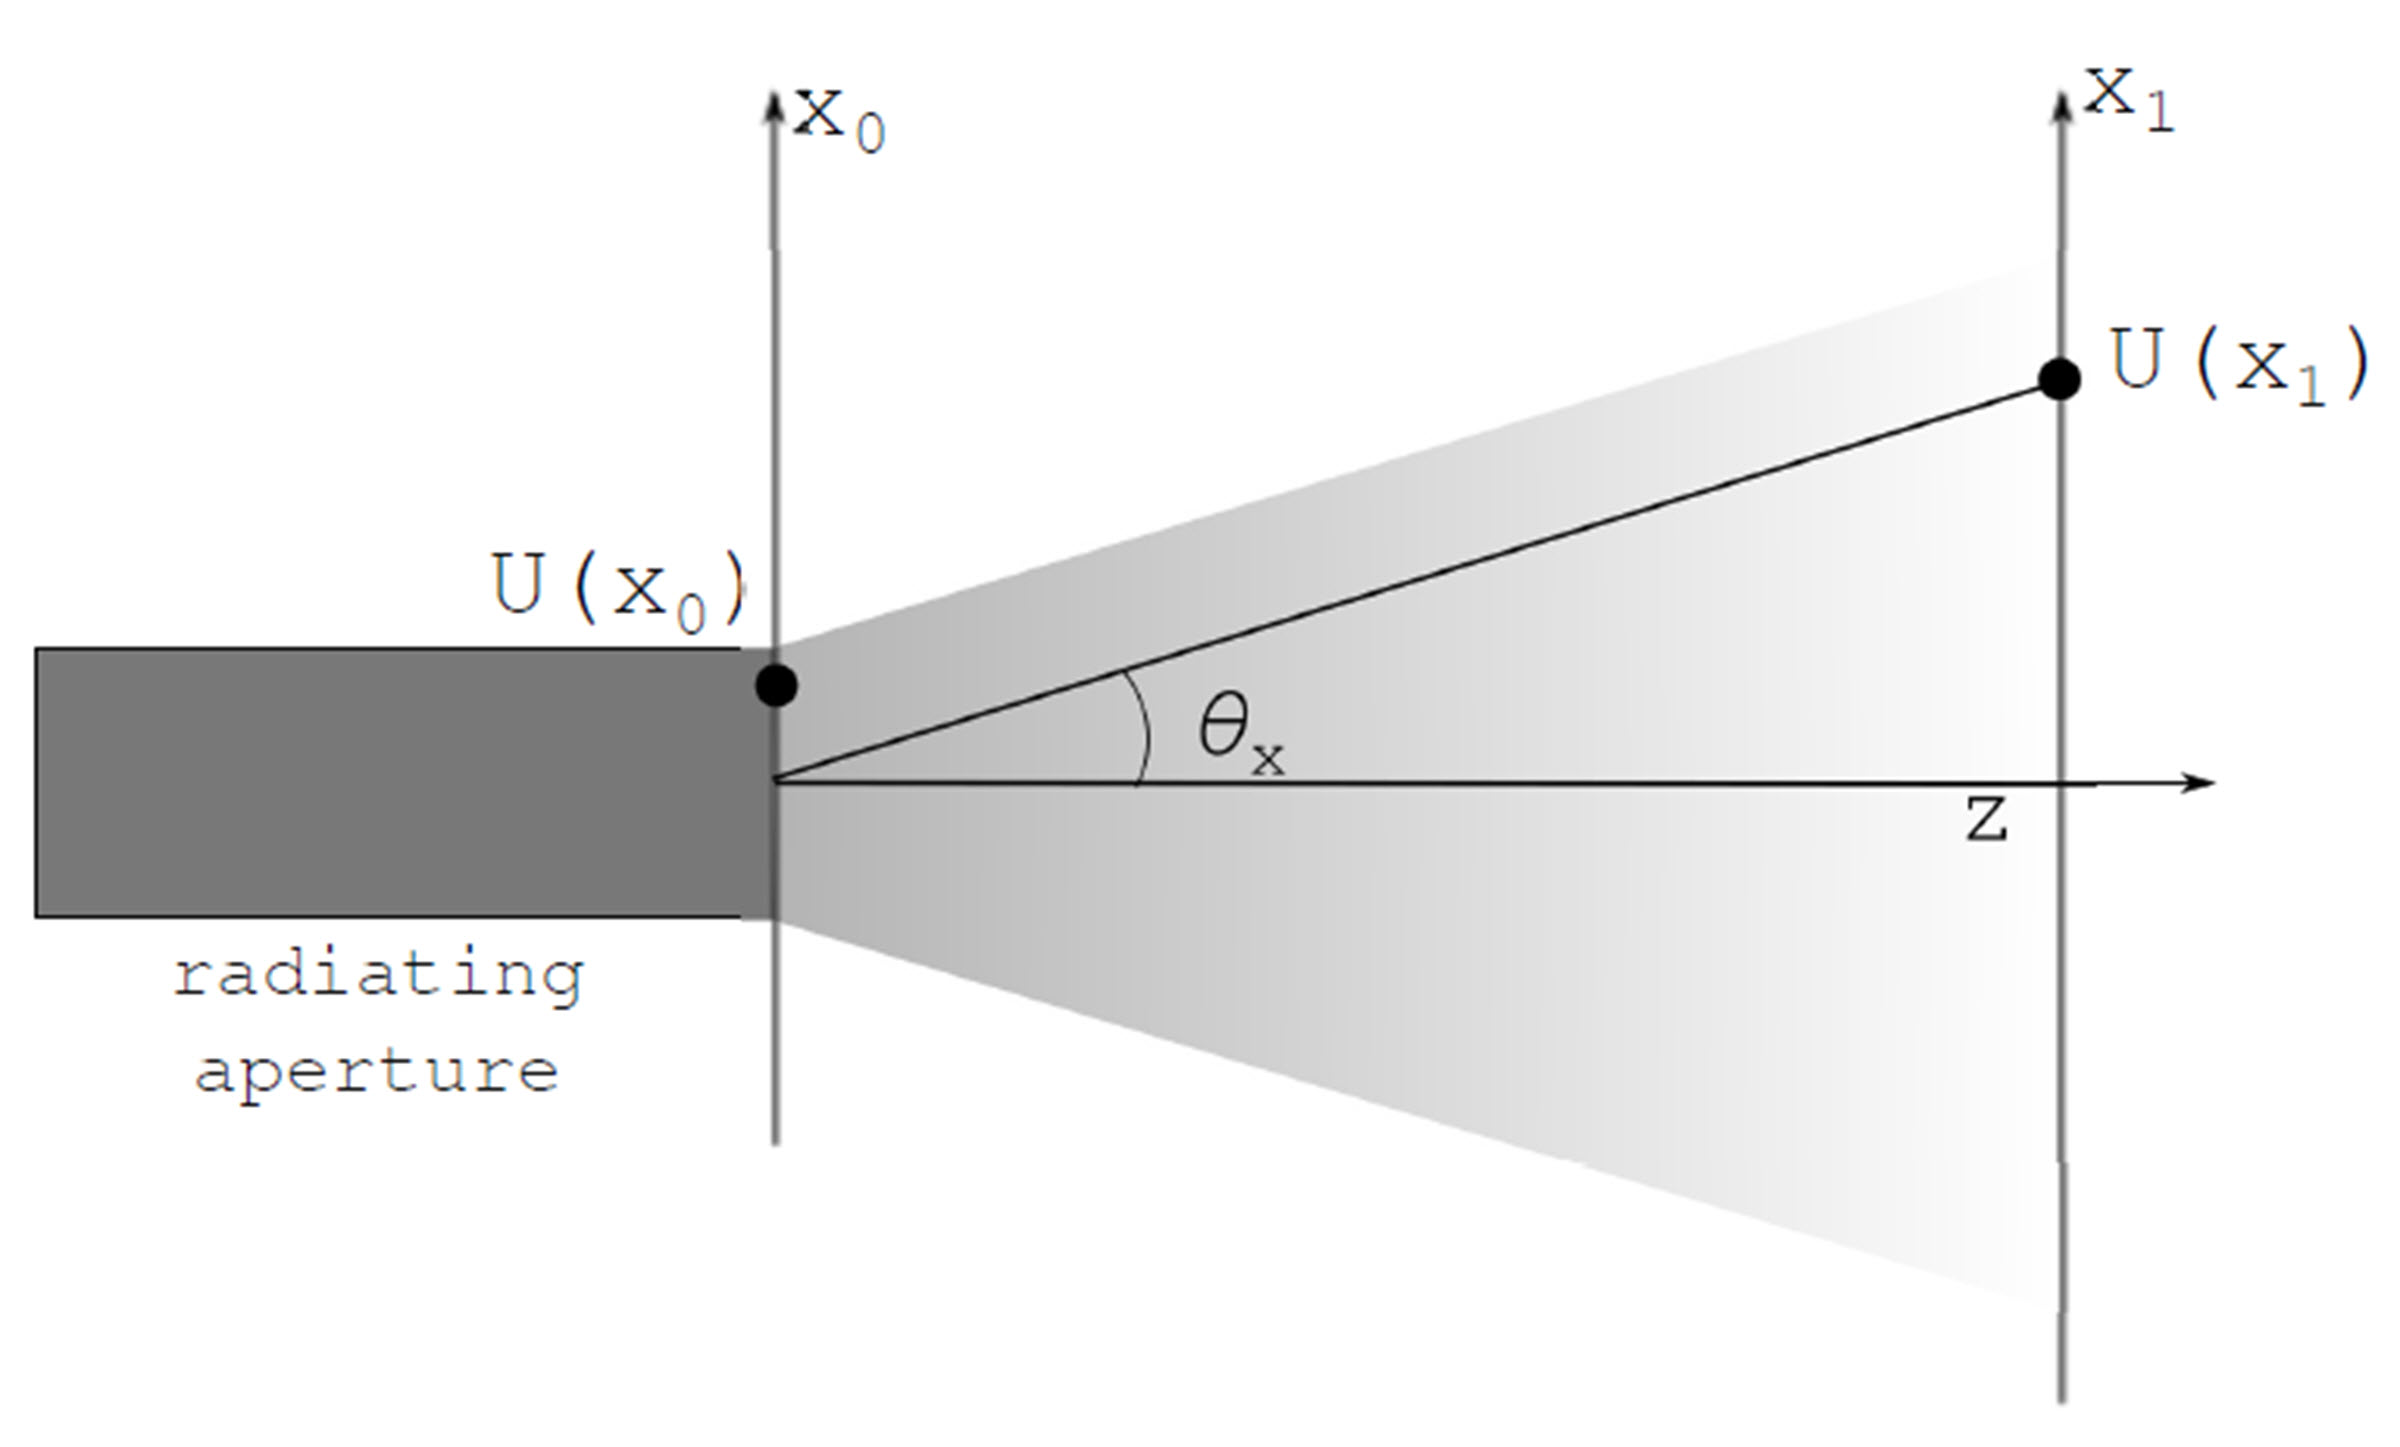
\includegraphics[width=13cm]{./Pictures/edg_diffraction_method.jpg}
	\captionsetup{justification=centering}
	\caption{标量衍射法坐标图}
	\label{edg_diffraction_method}
\end{figure}

\begin{equation}
\label{diffraction_method}
U(x_{1})=\dfrac{je^{-jkz}e^{-jkx_{0}^2/2 z}}{\lambda z}\int_{-\infty}^{\infty}U(x_{0})e^{-jkx_{0}^{2}/2z}e^{-j2\pi x_{1}x_{0}/\lambda z}\,dx_{0}
\end{equation}

当z距离很大时($z>>k(x_{0}^{2})_{max}/2$),公式\ref{diffraction_method}可以简化成公式\ref{diffraction_method_simplified}:

\begin{equation}
\label{diffraction_method_simplified}
U(x_{1})=\dfrac{je^{-jkz}e^{-jkx_{0}^2/2 z}}{\lambda z}\int_{-\infty}^{\infty}U(x_{0})e^{-j2\pi x_{1}x_{0}/\lambda z}\,dx_{0}
\end{equation}

公式中,$j$是虚数单位,$k$是波矢。从公式\ref{diffraction_method_simplified}中我们可以看出如果将空间频率定义为$f_{x}=-x_{1}/\lambda z$,则$x_{1}$轴处的场$U(x_{1})$是$x_{0}$轴处场$U(x_{0})$的傅里叶变换,该区域通常被叫做远场或者也可以叫做弗朗和费衍射区。

\begin{figure}[htb]
	\centering
	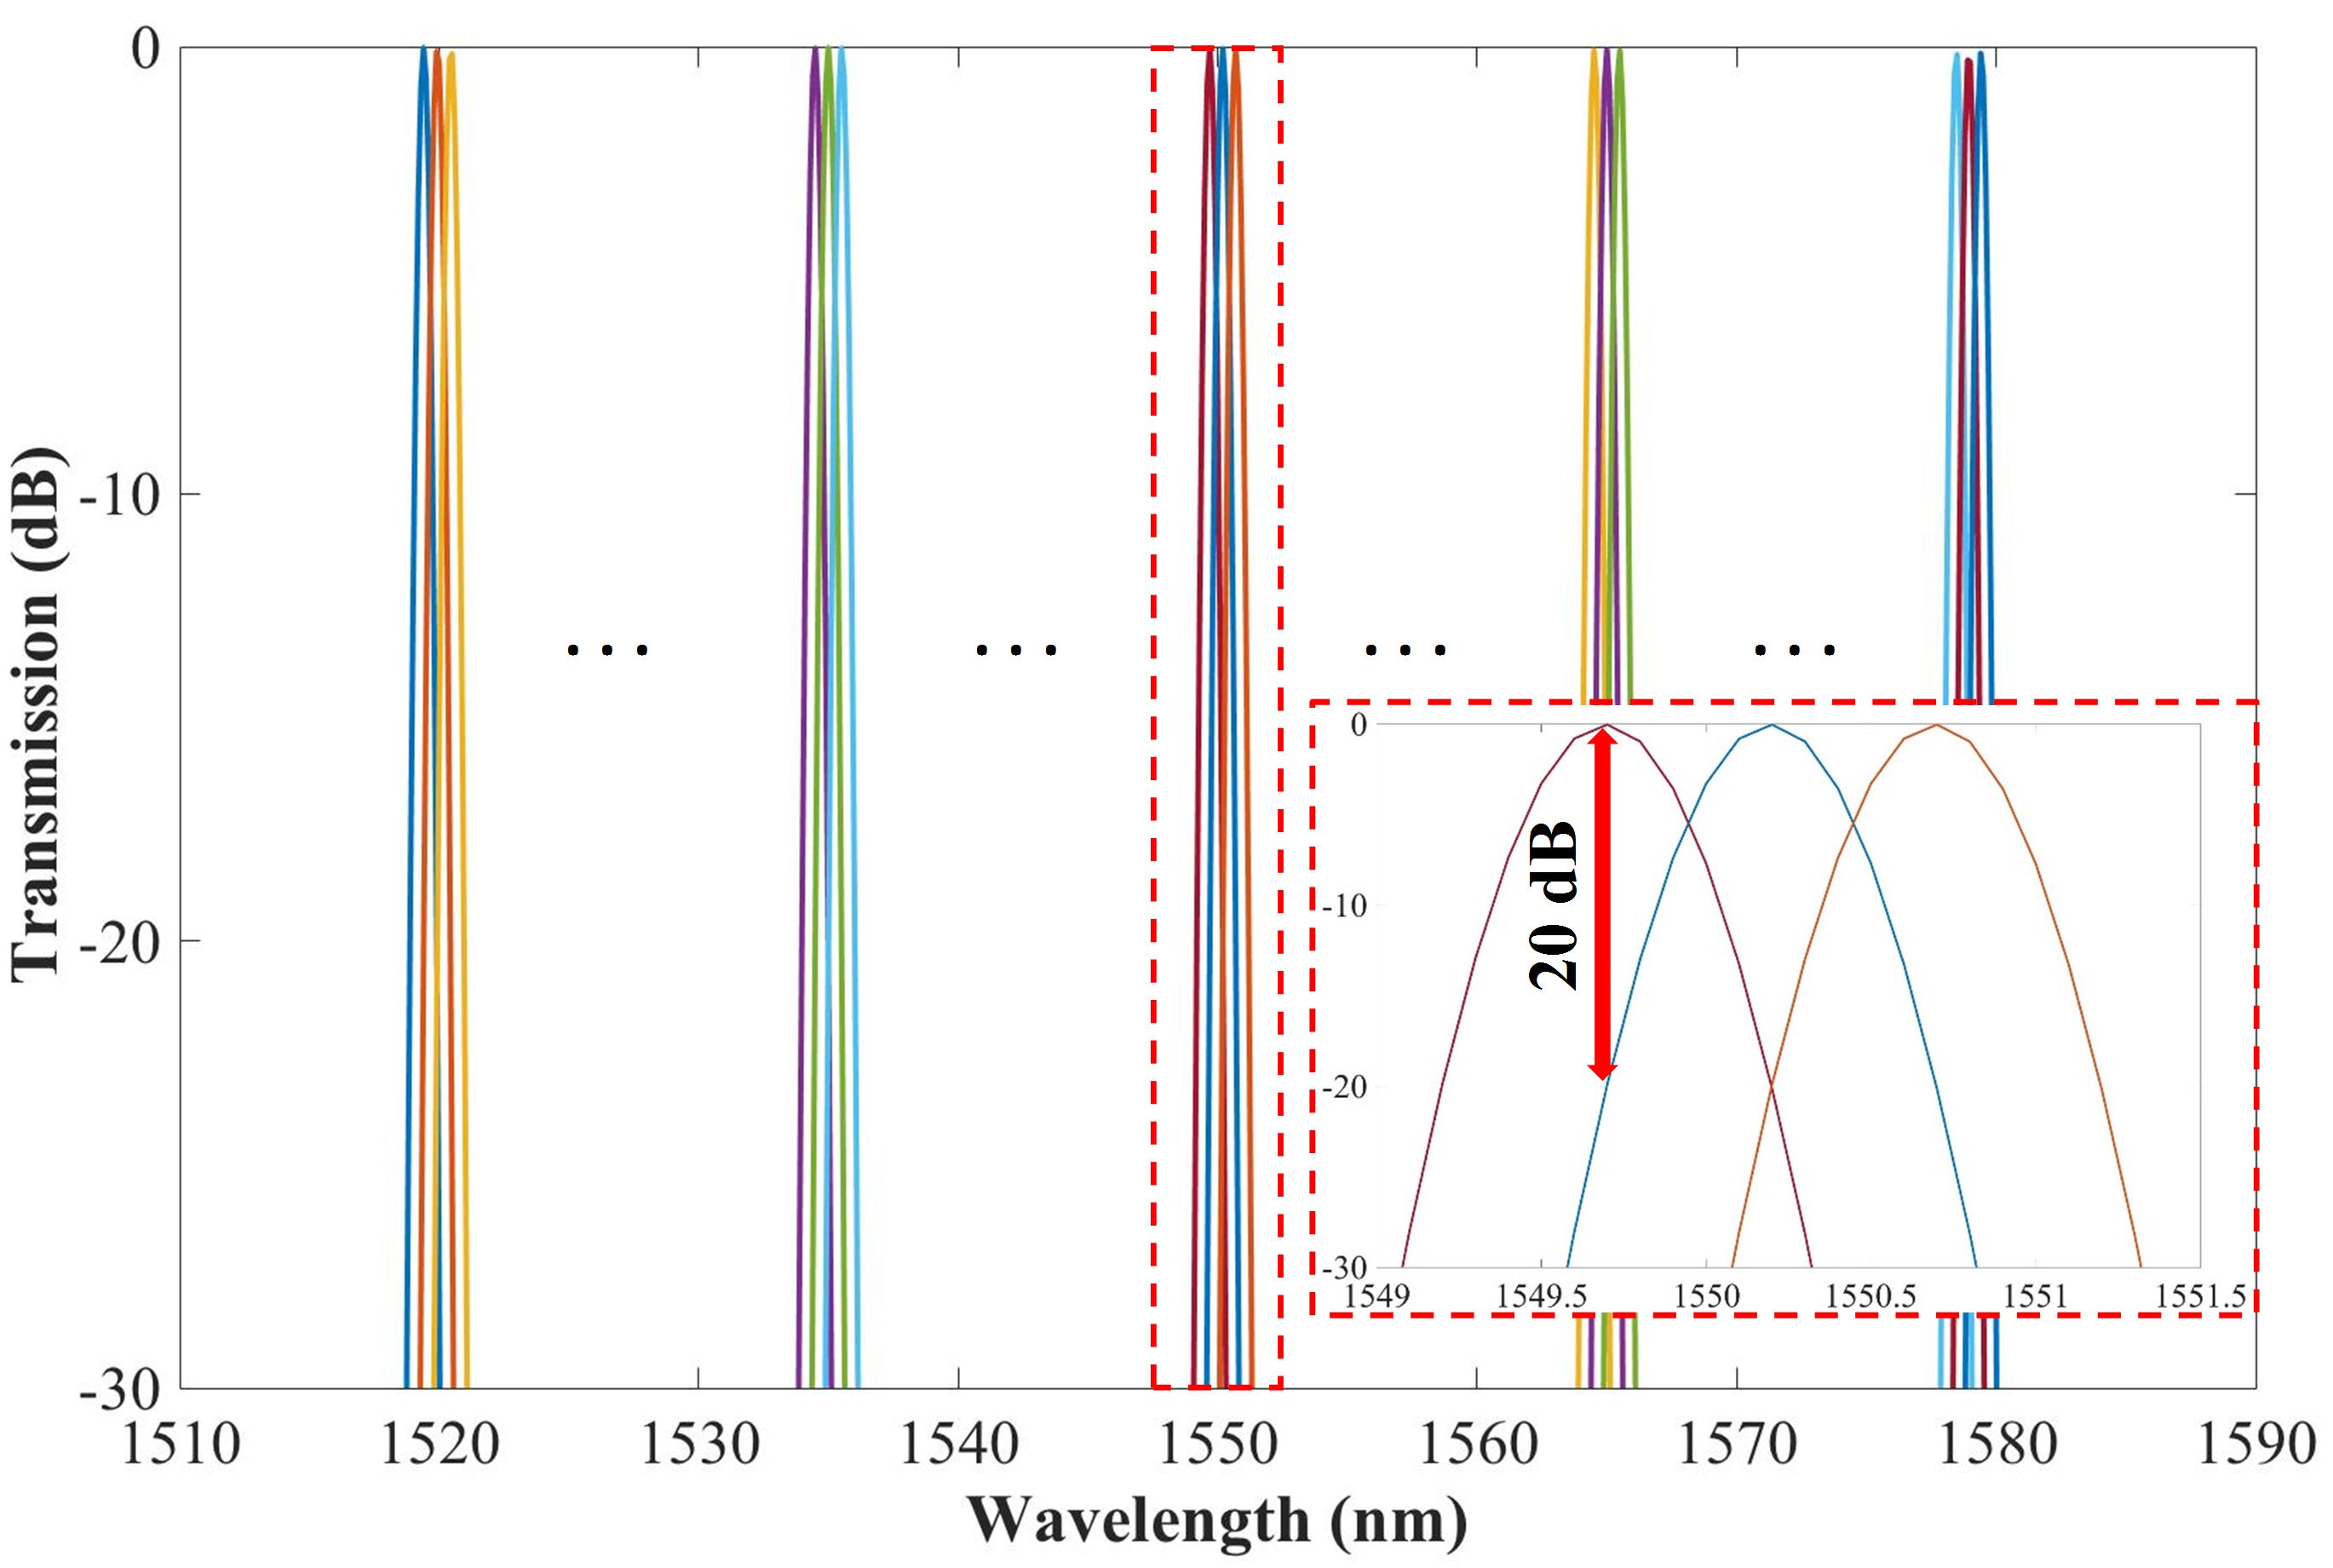
\includegraphics[width=14cm]{./Pictures/edg_simulated_spectrum.jpg}
	\captionsetup{justification=centering}
	\caption{EDG光谱仪仿真谱线}
	\label{edg_simulated_spectrum}
\end{figure}

该EDG光谱仪的仿真结果如图\ref{edg_simulated_spectrum}所示,为了方便,仿真时将DBR反射镜的反射率设为100\%。由于通道数目较多,图中仅显示了中心附近通道,完美成像点处附近通道以及边缘通道的响应谱线。仿真结果显示,中心通道为1550~$nm$,通道间隔为0.5~$nm$,3~dB带宽为0.3~$nm$,通道之间串扰为-20~dB,通道不均匀性小于0.2~dB,表明基于两个完美成像点的设计方法设计的EDG光谱仪可以实现很好的多通道性能。

\section{硅基EDG光谱仪的工艺制作}
\subsection{工艺步骤}
该EDG光谱仪工艺制作是基于SOI平台上完成的,其中硅层厚度为220 $nm$,二氧化硅绝缘层厚度为2~$\mu m$。EDG光谱仪的制作过程如图\ref{edg_fabrication}所示。

\begin{figure}[htb]
	\centering
	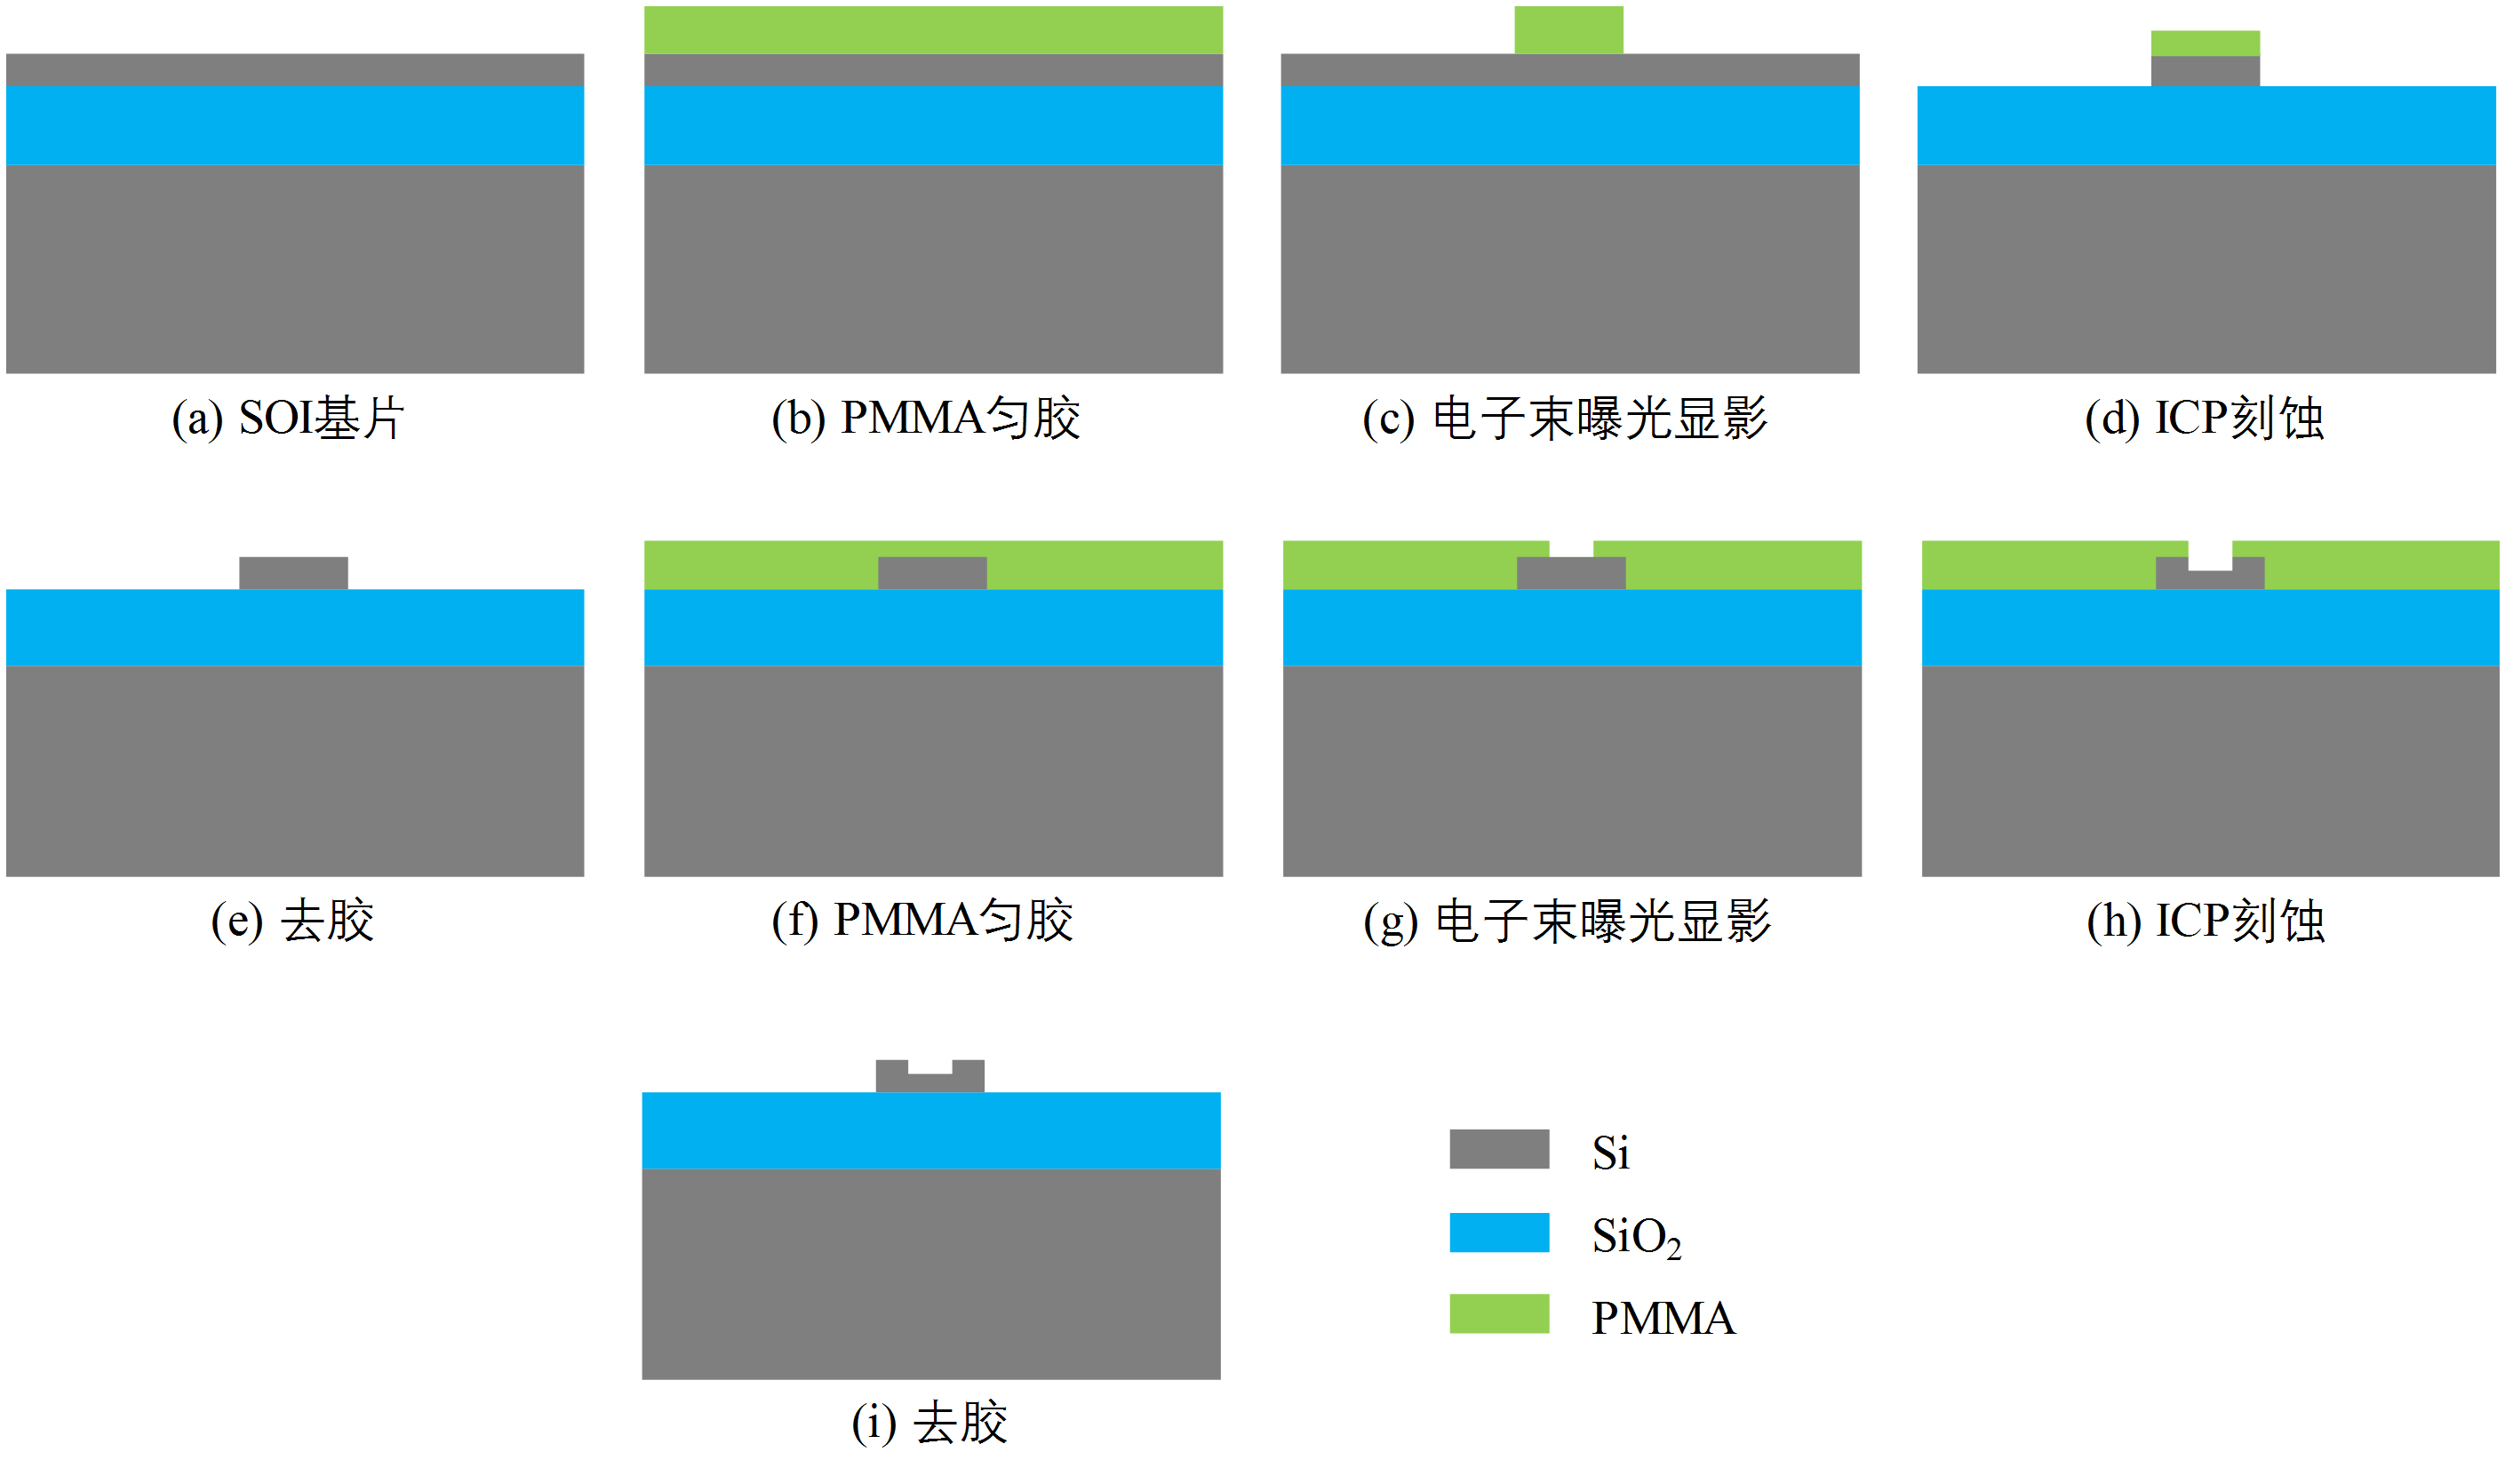
\includegraphics[width=15cm]{./Pictures/edg_fabrication.jpg}
	\captionsetup{justification=centering}
	\caption{硅基EDG光谱仪的制作主要工艺流程图}
	\label{edg_fabrication}
\end{figure}

\begin{enumerate}[(a)]
	\item
	用解理刀和解理钳解理一块适当大小的SOI芯片,用丙酮、甲醇、异丙醇各超声5分钟,去除表面的有机物。然后准备浓H\SB{2}SO\SB{4}:H\SB{2}O\SB{2}=1:1(体积比)的食人鱼溶液,浸泡2\~{}3小时,之后用BOE(buffered oxide etch)腐蚀液浸泡几秒钟,去除基片表面的氧化层,使其由亲水表面变成疏水表面,易于旋涂光刻胶。之后,然后放于180~$^{\circ}$C热板上烘烤15~$min$,去除水汽,不然会在匀胶的时候会匀不上。
	\item 
	使用匀胶机在SOI芯片表面旋涂一层厚度约为270 $nm$的正性电子束光刻胶PMMA 950K 679.04,其匀胶参数为前转2000~rpm~3~$s$,后转4000~rpm~59~$s$。然后将匀好胶的芯片放到180~$^{\circ}$C的热板上前烘10~$min$。
	\item
	用EBL将设计好的掩模在匀好胶的芯片上曝光,将掩模图案转移到胶上形成潜影,曝光过程中的加速电压为20 kV,电子束光阑孔径为10~$\mu m$,曝光基准剂量为200~$\mu C/cm^{2}$,剂量因子是1.4。曝光完成后,用MIBK(methyl isobutyl ketone) : IPA(isopropyl alcohol)~=~1:3(体积比)混合溶液显影35~$s$,再置于IPA中定影40~$s$,然后用去离子水冲洗30~$s$,用氮气枪将芯片吹干,用热板60~$^{\circ}$C烘烤5~$min$,再将热板温度设升到到90~$^{\circ}$C并保持,继续烘烤几分钟,保证总的坚膜时间为15~$min$,提高胶的抗刻蚀性。
	\item
	使用ICP刻蚀硅层,将胶上的图形转移到硅层上,刻蚀使用的气体为SF\SB{6}和C\SB{4}F\SB{8},刻蚀深度为220~$nm$,形成深刻蚀的波导与DBR反射镜。
	\item 
	将刻蚀之后的芯片放入丙酮,在摇床上摇10~$min$去除残胶。之后用去离子水冲洗,用热板180~$^{\circ}$C烘烤15~$min$,去除水汽。
	\item 
	匀PMMA胶,同(b)。
	\item 
	曝光显影,同(c),但是曝光参数变为加速电压为30~kV,电子束光阑孔径为20 $\mu m$,曝光基准剂量为300~$\mu C/cm^{2}$,剂量因子为1.4。
	\item 
	使用ICP刻蚀,由于我们设计的EDG工作在TE偏振模式下,我们的TE光栅采用的是浅刻蚀设计,故这一步刻蚀深度为70~$nm$。
	\item 
	将刻蚀之后的芯片放入丙酮,在摇床上摇10~$min$去除残胶,再放入食人鱼溶液浸泡2\~{}3小时,最后用氧气等离子体清洗30~$min$,确保将所有残胶去除干净,以免影响测试结果。
\end{enumerate}
\subsection{EBL描边法}

\begin{figure}[htb]
	\centering
	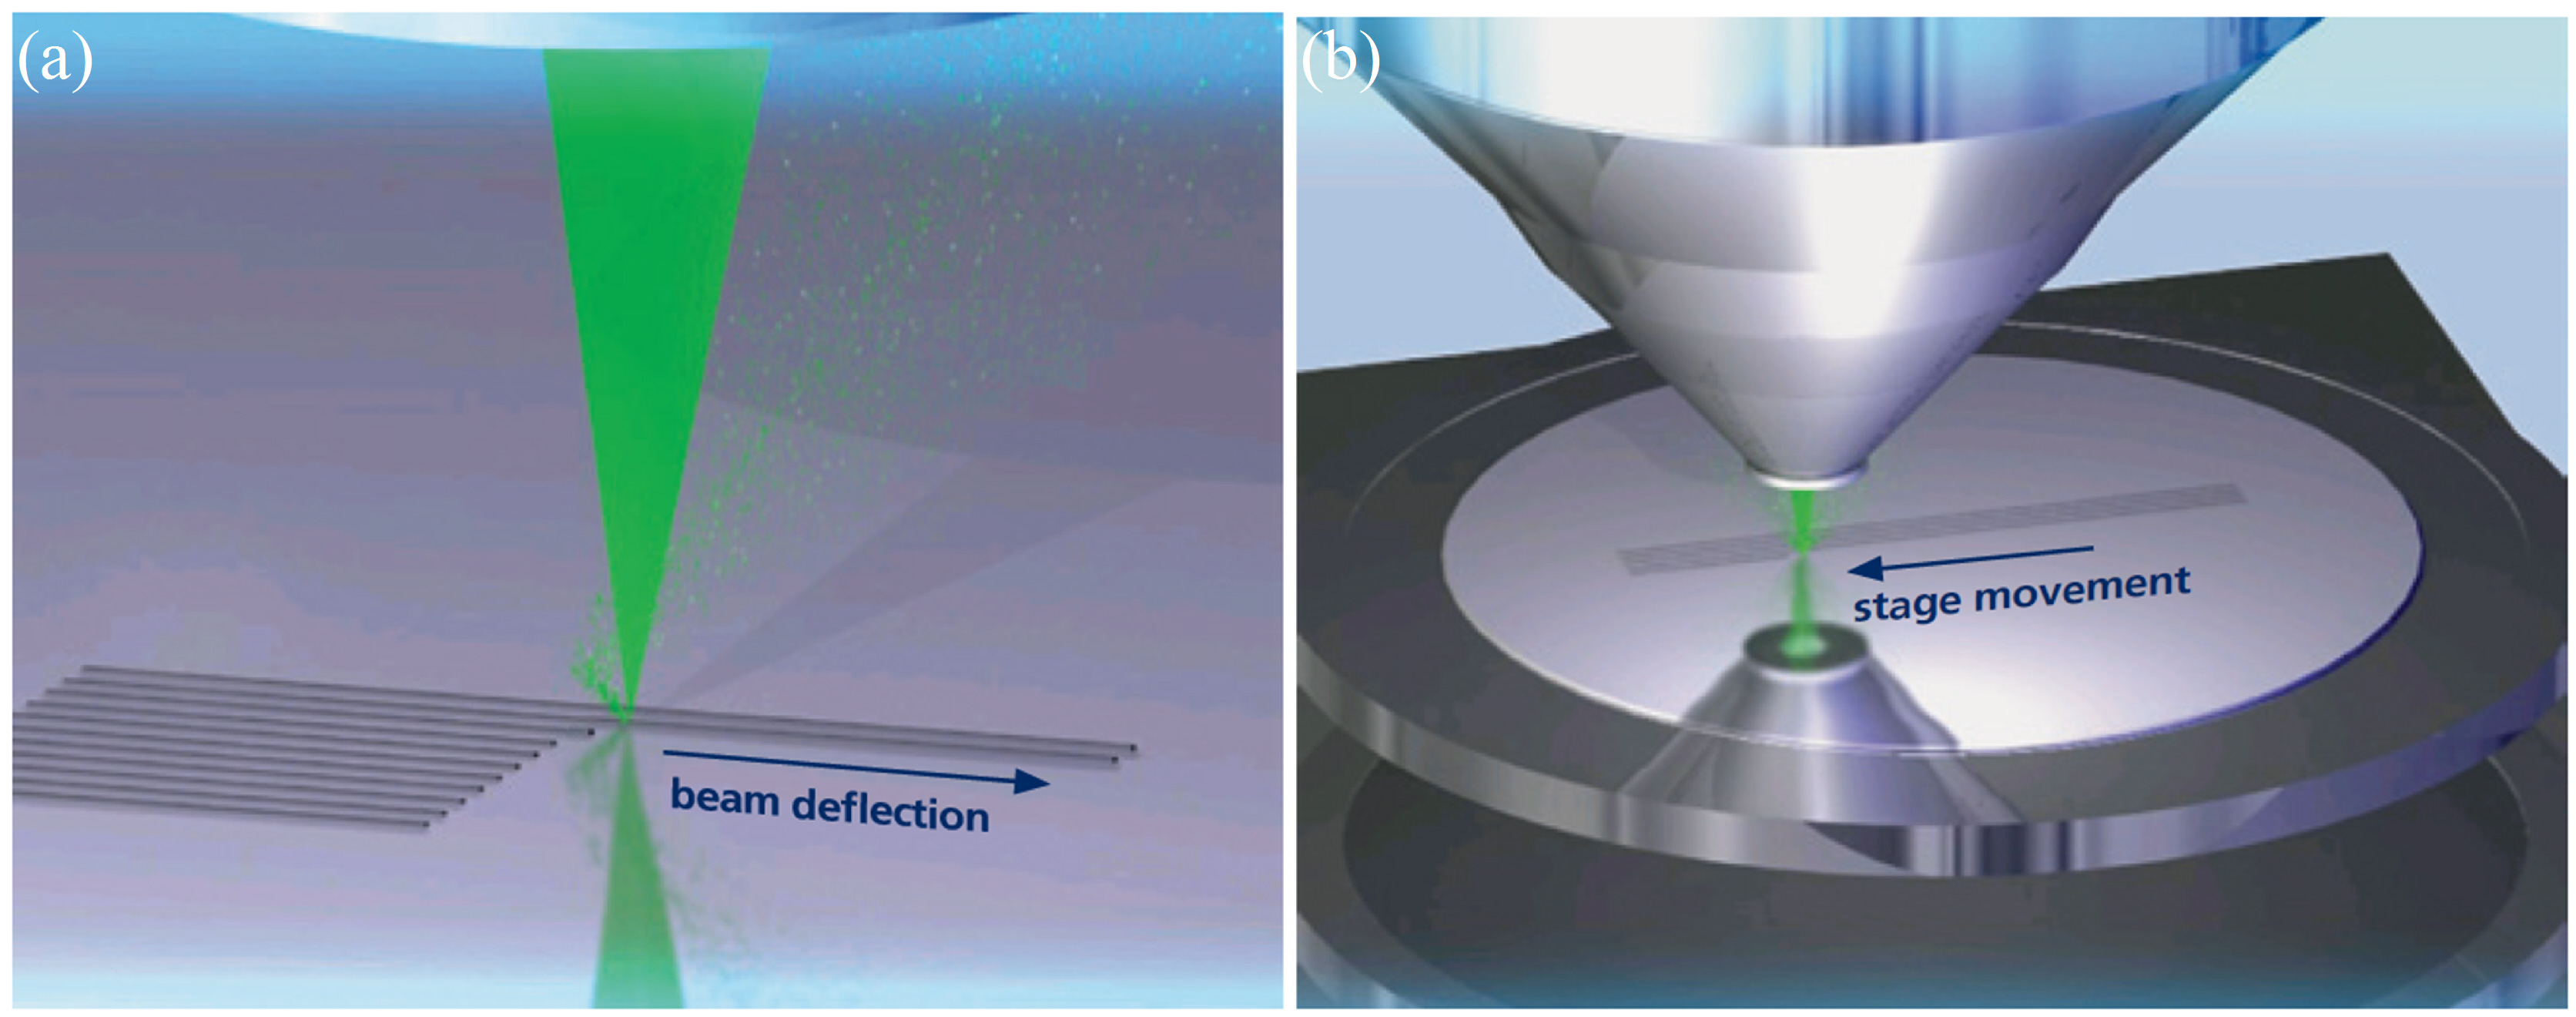
\includegraphics[width=15cm]{./Pictures/edg_pattern_mode.jpg}
	\captionsetup{justification=centering}
	\caption{EBL的两种工作模式,(a)拼接模式;(b)连续模式\cite{piaszenskicontinuous}}
	\label{edg_pattern_mode}
\end{figure}

首先分别介绍我们的EBL RAITH 150\SP{TWO}的两种工作模式:拼接模式和连续模式\cite{piaszenskicontinuous}。

拼接模式如图\ref{edg_pattern_mode}(a)所示,EBL将要曝光的图形分成一块块写场(writing field),一般都是100 $\mu m~\times$ 100~$\mu m $,然后按顺序依次用电子束曝光,曝光的时候载物台静止不动,电子束在不同的偏压控制下偏转完成该写场的曝光,然后移动载物台到下一个写场,直到完成所有区域的曝光。这种模式会有写场之间的拼接错位问题,当写场数量较少的时候,错位一般在几个$nm$量级,对器件影响有限,但当写场的数量很多时,错位会积累到较大的程度从而导致器件的性能受到影响。由于我们的EDG光谱仪总的曝光时间比较长,加工过程中电子枪的定位会出现漂移,加剧了拼接错位的问题。如果用拼接模式直接加工我们的EDG光谱仪,结果如图\ref{edg_misalignment}(a)所示,可以看到弯曲波导与直波导连接处出现了严重的错位问题,虽然经过曝光剂量,图形错位等的补偿之后,制作结果如图\ref{edg_misalignment}(b)所示,但是问题依然存在,这些制作的缺陷会导致光谱仪的插损与串扰性能都较差。

\begin{figure}[htb]
	\centering
	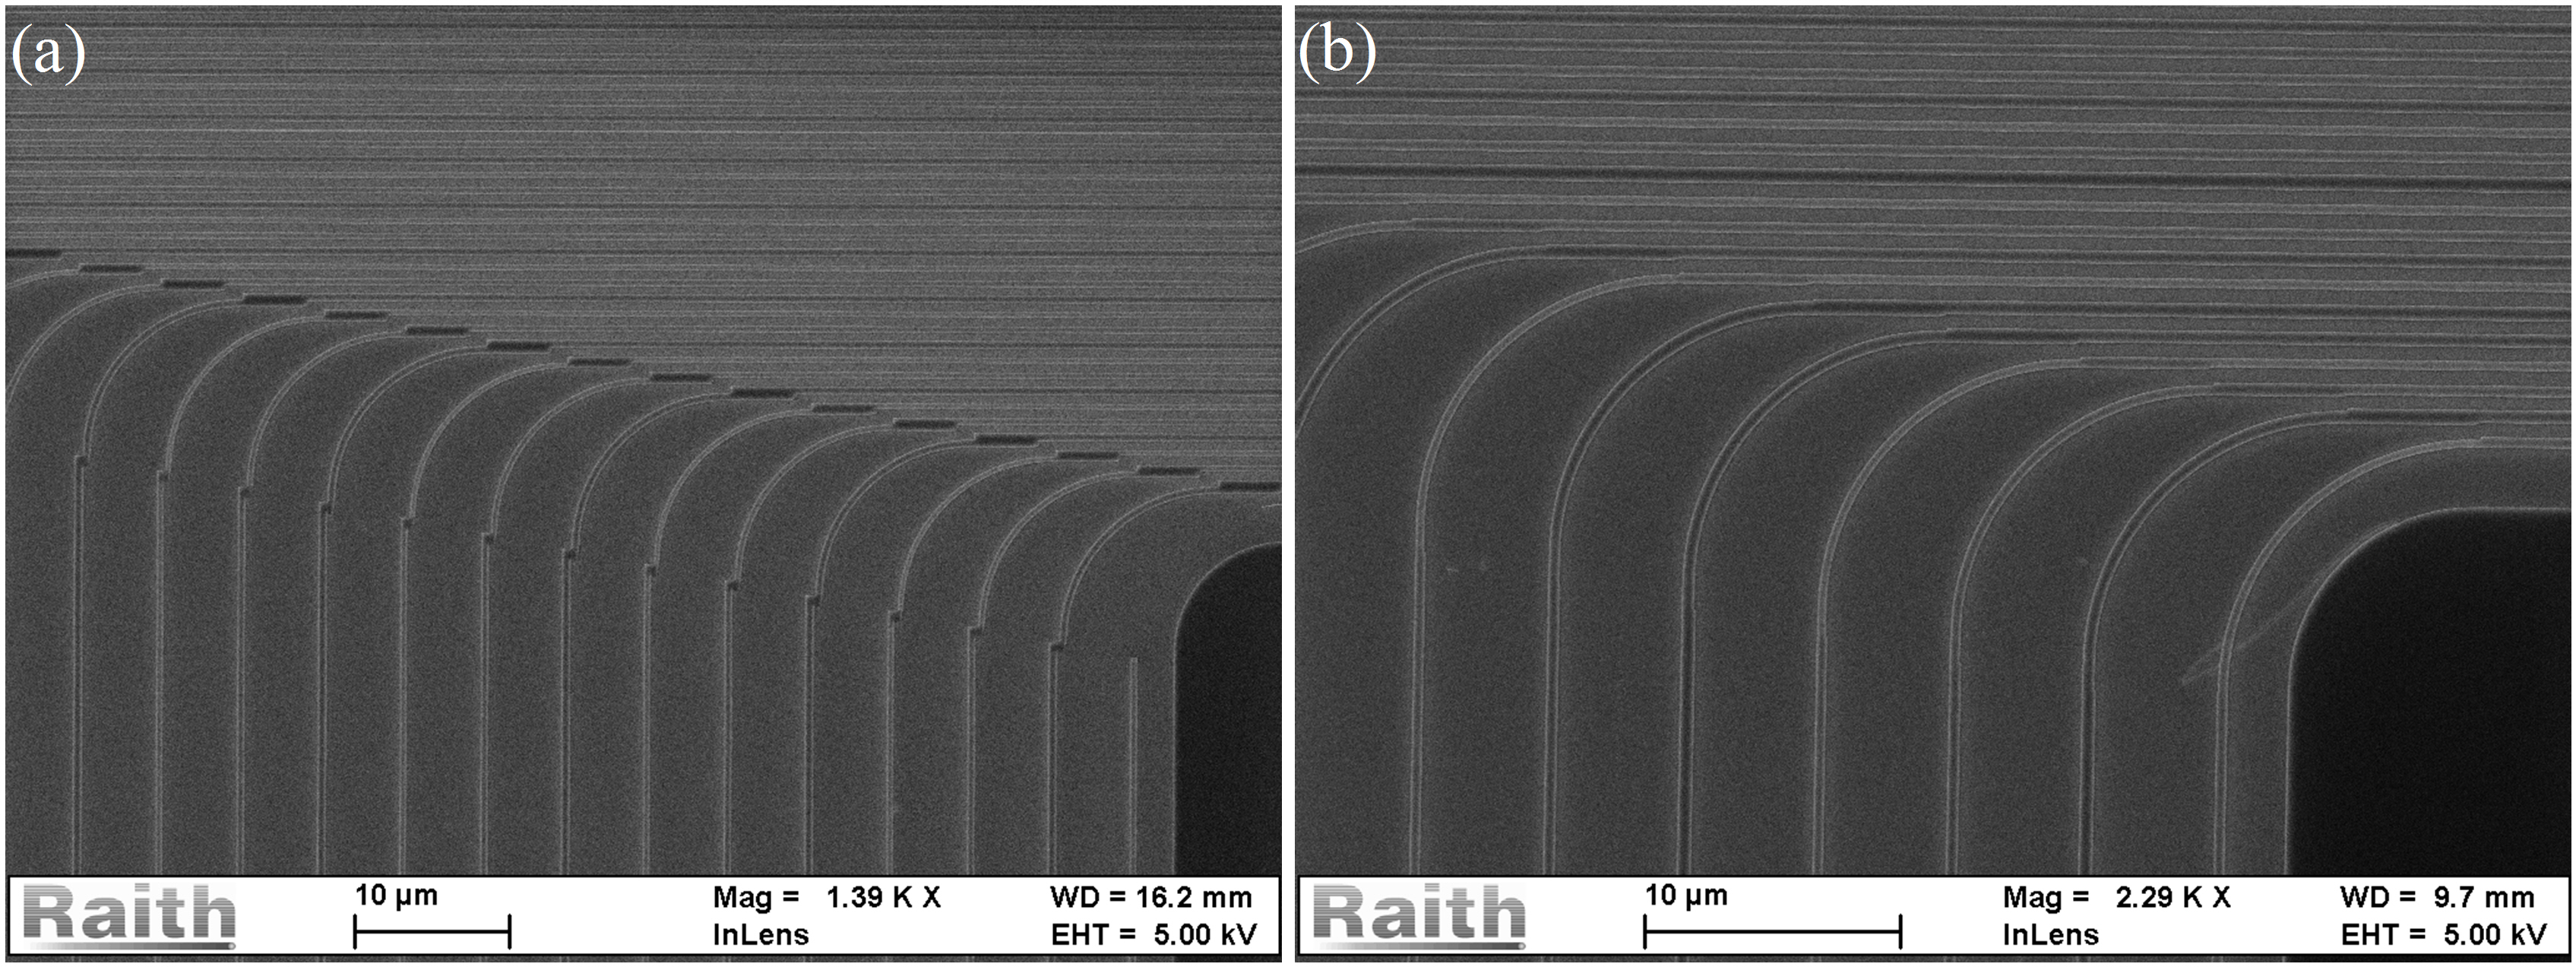
\includegraphics[width=15cm]{./Pictures/edg_misalignment.jpg}
	\captionsetup{justification=centering}
	\caption{EDG光谱仪制作中拼接模式的错位问题,(a)直接用拼接模式制作;(b)经过剂量错位等的补偿}
	\label{edg_misalignment}
\end{figure}

\begin{figure}[htb]
	\centering
	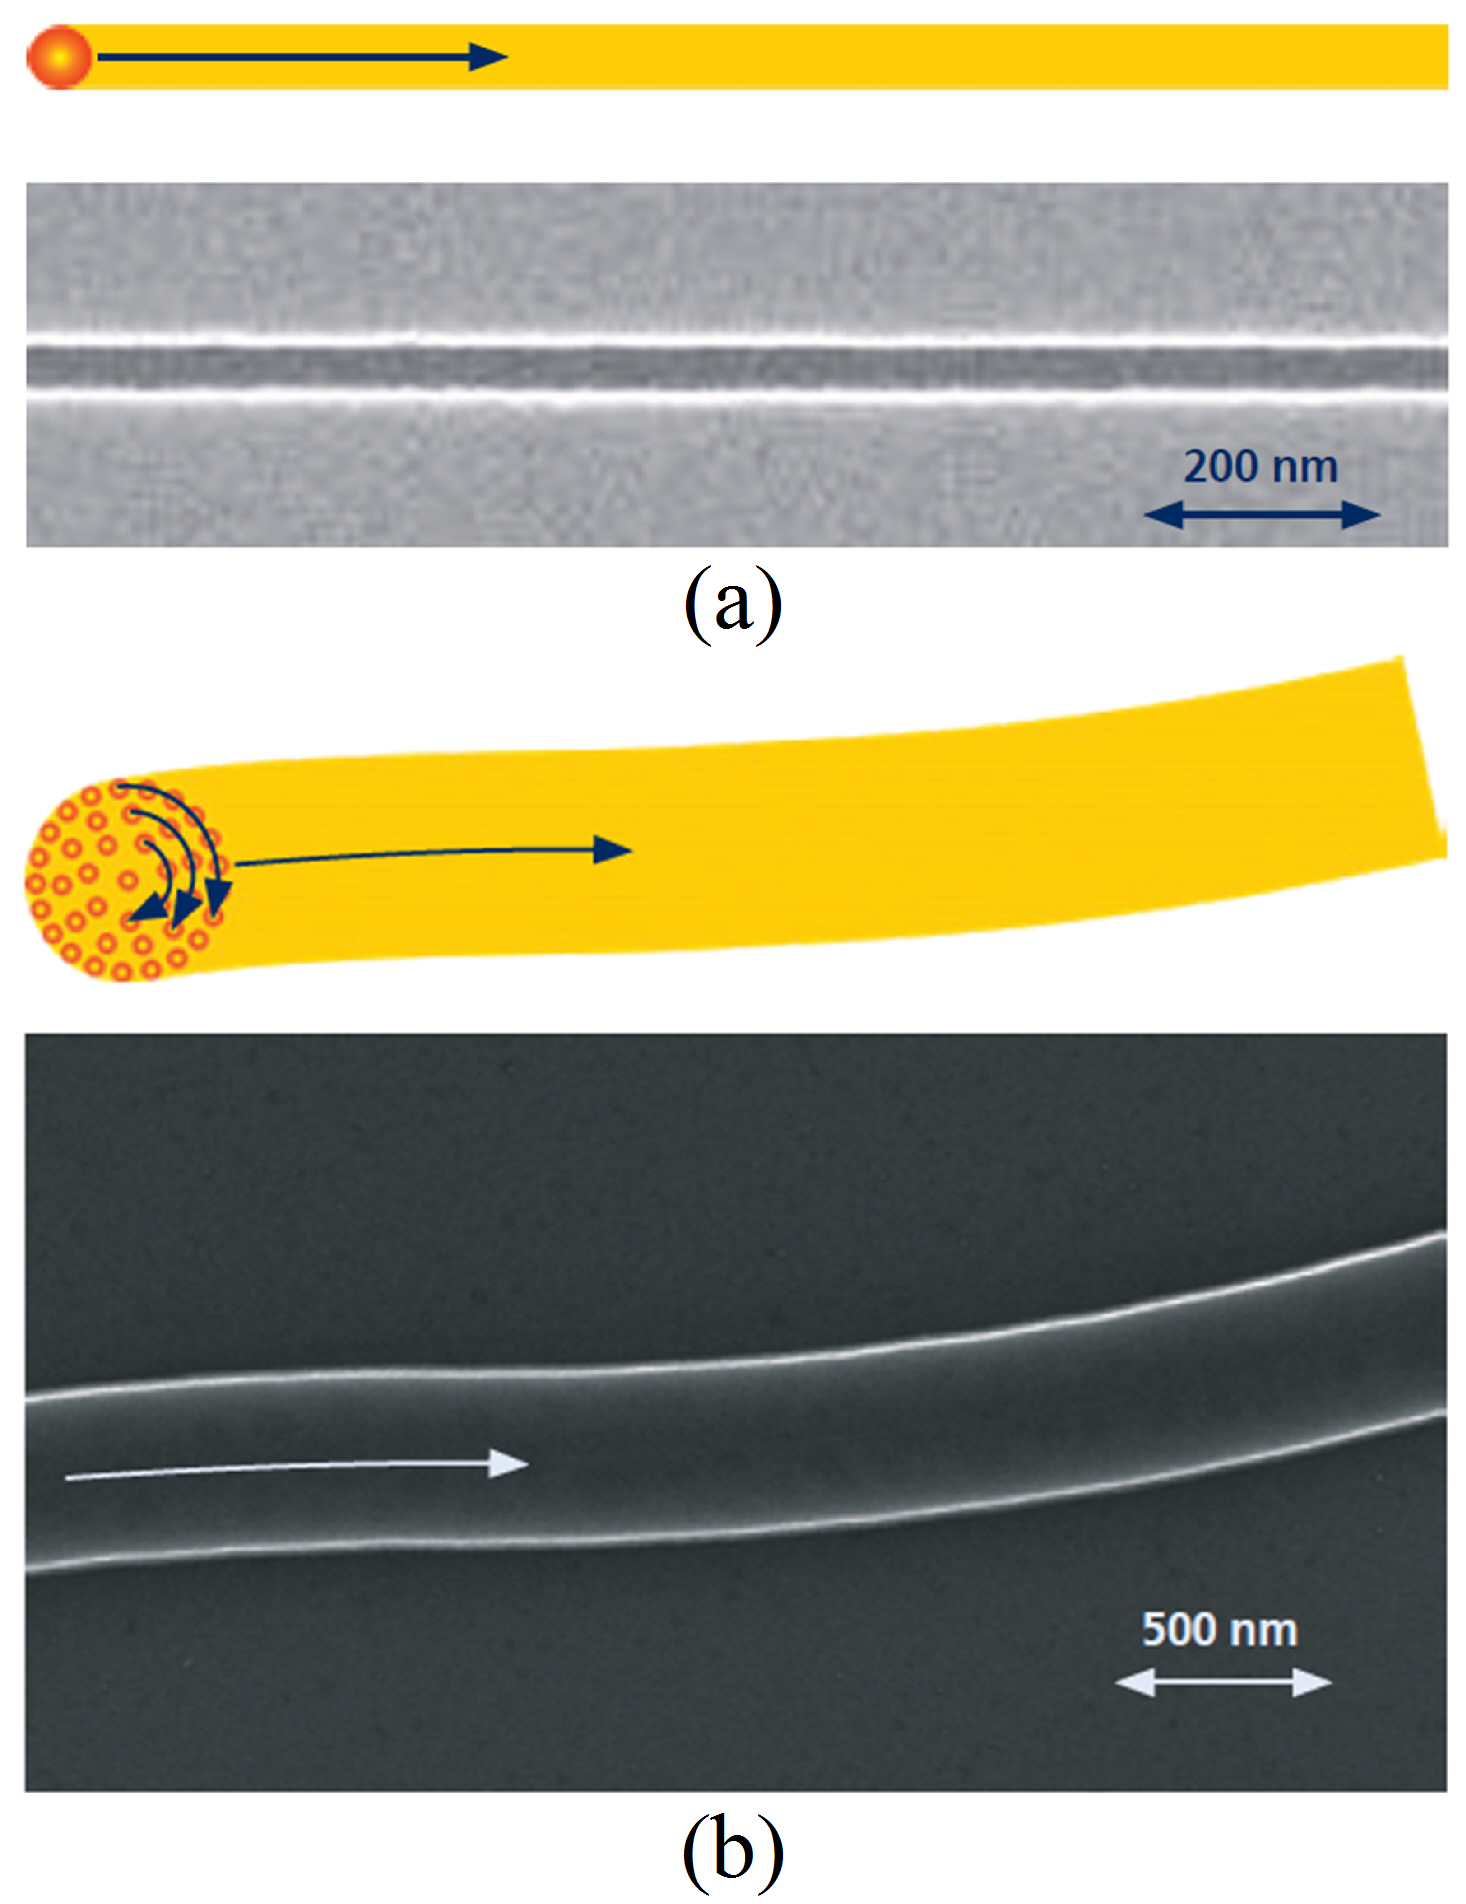
\includegraphics[width=10cm]{./Pictures/edg_fbms.jpg}
	\captionsetup{justification=centering}
	\caption{EBL的两种FBMS模式,(a)高分辨率模式;(b)区域模式}
	\label{edg_fbms}
\end{figure}

连续模式也即FBMS(fixed beam moving stage)模式,如图\ref{edg_pattern_mode}(b)所示,在该模式下,电子枪固定在一个位置,载物台连续移动,相当于进行单点扫描,可以实现零拼接错位。使用该模式可以制作长达数厘米,任意曲线的无错位波导。FBMS模式还可以细分成两种子模式,一种是高分辨率模式,也称为FBMS线条模式,电子束固定在一个点,载物台在水平方向以恒定速率沿设计的方向移动,如图\ref{edg_fbms}(a)所示,图中黄色的点代表固定的电子束。该模式可以用来制作线宽小于20~$nm$的结构。另一种是FBMS区域模式,相较于高分辨模式只能制作线宽较窄的结构,区域模式可以制作宽度达10~$\mu m$的波导。在该模式下,电子束沿不同半径的同心圆高速偏转,同时载物台在横向按设计好的方向以固定速率移动,如图\ref{edg_fbms}(b)所示,图中黄色点代表在做圆周偏转的电子束。因为电子束是按圆对称的方式偏转的,故可以保证载物台在沿不同方向运动的时候都能够得到相同的线宽。

\begin{figure}[htb]
	\centering
	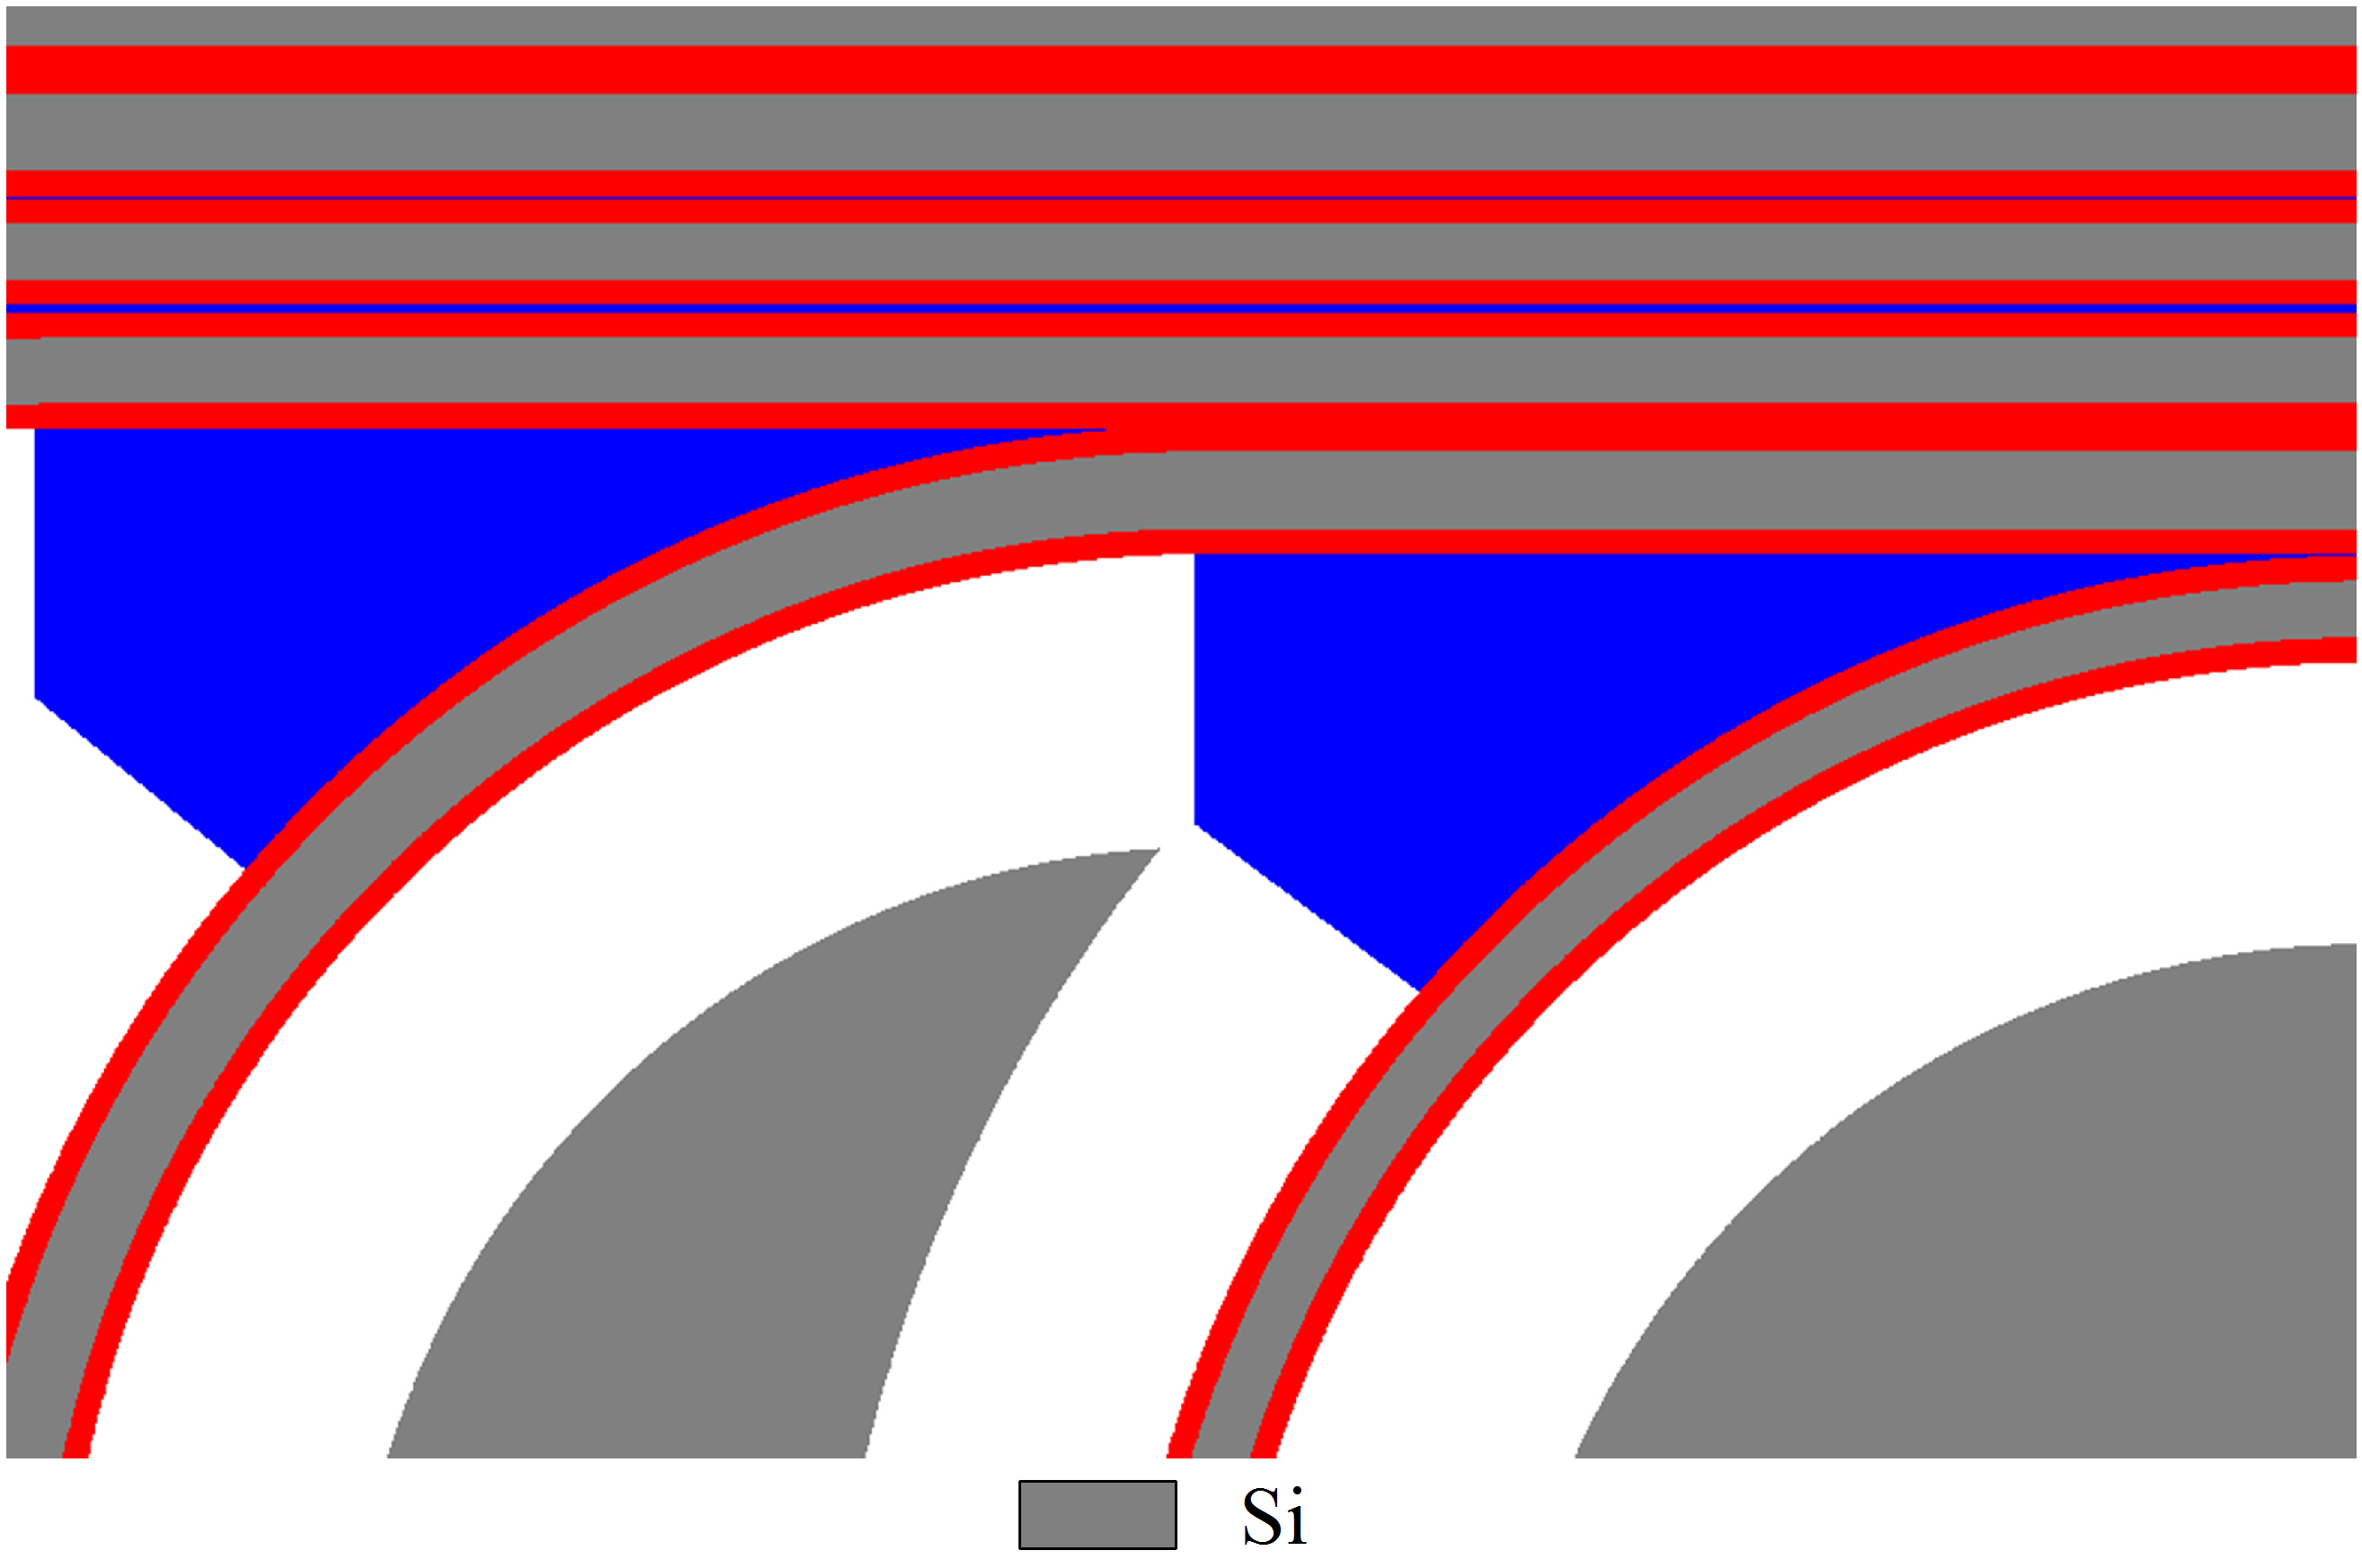
\includegraphics[width=14cm]{./Pictures/edg_miaobian.jpg}
	\captionsetup{justification=centering}
	\caption{EBL描边法制作示意图,灰色之外都是曝光区域}
	\label{edg_miaobian}
\end{figure}

由于我们的EDG光谱仪中含有锥形波导结构,但是FBMS模式只能用来加工宽度不变的波导,而拼接模式对尺寸较大的结构会有拼接错位的问题,所以必须将两种模式结合起来使用。本文采用一种叫做描边法的方法来制作该EDG光谱仪,掩模示意图如图\ref{edg_miaobian}所示,先用FBMS区域模式曝光窄的线条,宽度为200~$nm$,将所有波导的轮廓描绘好,如图\ref{edg_miaobian}中红色线条所示。然后再用拼接模式将一些细小的空隙用多边形填充,如图\ref{edg_miaobian}中的蓝色区域所示。最后我们再用FBMS区域模式曝光较粗的线条,宽度为2.5~$\mu m$,将剩余部分的波导曝光完,如图\ref{edg_miaobian}中的白色区域所示。由于电子束曝光具有临近效应,背向散射电子会到达没有曝光的区域,导致实际曝光的结构会比设计的宽一点,所以,3块图形之间只需要少量的重叠即可,一般取10~$nm$即可,根据实验结果还可以做适当的调整。曝光过程中,一定要首先曝光红色区域,因为红色区域线条较窄,所以总的曝光时间不会太长,对于21通道来说,只需要10~$min$左右,电子枪的位置漂移比较少,故制作的时候可以忽略不计。之后曝光蓝色区域,该区域也只占整个曝光区域一小部分,曝光速度也较快。而且,由于此时红色曝光区域已经定义好了所有波导的边缘,即使蓝色曝光区域发生部分错位也不会影响最后的形成的波导。最后,再曝光2.5~$\mu m$宽的FBMS线条,该曝光过程耗时最长,但此时EDG光谱仪的核心部分,密集阵列波导已经曝光完成,密集阵列波导已经通过90$^{\circ}$弯曲波导分开足够的距离,之后曝光的少许错位对光谱仪的性能影响并不是致命的。

使用FBMS的区域模式曝光200~$nm$窄线条有一个注意事项,在设置EBL的FBMS曝光参数的时候,需要满足公式\ref{fbms_requirement}:

\begin{equation}
\label{fbms_requirement}
\dfrac{Stage~Speed~[mm/s]~*~Defl.~cycle~time~[\mu s]}{Calculation~width~[\mu m]}~<~100
\end{equation}

如果该条件没有被满足,如图\ref{edg_fbms_width}所示,参数Calculation width是加工掩模中FBMS最窄线条的宽度,此处为0.2~$\mu m$,通过该参数,软件内部会计算出Defl. cycle time这个参数为130.0~$\mu s$,Stage Speed由电子枪的电流与曝光剂量等参数共同决定,在使用加速电压30~kV,电子束光阑孔径20~$\mu m$的参数条件下,根据测得的电流大小0.144382~$nA$,我们得到Stage Speed为0.2406367~$mm/s$,代入公式\ref{fbms_requirement}左边我们计算得到156.414,条件不满足。所以曝光过程可能因为载物台移动的速度过快,电子枪在做圆形偏转的时候没有在某处停留足够时间,以达到足够的曝光剂量,本来应该平滑的波导出现波浪形的边缘。我们可以这样来解释波浪形边缘产生的原因,想象有一只笔在纸面上匀速画圆圈,同时将纸沿一个方向匀速移动,如果纸的移动速度过快,我们就会得到一条曲线,但是如果纸移动的速度足够慢,我们就能得到一条均匀的粗直线,粗直线的宽度即为圆圈的直径。如图\ref{edg_ripple}(a)所示,我们可以看到波浪的周期基本固定,说明波浪不是由随机因素影响产生的,我们还可以看到波导弯曲部分相对于直的部分还有些许变窄,这可能是由于曝光过程中的错位引起,这两个因素会导致器件因为损耗太大而没法正常工作。

\begin{figure}[htb]
	\centering
	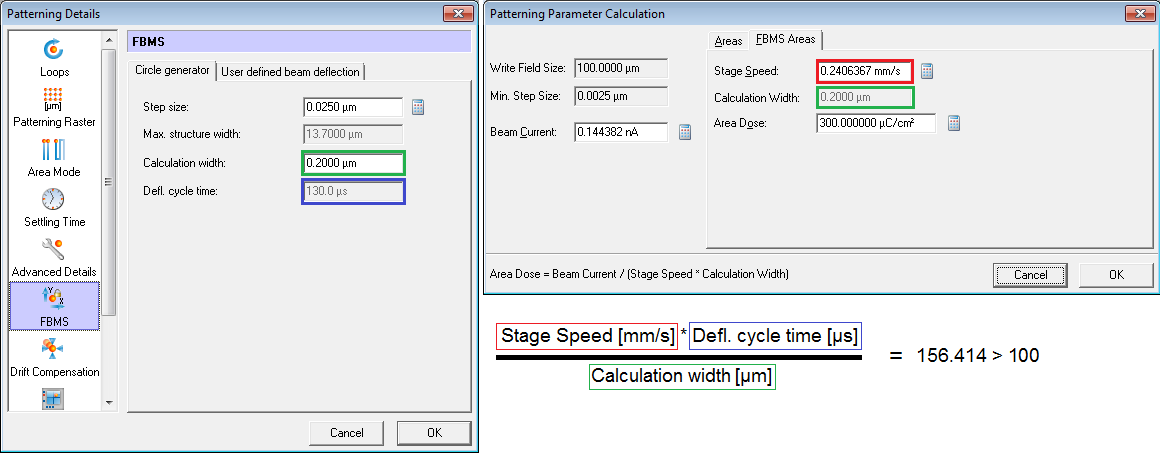
\includegraphics[width=15cm]{./Pictures/edg_fbms_width.png}
	\captionsetup{justification=centering}
	\caption{FBMS曝光模式参数设定}
	\label{edg_fbms_width}
\end{figure}

\begin{figure}[htb]
	\centering
	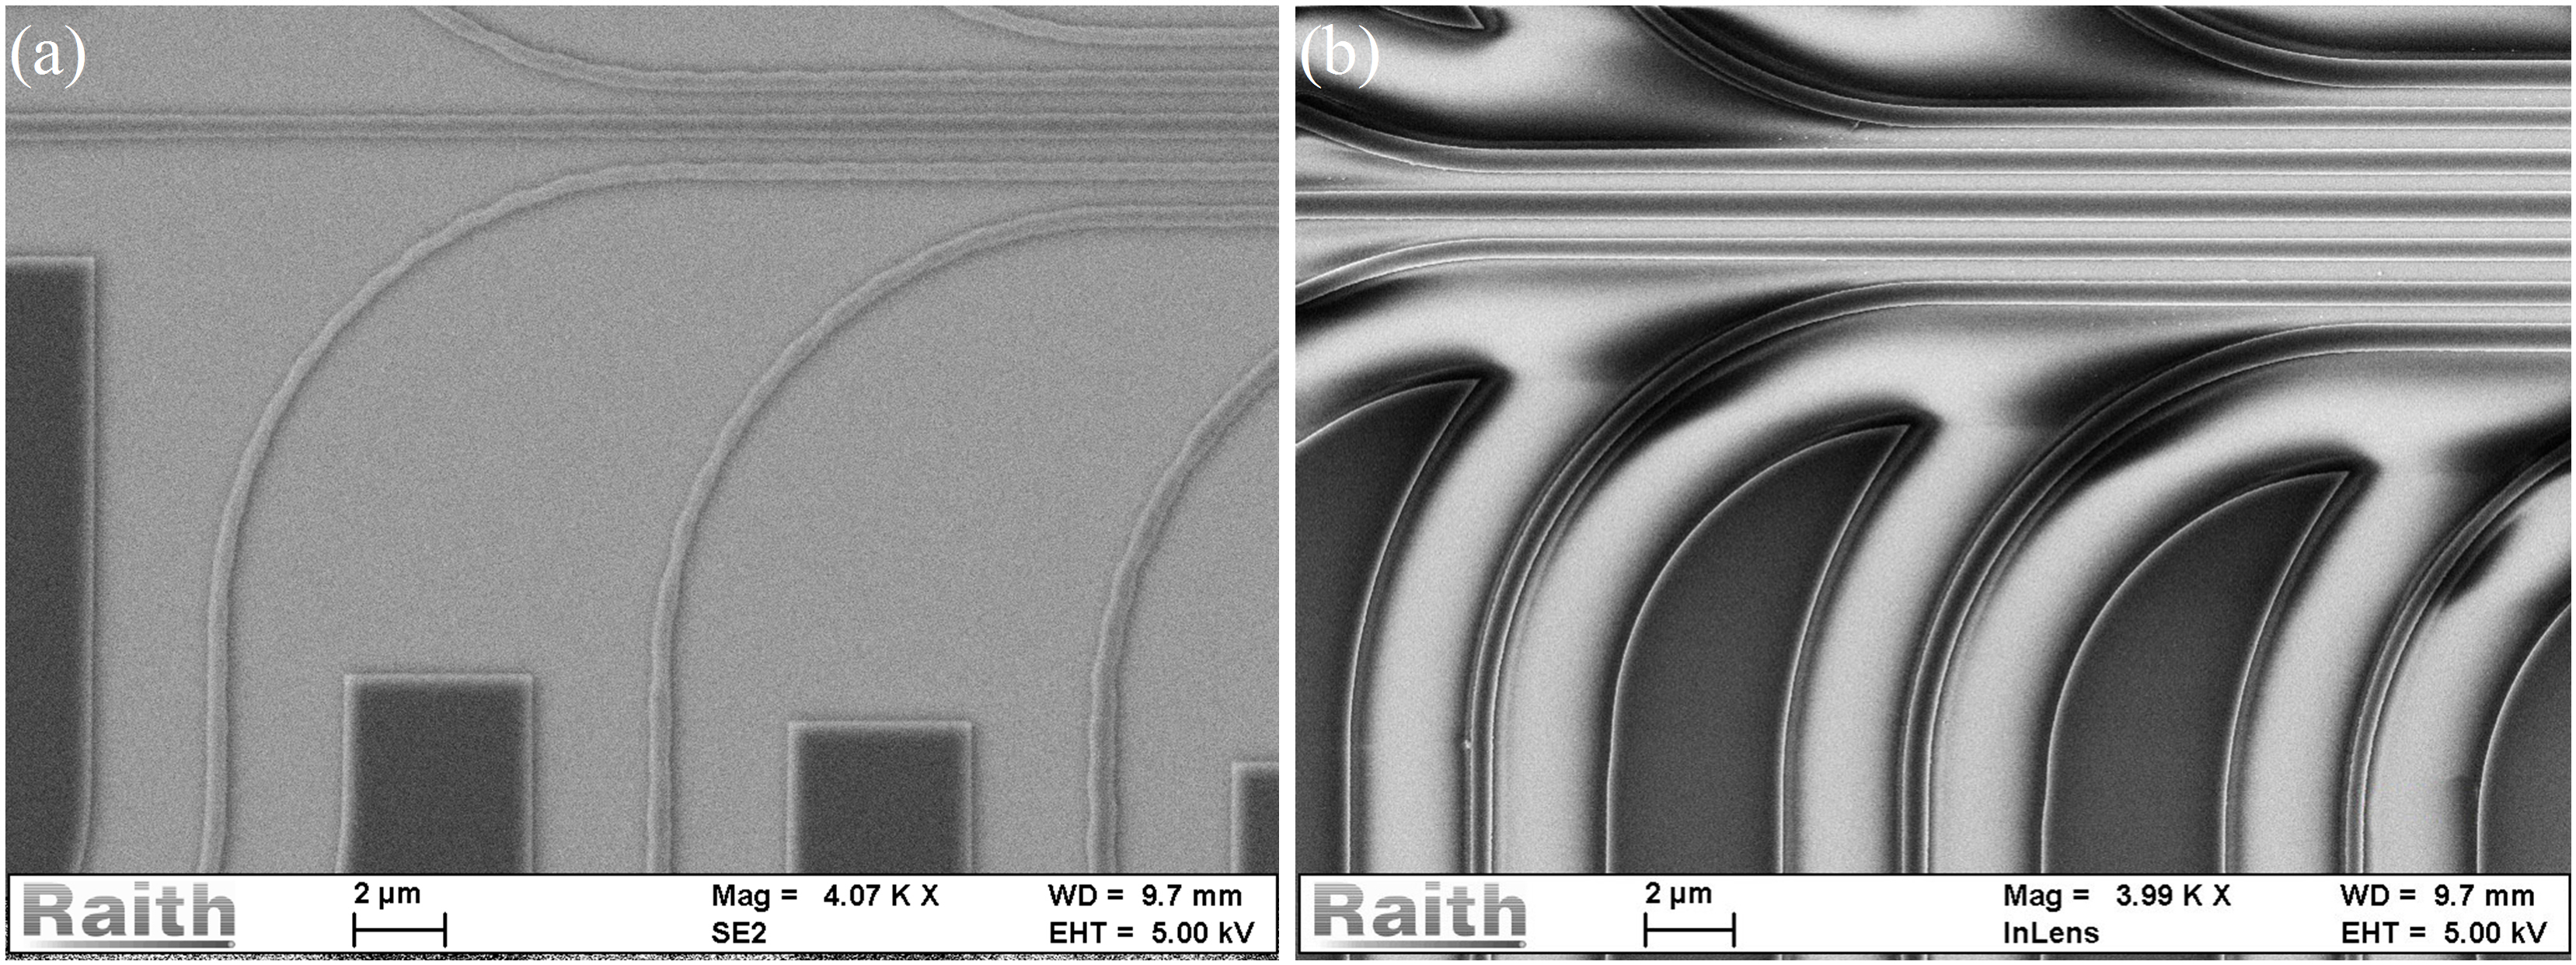
\includegraphics[width=15cm]{./Pictures/edg_ripple.jpg}
	\captionsetup{justification=centering}
	\caption{(a)公式\ref{fbms_requirement}未满足时曝光得到的波导;(b)公式\ref{fbms_requirement}满足后曝光得到的波导}
	\label{edg_ripple}
\end{figure}

为了使公式\ref{fbms_requirement}能够满足,由于Calculation width是我们结构中FBMS模式最小的线宽,无法更改,由其确定的Defl. cycle time参数也就没法修改,故我们只能减慢载物台的移动速度,这可以通过减小EBL电子枪的电流来实现。这就是我们在工艺步骤(c)中,使用的加速电压为20~kV,电子束光阑孔径为10~$\mu m$的原因,此时电子枪的电流可以变成原来的四分之一左右,故Stage Speed也会降低,使得公式\ref{fbms_requirement}得到满足,这也使得我们需要的曝光时间比较长,制作出来的波导结构如图\ref{edg_ripple}(b)所示。从中我们看到制作出来的波导基本光滑,连续模式与FBMS模式之间的错位问题基本消除,可以满足EDG光谱仪的使用要求。

\begin{figure}[htb]
	\centering
	\includegraphics[width=13cm]{./Pictures/edg_fabrication_sem.jpg}
	\captionsetup{justification=centering}
	\caption{硅基EDG光谱仪扫描电镜图,(a)TE浅刻蚀耦合光栅电镜斜视图;(b)波导阵列电镜斜视图;(c)DBR反射光栅电镜俯视图;(d)密集波导阵列电镜俯视图;(e)输入波导电镜俯视图;(f)密集波导阵列细节图}
	\label{edg_fabrication_sem}
\end{figure}

\subsection{制作结果}
我们解理了一块1.5 $cm\times$  1.5~$cm$的SOI芯片,利用EBL描边法制作了该EDG光谱仪,图\ref{edg_fabrication_sem}(a)给出了TE耦合光栅的扫描电镜斜视图,用于将待分析光信号耦合进光谱仪并将分离的光谱耦合出光谱仪;图\ref{edg_fabrication_sem}(b)给出了密集波导阵列的扫描电镜图,可以看到波导在直的与弯曲处都很均匀且光滑;图\ref{edg_fabrication_sem}(c)给出了DBR反射镜的扫描电镜俯视图,我们测得周期为483~$nm$,剩余硅宽度为242~$nm$,跟设计的周期480~$nm$,占空比0.5非常接近,误差主要来源于测量误差。图\ref{edg_fabrication_sem}(d)给出了密集波导阵列的扫描电镜俯视图,测量得到组成密集波导阵列基元的3根波导宽度分别为424~$nm$,488~$nm$和594~$nm$,与设计的420~$nm$,480~$nm$,590~$nm$非常接近,误差主要来自于测量误差。图\ref{edg_fabrication_sem}(e)给出了输入波导的电镜俯视图,从中测得输入波导末端的宽度为798~$nm$,与设计的800~$nm$的误差主要来自测量误差。图\ref{edg_fabrication_sem}(f)给出了密集波导阵列的细节图,从中我们可以看到不同宽度的波导都渐变到同一个宽度,这可以改善该EDG光谱仪的通道均匀性。

\section{硅基EDG光谱仪的测试}
\subsection{无源垂直耦合测试系统}

\begin{figure}[htb]
	\centering
	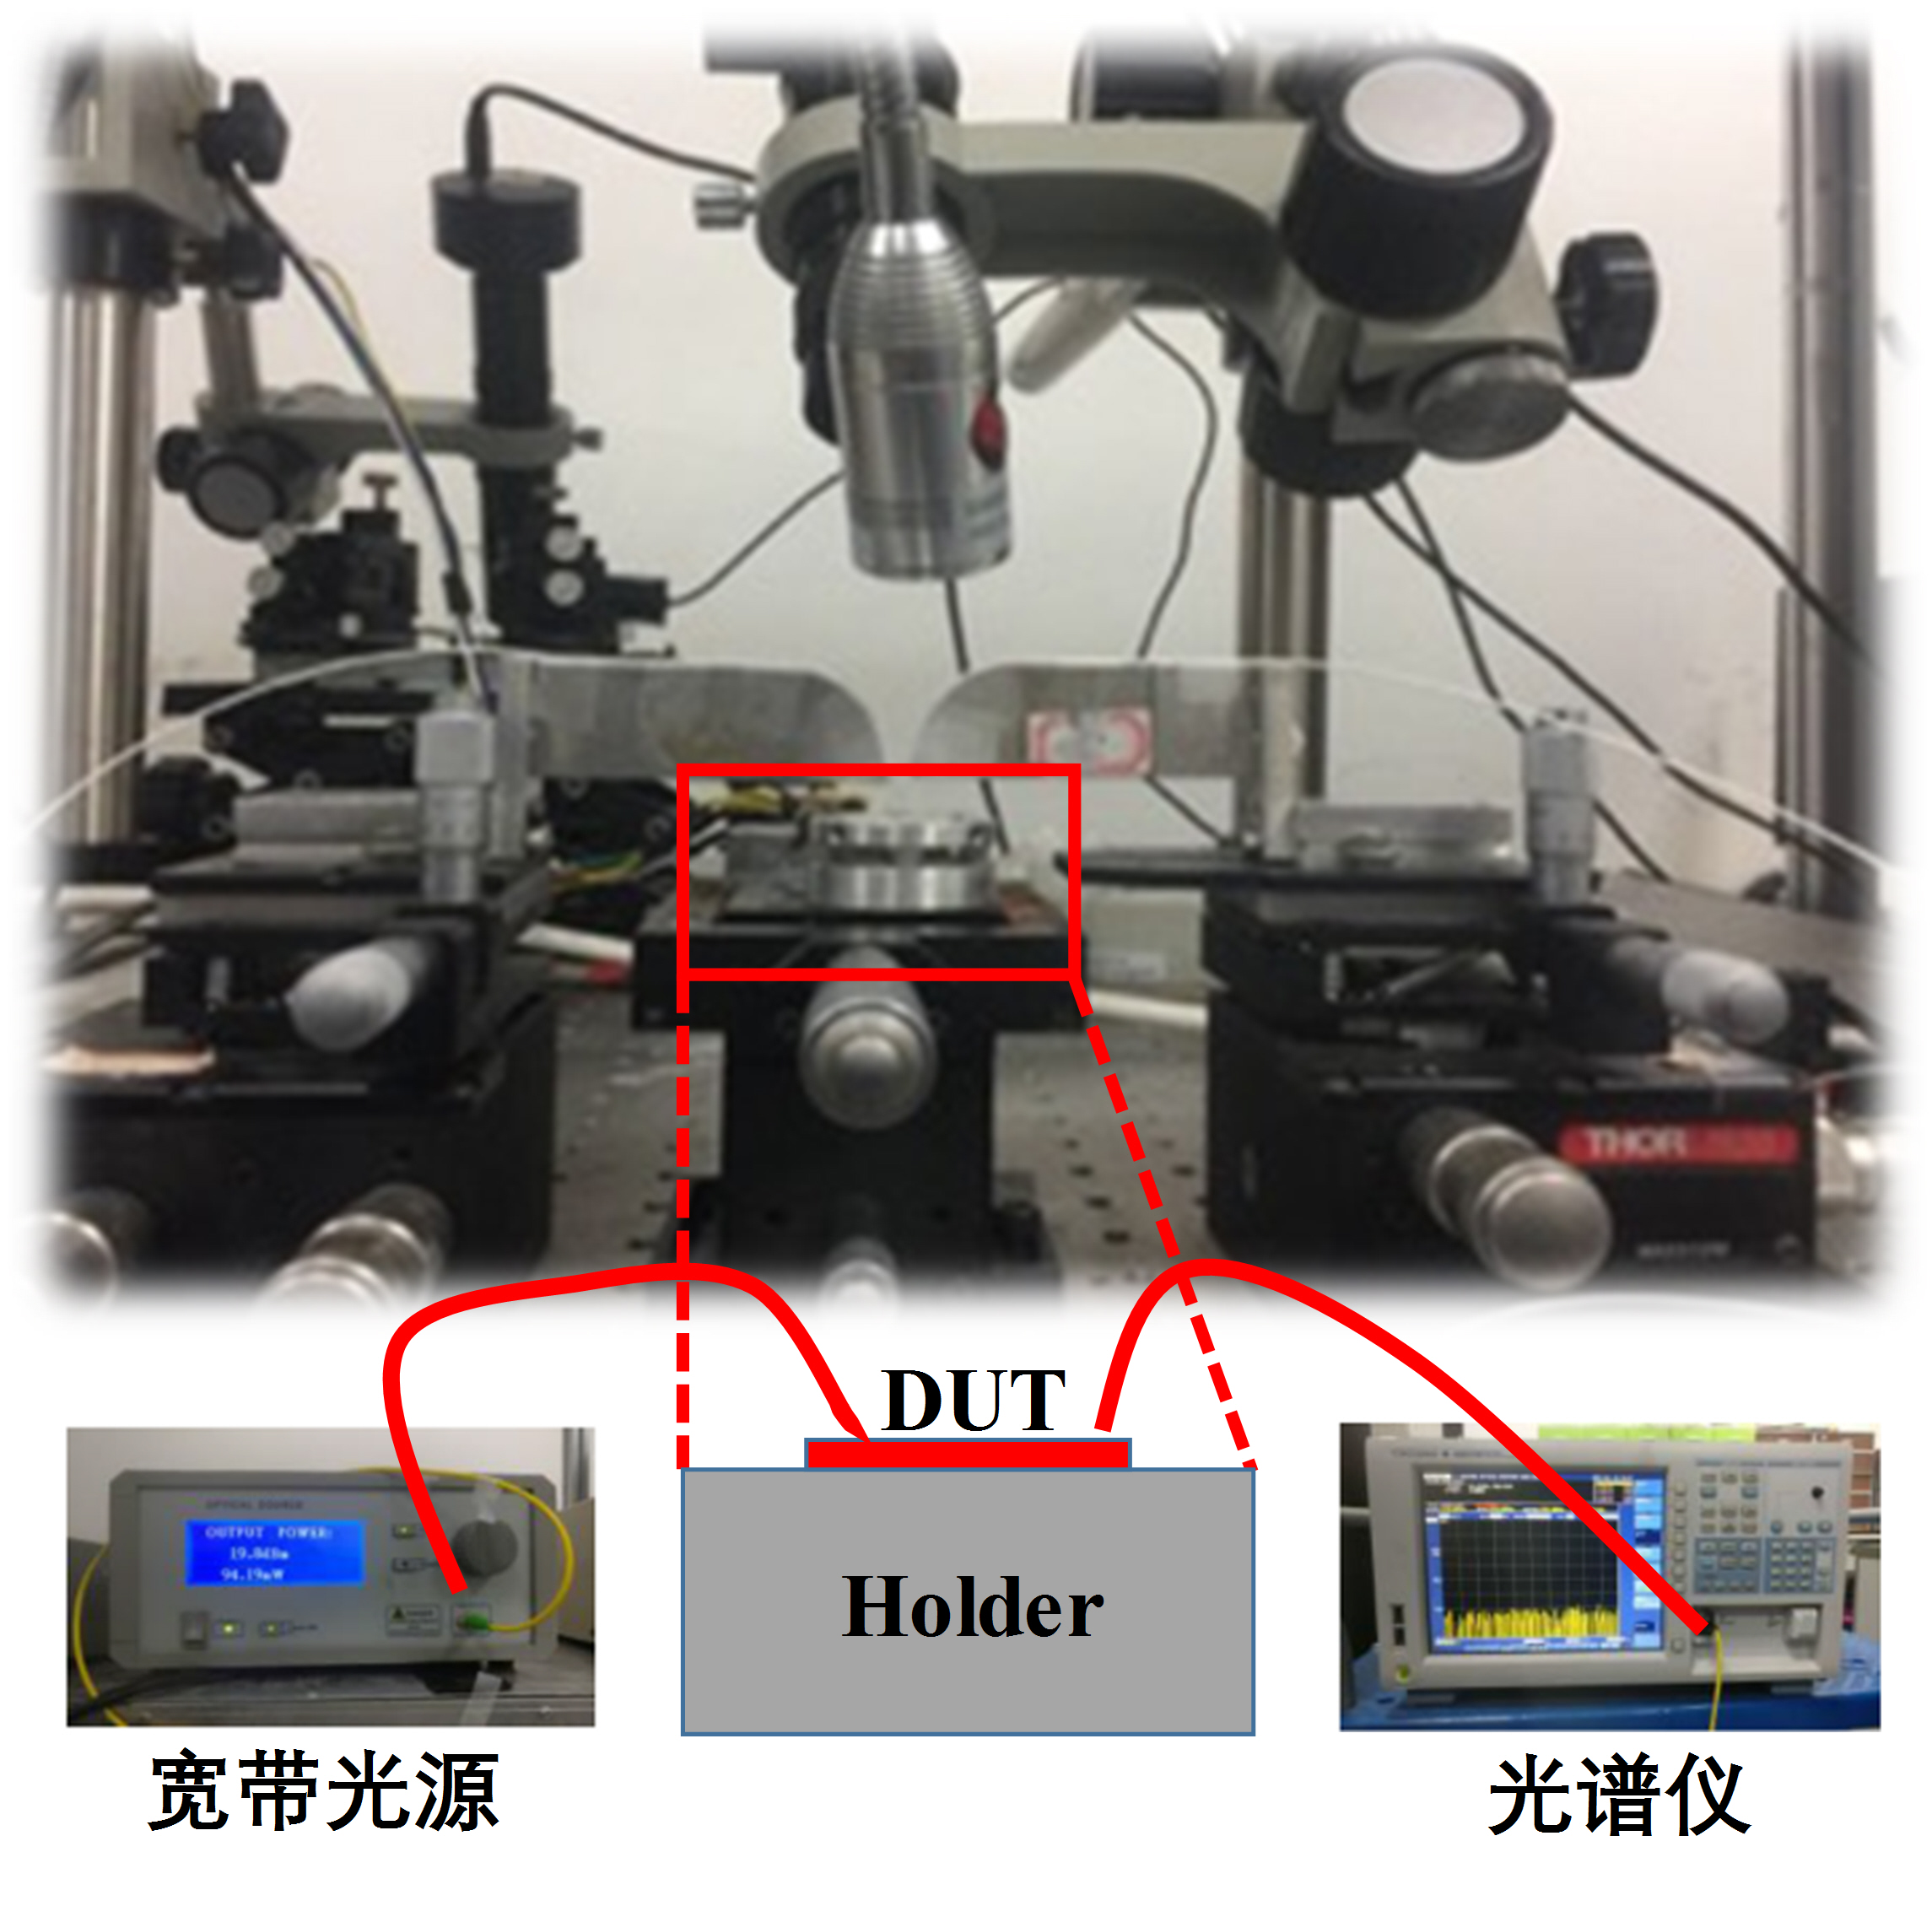
\includegraphics[width=12cm]{./Pictures/edg_setup.jpg}
	\captionsetup{justification=centering}
	\caption{垂直耦合系统,DUT:device under test}
	\label{edg_setup}
\end{figure}

测试光芯片通常有两种耦合方式,一种是端面耦合,其优点是可以减少硅基工艺步骤,工作带宽大,偏振不敏感及易于封装等优点。但对于具有高折射率差的SOI平台,其波导尺寸横截面尺寸在亚微米量级,其模式与光纤的模式失配严重,故想要获得较高的耦合效率,就需要引入较长的模式转换结构来减小波导与光纤之间的模式失配程度,因此也会使得器件的长度边长。而且,端面耦合时为了获得较高的耦合效率,往往还需要对端面进行抛光处理。这些因素使得端面耦合丧失了本身能带来的优势,同时也增加了工艺的复杂度。另一种是垂直耦合,其利用在波导末端刻蚀衍射光栅的方式,使得波导中的光场衍射到芯片上表面被光纤所接收,从而实现耦合。该耦合方式虽然存在封装麻烦,带宽有限而未能在商业化器件中得到大规模应用,但是其可以在片子的任意位置实现光场的输入输出耦合,故其在器件测试阶段提供了极大的便利。本文即是采用垂直耦合系统来进行EDG光谱仪的测试表征,该垂直耦合系统如图\ref{edg_setup}所示。该系统固定于气浮光学减震平台上,待测芯片放于一个可以二维调节的载物平台上。载物平台上方是照明光源与显微镜系统,用来进行光纤与耦合光栅的对准。载物平台两边是两个六维调节架,每个调节架上都固装有可以用来固定并调整光纤耦合角度的刀臂。如前文所述,我们在EDG光谱仪制作过程中已经集成了TE浅刻蚀耦合光栅,其参数为:周期640~$nm$,占空比0.5,刻蚀深度70~$nm$,耦合角度15$^{\circ}$。该光栅耦合损耗为\~{}4~dB,中心波长\~{}1550~$nm$,3~dB带宽\~{}60~$nm$。在EDG光谱仪测试过程中光栅的响应曲线通过直波导已经归一化。

本文测试使用的光源为放大自发辐射(amplified spontaneous emission, ASE)宽带光源(B\&A technology OS814),该光源可以提供在1550~$nm$附近80~$nm$带宽的光谱,由1550~$nm$波段单模光纤传输到芯片的耦合光栅,光场经过芯片后,从耦合光栅输出再次耦合进另一根单模光纤并导入商用高分辨率光谱仪(Yokoyawa AQ6370D),光谱仪的分辨率设为0.2~$nm$。

\begin{figure}[htb]
	\centering
	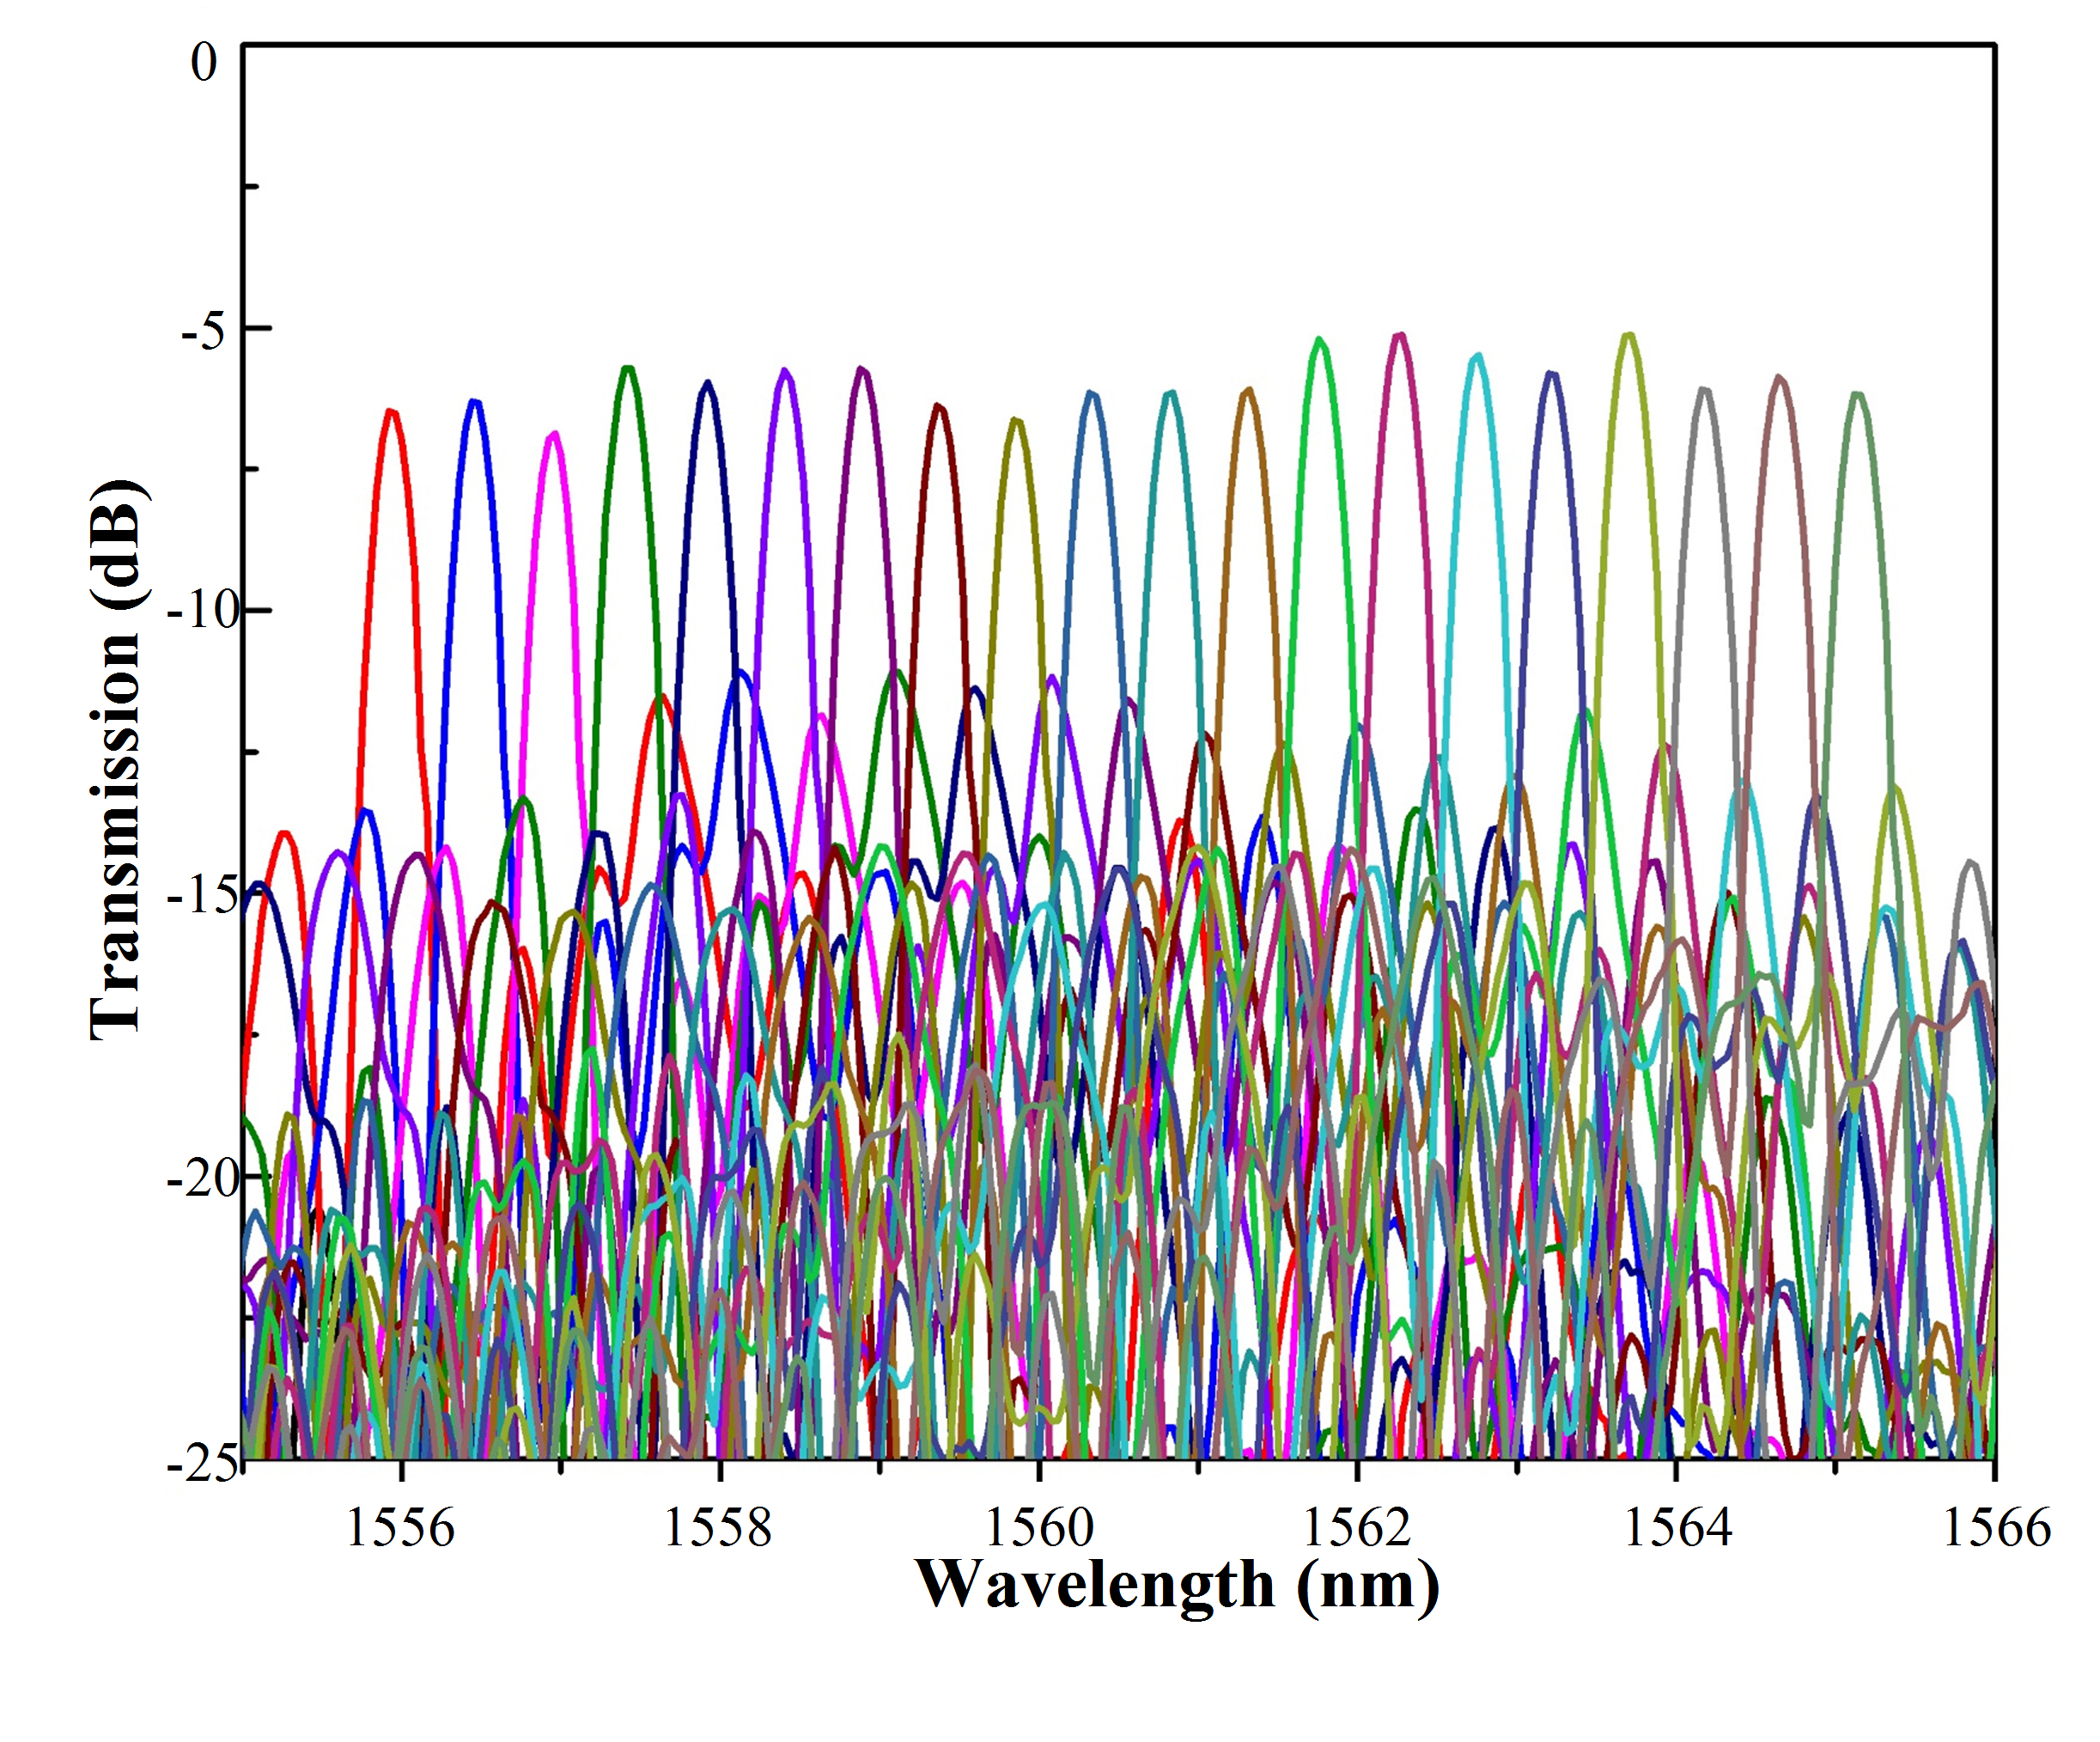
\includegraphics[width=12cm]{./Pictures/edg_transmission.jpg}
	\captionsetup{justification=centering}
	\caption{EDG光谱仪的传输谱线}
	\label{edg_transmission}
\end{figure}

\subsection{硅基EDG光谱仪的测试结果}

使用上述测试平台,我们得到EDG光谱仪的传输谱线如图\ref{edg_transmission}所示。我们只测到了20个通道,其中一个边缘通道因为工艺问题损耗过大没有在图中给出。从图中我们看到光谱仪的分辨率为0.5~$nm$,与设计值一致,通道的3~dB带宽为
0.28~$nm$,对应的光谱分辨率($\lambda/\Delta\lambda$)为5571,最大插入损耗为6.9~dB,最大串扰为-4.3~dB。一般EDG的串扰主要是由自由传输区的不均一造成的相位差,但是从图\ref{edg_transmission}中可以看到通道中周期性的旁瓣是该EDG光谱仪串扰的主要来源。造成这些旁瓣的原因是,我们采用拼接模式曝光的反射光栅部分,而且该部分尺寸非常大,故会有拼接错位问题,导致原本的反射镜中叠加了这一种周期性的错位,从而使得EDG光谱仪的测试谱线中出现旁瓣\cite{he1998monolithic,xie2018silicon}。该EDG光谱仪的损耗主要有以下几个来源,首先是我们因为加工时间的考虑,DBR反射镜我们只采用了3个周期,使得其反射率不是很高,考虑其刻蚀过程中产生的垂直度与侧壁粗糙,损耗有2~dB,再者是光栅在曝光过程中的漂移,使得其成像的质量下降,类似于产生了离焦的效果,使得部分能量不能耦合进入输出波导,还有波导侧壁粗糙引起的散射损耗。成像质量的下降不仅会使得器件的损耗变大,而且也会增加器件的串扰,因为一部分没有耦合进相应输出波导的光能量会耦合进入旁边通道。同样,波导的粗糙侧壁也使得波导中的光能量通过辐射耦合进相邻波导,从而增加了光谱仪的串扰\cite{melati2014optical}。该EDG光谱仪的通道不均匀性为1.7~dB,主要由两个原因引起。一,由于曝光时间过长引起的通道不均匀性,后面曝光的波导会有更多的错位问题,我们可以看到中间波导的通道均匀性明显比边缘的要好。二,不同宽度的波导损耗不同,较窄的波导往往会比较宽的波导有更大的损耗,因为其有更多的模场与因ICP刻蚀造成的粗糙侧壁相互作用。根据Vlasov等人测试得到的结果,在220~$nm$~SOI平台上,400~$nm$,450~$nm$,500~$nm$的波导的损耗分别为33.8~dB/$cm$,7.4~dB/$cm$,2.4~dB/$cm$\cite{vlasov2004losses},我们的波导长度平均在350~$\mu m$左右,采用这边最大的损耗与最低的损耗进行粗略估算,损耗差约为1~dB,故我们可以得知不同宽度的波导造成了部分通道不均匀性。如果能采用半导体公司流片的方式制作该EDG光谱仪,损耗与串扰的性能将得到很大的提升。

我们比较了该EDG光谱仪与其他人最近制作的EDG光谱仪,结果如列表\ref{spectrometer_comparison}所示,虽然我们制作的EDG光谱仪在损耗与串扰方面的性能没有其他几个好,但是其在分辨率上显示出了最好的性能而且有潜力在9 $mm^{2}$的范围内实现121个通道,这在其他几种设计中都没法实现。

\begin{table}[htb]
	\zihao{5}
	\captionsetup{justification=centering}
	\caption{基于EDG的光谱仪性能比较,中心波长均为1550~$nm$}
	\label{spectrometer_comparison}
	\centering
	\begin{tabular}[t]{|c|c|c|c|c|}
		\hline
		\textbf{Reference} & This work & Pommarede\cite{pommarede201716} & Xie\cite{xie2018silicon} & Ryckeboer\cite{ryckeboer2013silicon} \\
		\hline
		\textbf{Platform} & 220~$nm$~SOI & 300~$nm$~SOI & 300~$nm$~SiN & 220~$nm$~SOI\\
		\hline
		\textbf{Insertion loss (dB)} & 6.9 & 1.8 & 1.39 & 5\\
		\hline
		\textbf{Non-uniformity (dB)} & 1.7 & 0.5 & 1.2 & \~{}1\\
		\hline
		\textbf{Crosstalk (dB)} & -4.3 & -15 & -30 & -16\\
		\hline
		\textbf{Channel spacing (nm)} & 0.5 & 0.8 & 5 & 3.2\\
		\hline
		\textbf{Resolution ($\pmb{\lambda/\Delta\lambda}$)} & \textbf{{\color{red}5571}} & 4822 & 1300 & Not given \\
		\hline
		\textbf{Number of channels} & 20 & 16 & 5 & 8 \\
		\hline
		\textbf{Footprint ($\pmb{mm^{2}}$)} & 9 & 2.6 & 3 & 0.56\\
		\hline
	\end{tabular}
\end{table}

\section{本章小结}
本章首先介绍了气体检测的基本原理,并根据本文所制作的自脉冲DFB激光器与基于EDG的高分辨率光谱仪设计了一套气体浓度检测系统。本章对实现片上光谱仪的一些方案做了背景介绍,分析了各种实现方案的优缺点。随后对其中基于EDG的方案设计并优化了121通道的光谱仪,分别从输出波导阵列和反射光栅两个方面进行了优化。波导阵列方面我们采用了模式复用中经常用到的密集阵列波导,第一次将其应用到EDG中,将本来SOI平台上间距2.5 $\mu m$,5 $\mu m$的波导间距缩小到只有1 $\mu m$,密集阵列波导的串扰控制在-40 dB以下,大大增加了基于EDG的光谱分辨率。在反射光栅方面,我们采用DBR反射镜,对其位置用两个完美成像点的方法进行了优化,并通过扫描绝对光程,提升了边缘通道的性能。之后根据该设计进行了超净室的工艺制作,受限于仪器的加工能力,只制作了20通道的EDG光谱仪。在实验过程中,采用了一种称为EBL描边法的加工工艺来改善加工过程中的错位问题。最后测得该EDG光谱仪的通道间隔为0.5~$nm$,通道的3~dB带宽为0.28~$nm$,光谱分辨率($\lambda/\Delta\lambda$)为5571,插入损耗约为6.9~dB,最大串扰为-4.3~dB,通道不均匀性为1.7~dB。测试的结果并不理想,本章详细地对其进行了解释,如果采用光刻流片的方式进行加工,DBR反射镜与阵列波导的错位问题将得到改善,器件的性能将得到很大的提升。
